\documentclass[10pt, openany]{book}
\usepackage[FINAL]{../boilerplate/rexx} 
\usepackage{hyperref}
\usepackage{graphics}
\usepackage{fontspec}
% \fontspec
%      [ Path = /Users/rvjansen/Fonts/,
%        BoldFont       = MinionPro-Bold.otf ,
%        ItalicFont     = MinionPro-It.otf ,
%        BoldItalicFont = MinionPro-BoldIt.otf ]
%      {MinionPro-Regular.otf}
% \fontspec
%      [ Path = /Users/rvjansen/Fonts/,
%        BoldFont       = SourceCodePro-Bold.otf ]
%      {SoureCodePro-Regular.otf}

\setmainfont[Mapping=tex-text]{Minion Pro}
\setmonofont[Mapping=tex-text,Scale=0.80]{Source Code Pro}
\usepackage{tabularx}
\usepackage{booktabs}
\usepackage{makeidx}
\usepackage[all]{xy}
%\usepackage{lingmacros}
\usepackage{color}
\usepackage{xcolor}
\usepackage{listings}
\usepackage{caption}
\usepackage{longtable}
\usepackage{colortbl}
\usepackage{framed}
\usepackage{fancyvrb}
\definecolor{shadecolor}{rgb}{0.9,0.9,0.9}
\usepackage{alltt}
\DeclareCaptionFont{white}{\color{white}}
\DeclareCaptionFormat{listing}{\colorbox{gray}{\parbox{\textwidth}{#1#2#3}}}
\captionsetup[lstlisting]{format=listing,labelfont=white,textfont=white}
\usepackage{listings}
\usepackage[official]{eurosym}
\makeatletter
\lst@CCPutMacro\lst@ProcessOther {"2D}{\lst@ttfamily{-{}}{-{}}}
\@empty\z@\@empty
\makeatother
\lstdefinelanguage{NetRexx}
{morekeywords={abstract,adapter,binary,case,catch,class,constant,dependent,deprecated,digits,do,else,end,engineering,extends,final,finally,for,forever,if,implements,indirect,import,indirect,inheritable,interface,iterate,label,leave,loop,method,native,nop,numeric,options,otherwise,over,package,parent,parse,private,properties,protect,public,return,returns,rexx,say,scientific,set,digits,form,select,shared,signal,signals,sourceline,static,super,then,this,until,used,upper,volatile,when,where,while},
sensitive=false,
extendedchars=false,
morecomment=[s]={/*}{*/},
morecomment=[l]{--},
morecomment=[s]{/**}{*/},
morestring=[b]",
morestring=[d]",
morestring=[b]',
morestring=[d]'}

\lstset{language=NetRexx,
  captionpos=t,
  tabsize=3,
  alsolanguage=Rexx,
  keywordstyle=\color{blue},
  commentstyle=\color{cyan},
  stringstyle=\color{red},
  numbers=left,
  numberstyle=\tiny,
  numbersep=5pt,
  breaklines=true,
  showstringspaces=false,
  index=[1][keywords],
  columns=flexible,
  basicstyle=\fontsize{8}{8}\fontspec{Source Code Pro},emph={label}}

\usepackage{../boilerplate/rail}
\usepackage{pst-barcode,pstricks-add}
\usepackage{bashful}
\usepackage{metalogo}
\usepackage{marginnote}
\usepackage{pdfpages}
\usepackage{float}
\hyphenation{Net-Rexx Net-Rexx-A Net-Rexx-C Net-Rexx-R Mac-OSX
  infra-structure im-ple-men-ta-tion-de-pen-dent}
\makeindex
\DeclareGraphicsExtensions{.jpg,.png}
\setlength{\parskip}{4pt}
\setlength{\parindent}{0pt}
\usepackage{enumitem}
\newcommand{\nr}{Net\textsc{Rexx}}
\newcommand{\Rexx}{R\textsc{exx}}
\newcommand{\nrpackagename}{\splice{java GetPackageName}}
\newcommand{\minimalJVMversion}{1.6}
\newcommand{\keyword}[1]{\texttt{#1}}
\newcommand{\code}[1]{\texttt{#1}}
\newcommand{\thisyear}{\splice{java TexYear}}
\newcommand{\ecjjarname}{ecj-4.6.3.jar}
\newcommand{\msd}[1]{\msdhelper#1\relax}
\newcommand{\msdhelper}[1]
  {\ifx\relax#1\else
    \ifx-#1--{}\else#1\fi
    \expandafter\msdhelper\fi}
  \newcommand{\doublehyphen}{\mbox{\msd{``-~-''}}}
  \newcommand{\doublehyphenunquoted}{\mbox{\msd{-~-}}}
%%% Local Variables: 
%%% mode: latex
%%% TeX-master: t
%%% End: 

\begin{document}
\renewcommand{\isbn}{978-90-819090-3-7}    
\setcounter{tocdepth}{1} 
\title{\fontspec{Bodoni URW Light}Pipelines for \nr{} QuickStart Guide}
\author{Ed Tomlinson \and Jeff Hennick \and René Jansen}
\date{Version \splice{java org.netrexx.process.NrVersion} of \today}
\maketitle
\pagenumbering{Roman}
\pagestyle{plain}
\frontmatter
\pagenumbering{Roman}
\pagestyle{plain}
\section*{Publication Data}
\textcopyright  Copyright The Rexx Language Association, 2011-\splice{java TexYear}
%\\

All original material in this publication is published under the Creative Commons - Share Alike 3.0 License as stated at \url{http://creativecommons.org/licenses/by-nc-sa/3.0/us/legalcode}.\\[0.5cm]
The responsible publisher of this edition is identified as \emph{IBizz IT Services and Consultancy}, Amsteldijk 14, 1074 HR Amsterdam, a registered company governed by the laws of the Kingdom of The Netherlands.\\[1cm]
This edition is registered under ISBN \isbn \\[1cm]
\psset{unit=1in}
\begin{pspicture}(3.5,1in)
  \psbarcode{\isbn}{includetext guardwhitespace}{isbn}
\end{pspicture}
\newpage
%%% Local Variables:
%%% mode: latex
%%% TeX-master: t
%%% End:

\tableofcontents
\newpage
\pagenumbering{arabic}
\frontmatter
\large
\chapter*{\fontspec{IBM Plex Serif}\LARGE The \nr{} Programming Series}
This book is part of a library, the \emph{\nr{} Programming Series}, documenting the \nr{} programming language and its use and applications. This section lists the other publications in this series, and their roles. These books can be ordered in convenient hardcopy and electronic formats from the Rexx Language Association.
\newline
\newline
\begin{tabularx}{\textwidth}{>{\bfseries}lX}
\toprule
%% Quick Start Guide & This guide is meant for an audience that has done some programming and wants to start quickly. It starts with a quick tour of the language, and a section on installing the \nr{} translator and how to run it. It also contains help for troubleshooting if anything in the installation does not work as designed, and states current limits and restrictions of the open source reference implementation.
%% \\\midrule
Programming Guide & The Programming Guide is the one manual that at the same time teaches programming, shows lots of examples as they occur in the real world, and explains about the internals of the translator and how to interface with it.
\\\midrule
Language Reference & Referred to as the NRL, this is meant as the formal definition for the language, documenting its syntax and semantics, and prescribing minimal functionality for language implementers.
\\\midrule
Pipelines Guide \& Reference & The Data Flow oriented companion to \nr{}, with its CMS Pipelines compatible syntax, is documented in this manual. It discusses running Pipes for \nr{} in the command shell and the Workspace, and has ample examples of defining your own stages in \nr{}.
\\\bottomrule
\end{tabularx}
%%% Local Variables: 
%%% mode: latex
%%% TeX-master: t
%%% End: 

\chapter{Typographical conventions}
In general, the following conventions have  been observed in the NetRexx publications:
\begin{itemize}
\item Body text is in this font
\item Examples of language statements are in a \textbf{bold} type
\item Variables or strings as mentioned in source code, or things that appear on the console, are in a \texttt{typewriter} type
\item Items that are introduced, or emphasized, are in an \emph{italic} type
\item Included program fragments are listed in this fashion:
\begin{lstlisting}[label=example,caption=Example Listing]
-- salute the reader
say 'lectorem salutat'
\end{lstlisting}
\item Syntax diagrams take the form of so-called \emph{Railroad Diagrams} to convey structure, mandatory and optional items
\begin{rail}
AggregateExpression : ("AVG" |"MAX" |"MIN" |"SUM")
 (
   (
    'DISTINCT' ?  StateFieldPathExpression
   ) | 'COUNT'
   (
    'DISTINCT' ?  IdentificationVariable
                  | StateFieldPathExpression
                  | SingleValuedAssociationPathExpression
   )
 )
   ;
\end{rail}
%%% Local Variables: 
%%% mode: latex
%%% TeX-master: t
%%% End: 
\end{itemize}
\mainmatter
\chapter{Introduction}
A Pipeline, or Hartmann
Pipeline\footnote{\url{//https://en.wikipedia.org/wiki/CMS_Pipelines}}\footnote{This
  page used to be called Hartmann Pipeline, but was renamed to CMS Pipelines
  in 2016}, is a concept that extends and improves pipes as they are known from Unix and other operating systems. The name pipe indicates an interprocess communication mechanism, as well as the programming paradigm it has introduced. Compared to Unix pipes, Hartmann Pipelines offer multiple input- and output streams, more complex pipe topologies, and a lot more.

Pipelines were first implemented on VM/CMS, one of IBM's mainframe
operating systems. This version was later adapted to run under
MUSIC/SP and TSO/MVS (now z/OS) and has been part of several product configurations. Pipelines are
widely used by VM users, in a symbiotic relationship with REXX, the
interpreted language that also has its origins on this platform.

Pipes for \nr{} is the implementation of Pipelines for the Java Virtual
machine. It is written in \nr{} and pipes and stages can be defined using this
language. It can run on every platform that has a JVM
(Java Virtual Machine) installed. This portable version of Pipelines was started
by Ed Tomlinson in 1997 under the name of \emph{njPipes}, when \nr{} was
still very new, and was open sourced in 2011, soon after the \nr{}
translator itself. The included stages have always been open source. It was integrated into the \nr{} translator in
2014 and first released with version 3.04.

In version 3.08, there are
important improvements that enable pipelines to be run from the
command line, and from the \nr{} REPL program \emph{nrws}, the
\nr{} Workspace. The pipes compiler has been renamed
\emph{pipc}, while the pipes runner component keeps using the name \emph{pipe}.

\chapter{The Pipeline Concept}
\section{What is a Pipeline?}
The \emph{pipeline} terminology is a set of metaphores derived from
plumbing. Fitting two or more pipe segments together yields a
pipeline. Water flows in one direction through the pipeline.

There is a source, which could be a well or a water tower; water is
pumped through the pipe into the first segment, then through the other
segments until it reaches a tap, and most of it will end up in the
sink. A pipeline can be increased in length with more segments of
pipe, and this illustrates the modular concept of the pipeline.

When we discuss pipelines in relation to computing we have the same
basic structure, but instead of water that passes through the
pipeline, data is passed through a series of programs (\emph{stages})
that act as filters.

Data must come from some place and go to some place. Analogous to the
well or the water tower there are \emph{device drivers} that act as a
source of the data, where the tap or the \emph{sink} represents the place the
data is going to, for example to some output device as your terminal
window or a file on disk, or a network destination.

Just as water, data in a pipeline flows in one direction, by
convention from the left to the right.
\section{Stage}
A program that runs in a pipeline is called a \emph{stage}. A program
can run in more than one place in a pipeline - these occurrences
function independent of each other. 

The pipeline specification is processed by the \emph{pipeline
  compiler}, and it must be contained in a character string; on the
commandline, it needs to be between quotes, while when contained in a
file, it needs to be between the delimiters of a \nr{} string. An
solid vertical bar | is used as \emph{stage separator}, while other characters
can be used as an option when specifiying the
local option for the pipe, after the pipe name.\footnote{In versions
  before Pipelines for \nr{} 3.08, the default was the exclamation
  mark (!), which use was discontinued in favour of conformity with
  VM/CMS Pipelines.}

When looking a two adjacent segments in a pipeline, we call the left
stage the \emph{producer} and the stage on the right the
\emph{consumer}, with the \emph{stage separator} as the connector.
\section{Device Driver}
A \emph{device driver} reads from a device (for instance a file, the
command prompt, a machine console or a network connection) or writes
to a device; in some cases it can both read and write. An example of a
device drivers are \texttt{<} and \texttt{>} ; these read and write data from and to files.

A pipeline can take data from one input device and write it to a
different device. Within the pipeline, data can be modified in almost
any way imaginable by the programmer.

The simplest process for the pipeline is to read data from the input
side and copy it unmodified to the output side. Chapter
\ref{ch:devicedrivers} on page \pageref{ch:devicedrivers} shows the
currently supported input- and output devices. The pipeline compiler
connects these programs; it uses one program for each device and
connects them together.

The inherent characteristic of the pipeline is that any program can be
connected to any other program because each obtains data and sends
data throug a device independent standard interface. This becomes
apparent when data can be in-line (specified or generated within the
pipeline specification), come in (or be output) to devices like disk
or tape, or be handled through a network -- all these formats can be
processed by the same stages.

The pipeline usually processes one record (or line) at a time. The
pipeline reads a record for the input, processes it and sends it to
the output. It continues until the input source is drained.

\chapter{Running pipelines}
There are a number of ways to specify and run a pipeline. A little
setup is necessary.

\section{Configuration}
The required configuration is minimal. The \nr{}F.jar (java archive
file) needs to be on the classpath environment variable (\nr{}C.jar, which is smaller, will suffice when there is a working javac compiler). Also, the current directory (.) needs to be on the classpath.
It is convenient to have aliases or shell scripts defined as abbreviations for the invocation of the pipe, pipc (pipe compiler) and nrc (netrexx compiler) utility programs. 
Aliases are preferable because some shell processors have
idiosyncrasies in the treatment of script arguments. With an alias we
can be sure that every \nr{} program sees its arguments the same
way.
\begin{verbatim}
.bash_aliases:
alias pipc="java org.netrexx.njpipes.pipes.compiler"
alias pipe="java org.netrexx.njpipes.pipes.runner"
alias nrc="java org.netrexx.process.\nr{}C"
\end{verbatim}
For Windows, the following works: file \texttt{pipe.bat}:
\begin{verbatim}
@java -cp "%NETREXX_HOME%\lib\NetRexxF.jar;%CLASSPATH%" org.netrexx.njpipes.pipes.runner %*
\end{verbatim}
For Windows, the following works: file \texttt{pipc.bat}:
\begin{verbatim}
@java -cp "%NETREXX_HOME%\lib\NetRexxF.jar;%CLASSPATH%" org.netrexx.njpipes.pipes.compiler %*
\end{verbatim}

\begin{shaded}
Do note that the Windows .bat files assume that the NETREXX\_HOME
environment variable is set correctly, that is, to the top of the path
where NetRexx is installed. This prepends the NetRexxF.jar file to an
already existing CLASSPATH. For the development of local classes (that is, all precompiled pipelines), a
dot ('.'), needs to be on this CLASSPATH.
\end{shaded}
These aliases (or command scripts (in Windows it is called a batch
file) enable you to do the following:

To run a pipeline from the commandline, type:
\begin{lstlisting}
pipe 'gen 100 | dup 999 | count words | console'
\end{lstlisting}

Remember to use double quotes on Windows shells. When the \texttt{pipe}
alias or command script is not on your path, you can also use:

\begin{lstlisting}
java org.netrexx.njpipes.pipes.runner 'gen 100 | dup 999 | count words | console'
\end{lstlisting}

In both cases the answer should be 100000 - you have generated one
hundred thousand lines, but fortunately you did not print them, but
only counted them. To see them all, you can insert a | console | stage
in between the dup and the count stage.

After we have verified the working of the command processors, we will
discuss in the next section which possibilities you have for running
pipelines in day-to-day usage.



\section{From the \nr{} Workspace (nrws) with direct execution}
The first way is the most straightforward, and highly recognizable for
users of CMS Pipelines, as it mimics the way a pipe is run in the CMS
3270 interface. It also yields the best response time, specially when
the \texttt{nrws.input} file in your home directory preloads the Pipes subsystem, as in this
example:
\begin{verbatim}
-- preload the pipe machinery for good response on first pipe
pipe literal Pipelines processor loaded. | console
\end{verbatim}
This is not magic: we do a Pipe execution (that displays: ``Pipe
processor loaded'') which loads all necessary classes and leaves them
in memory. We can then type this command after the \emph{nrws>}
prompt.
\begin{figure}[h]
  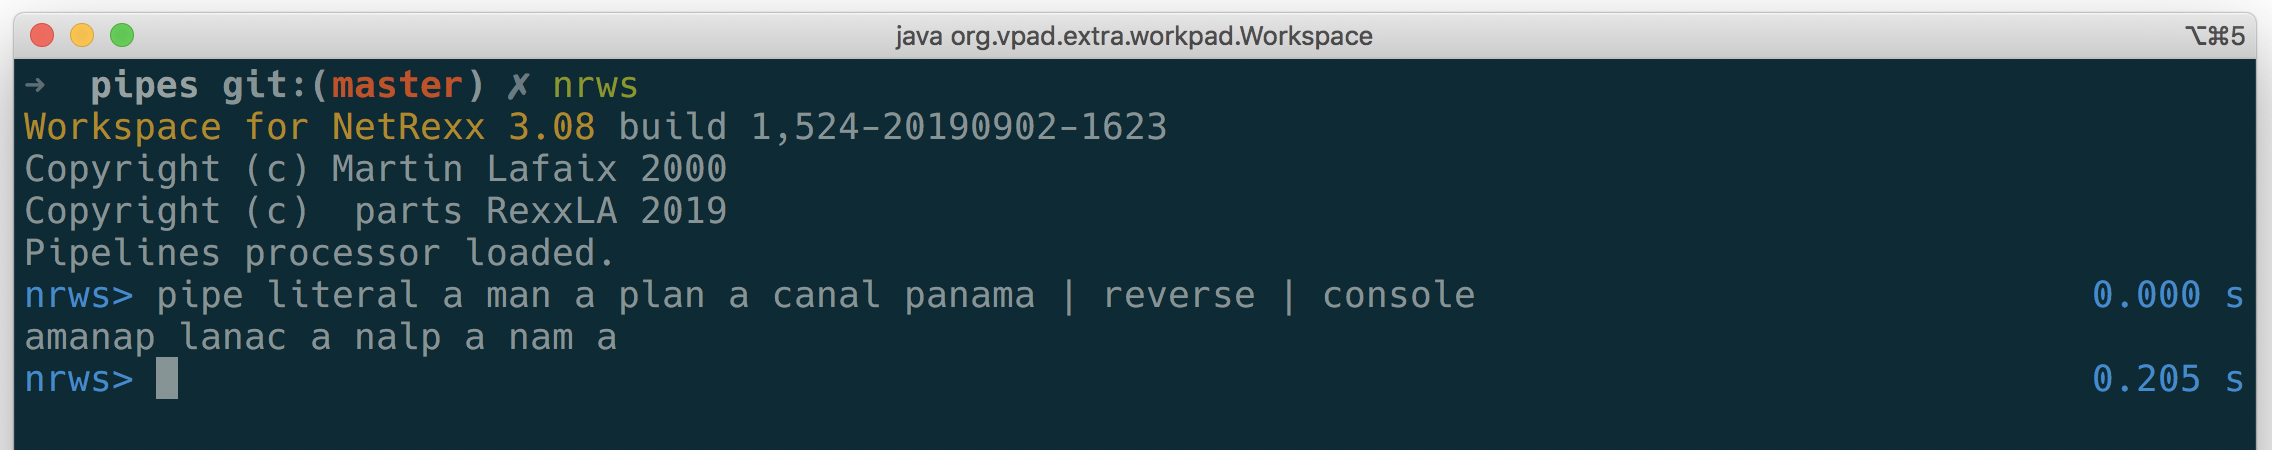
\includegraphics[width=0.75\textwidth]{images/runnrws.png}
  \caption{Run in the \nr{} Workspace}
  \label{fig:runnrws}
\end{figure}

\begin{lstlisting}
pipe literal a man a plan a canal panama | reverse | console
\end{lstlisting}
Executed this way, the executed class image will not be written to
disk. The \emph{timing} option is great for prototyping and
performance work.
\section{From the command line with direct execution}
The only difference is that after the \texttt{pipe} command,
the rest of the specification needs to be quoted in the command shells
of Linux, Windows and macOS. In CMS, the pipeline specification can
also be quoted - in this way, a pipeline can be entirely
portable. Windows needs double quotes, zVM/CMS does not need quotes,
but if they are used they need to be double quotes. macOS and Linux
can use single or double quotes, in most cases.
\begin{lstlisting}
pipe "literal a man a plan a canal panama | reverse | console"
\end{lstlisting}
\begin{figure}[h]
  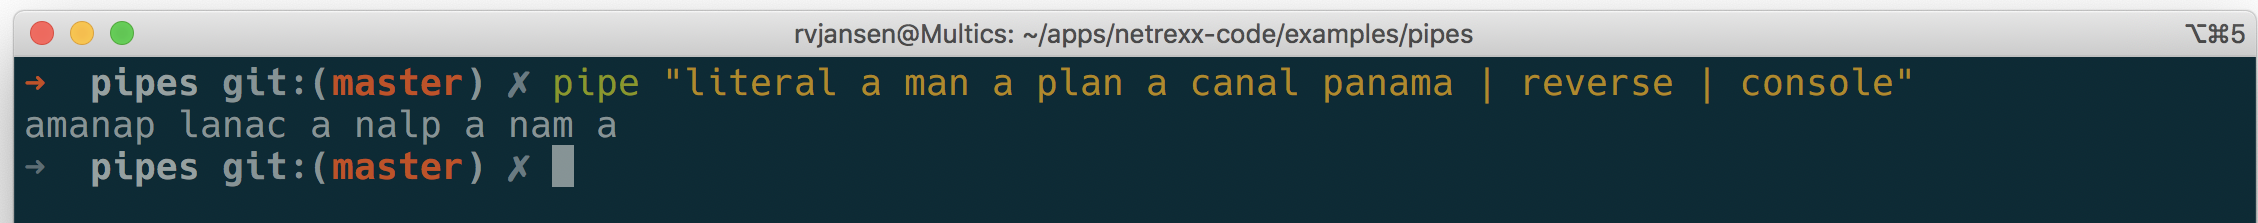
\includegraphics[width=0.75\textwidth]{images/runfromshell.png}
  \caption{Run from the OS command line}
  \label{fig:runfromshell}
\end{figure}

Executed this way, the executed class image again will not be written to
disk.

% When the pipe is named, for example test1 with a (test1) prologue, this name will be used for the class image, instead of a generated unique name. Naming a pipe will enable specification of options for the compiler, like the pipe separator character.
% \begin{lstlisting}
% pipe "(test1 sep !) literal a man a plan a canal panama ! reverse !
% console"
% \end{lstlisting}
% As of pipes for \nr{} 3.08 the default separator is the | (pipe)
% symbol, as in zVM/CMS. The above example shows how to use the previous
% default, the exclamation mark.
\section{Precompiled Pipelines}
In this mode, which uses the \texttt{pipc} command (for pipe
compiler), a .class file will be persisted to disk. This class can be
run as many times as needed, without the overhead of compilation. This
also would be the right mode for pipes that take different arguments when re-run.
The pipe name needs to be specified, and will be the class name. When
the class name exists, it will be overwritten.
\begin{lstlisting}
pipc "(test1) literal a man a plan a canal panama | reverse | console"
\end{lstlisting}
\begin{figure}[h]
  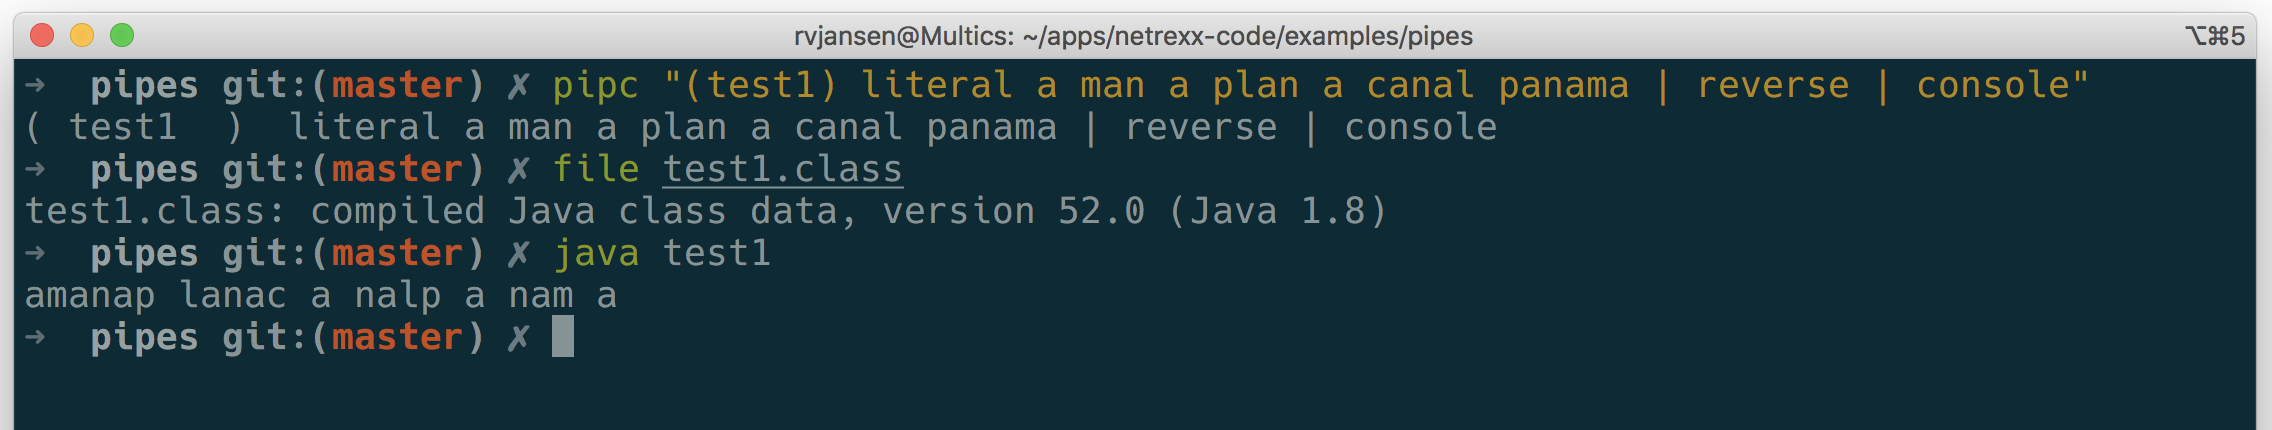
\includegraphics[width=0.75\textwidth]{images/pipcfromshell.png}
  \caption{Precompile a Pipeline from the OS command line}
  \label{fig:pipcfromshell}
\end{figure}

This will yield a \begin{alltt}test1.class\end{alltt} classfile, which
can be executed by the java virtual machine.

The file test1.class can be run with the command\footnote{or an
  appropriate shortcut in modern shells}:
\begin{verbatim}
java test1
\end{verbatim}
Be sure to leave out the .class suffix when invoking java.
% Additional options in this mode:
% Option
% Function
% Remarks
% gen	additionally save .nrx class to disk	default is -nogen
% keep	keep from the .nrx generated java source	default is -nokeep
\section{Compiled from an .njp file}
When compiled from a file, the pipe specification must not be quoted. Pipes can be specified in so-called /emph{Portrait Mode}, which is the standard for more complex pipelines as it is easier to read.
An example is:
\begin{lstlisting}
pipe (appendtest)
 
   gen 100  |
   append gen 50  |
   rexx locate /0/ |
   console
\end{lstlisting}

\section{Compiled from an .njp file with additional stage definitions in \nr{}}
An example (length1.njp) is:
\begin{lstlisting}
pipe (lengthp) < output.lst | length1 | console

import org.netrexx.njpipes.pipes.
class length1 extends stage final
  method run()
    do
      loop forever
    line = rexx peekto()
    l = line.length
    output(l l.d2x line)
    readto()
      end
    catch StageError
      rc = rc()
    end
    exit(rc*(rc<>12))
\end{lstlisting}
In this example, the name of the generated pipe is lengthp, while the name of the custom stage is length1. Be sure to invoke the right class, invoking length1 will have the JVM complain about a non-existing main method.
This class (lengthp) will be generated by the command:
\begin{verbatim}
pipc length1
\end{verbatim}
note that the .njp suffix is optional when invoking the pipes
compiler. When run, it tries to read the contents of the file
length.nrx and will put out its lines, prepended by the line length in
decimal and hex - because that is what the (in \nr{}) specified
homegrown stage does.





% \section{Building the pipeline}
% Until now everything was just theory, but now we are going to show how
% to compile and run a pipeline. The executable script \texttt{pipe} is
% included in the \nr{} distribution to specify a pipeline and to compile
% \nr{} source that contains pipelines. Pipelines can be specified on
% the command line or in a file, but will always be compiled to a .class
% file for execution in the JVM. In this case, we have the following
% pipe definition in a file called \code{firstsample.njp}. We tell the
% pipe compiler that the pipe is called \code{hello}. 
% \lstinputlisting[label=firstpipe,caption=Hello World]{firstsample.njp} 

% This specifies a pipeline consisting of a source stage
% \texttt{literal} that puts a string (``hello world'') into the pipeline, and
% a \texttt{console} sink, that puts the string on the screen. 

% We compile this pipe with the command:
% \begin{verbatim}
% pipe firstsample
% \end{verbatim} 
% \bash[stdout]
% pipc firstsample
% \END
% The pipe
% compiler will echo the source of the pipe to the screen - or issue
% messages when something was mistyped. The name of the classfile is the
% name of the pipe, here specified between parentheses. Options also go there.

% We call execute the pipe by typing:
% \begin{verbatim}
% java hello
% \end{verbatim}
% Its output is:
% \bash[stdout]
% java hello
% \END
% Now we
% have shown the obligatory example, we can make it more interesting by
% adding a \texttt{reverse} stage in between:
% \lstinputlisting[label=secondpipe,caption=Hello World 2]{secondsample.njp} 
% When this is executed, it dutifully types 
% \bash[stdout]
% pipc secondsample
% java hello2
% \END

% If we replace the string after \texttt{literal} with \texttt{arg()},
% we then can start the \texttt{hello} pipeline with a an argument to
% reverse:

% \begin{lstlisting}[label=hellopipes3,caption=Hello World3]
% pipe "(hello) literal arg() | reverse | console"
% \end{lstlisting}
%  and we run it with:
% \begin{verbatim}
% java hello a man a plan a canal panama
% \end{verbatim}
% and it will respond:
% \begin{verbatim}
% amanap lanac a nalp a nam a
% \end{verbatim}
% which goes to show that without ignoring space no palindrome is very
% convincing - which we can remedy with a change to the pipeline: use the
% \texttt{change} stage to take out the spaces:
% \begin{lstlisting}[label=hellopipes4,caption=Hello World4]
% pipe "(hello) literal arg() | change /" "// | console"
% \end{lstlisting}


\chapter{Example Session}
Imagine you have landed a job as programmer in an accounting firm,
and on your first day there is a question about backups; \emph{the backup
process takes too long}. There is an urgent need to identify the files that are produced on this day. You know how to this, of course, it is only some 20 lines of code; use the File() API, fill a collection class (you are thinking of an ArrayList already), or a TreeMap to sort the File object on last modified date already, call an instance of the Calender class, run a comparison - get that compiled and test it a bit - an hour or so would be sufficient. Of course, you need to install the Java compiler, because all machines have Java nowadays, but just not the compiler.
But if you want to really impress people, you should type in a command line and be done with it. For this you can use \nr{} pipelines. Fortunately, you emailed the \nr{}F.jar to yourself so you save it on the machine, and you're in business right away; you add it to the classpath.
Your first pipeline command should just test the waters. For this
chapter, we will use the \begin{alltt}nrws\end{alltt} program. You send a
command into the pipeline, and get its output:
\begin{lstlisting}
pipe command ls -laFTl | console
\end{lstlisting}
\begin{figure}[H]
  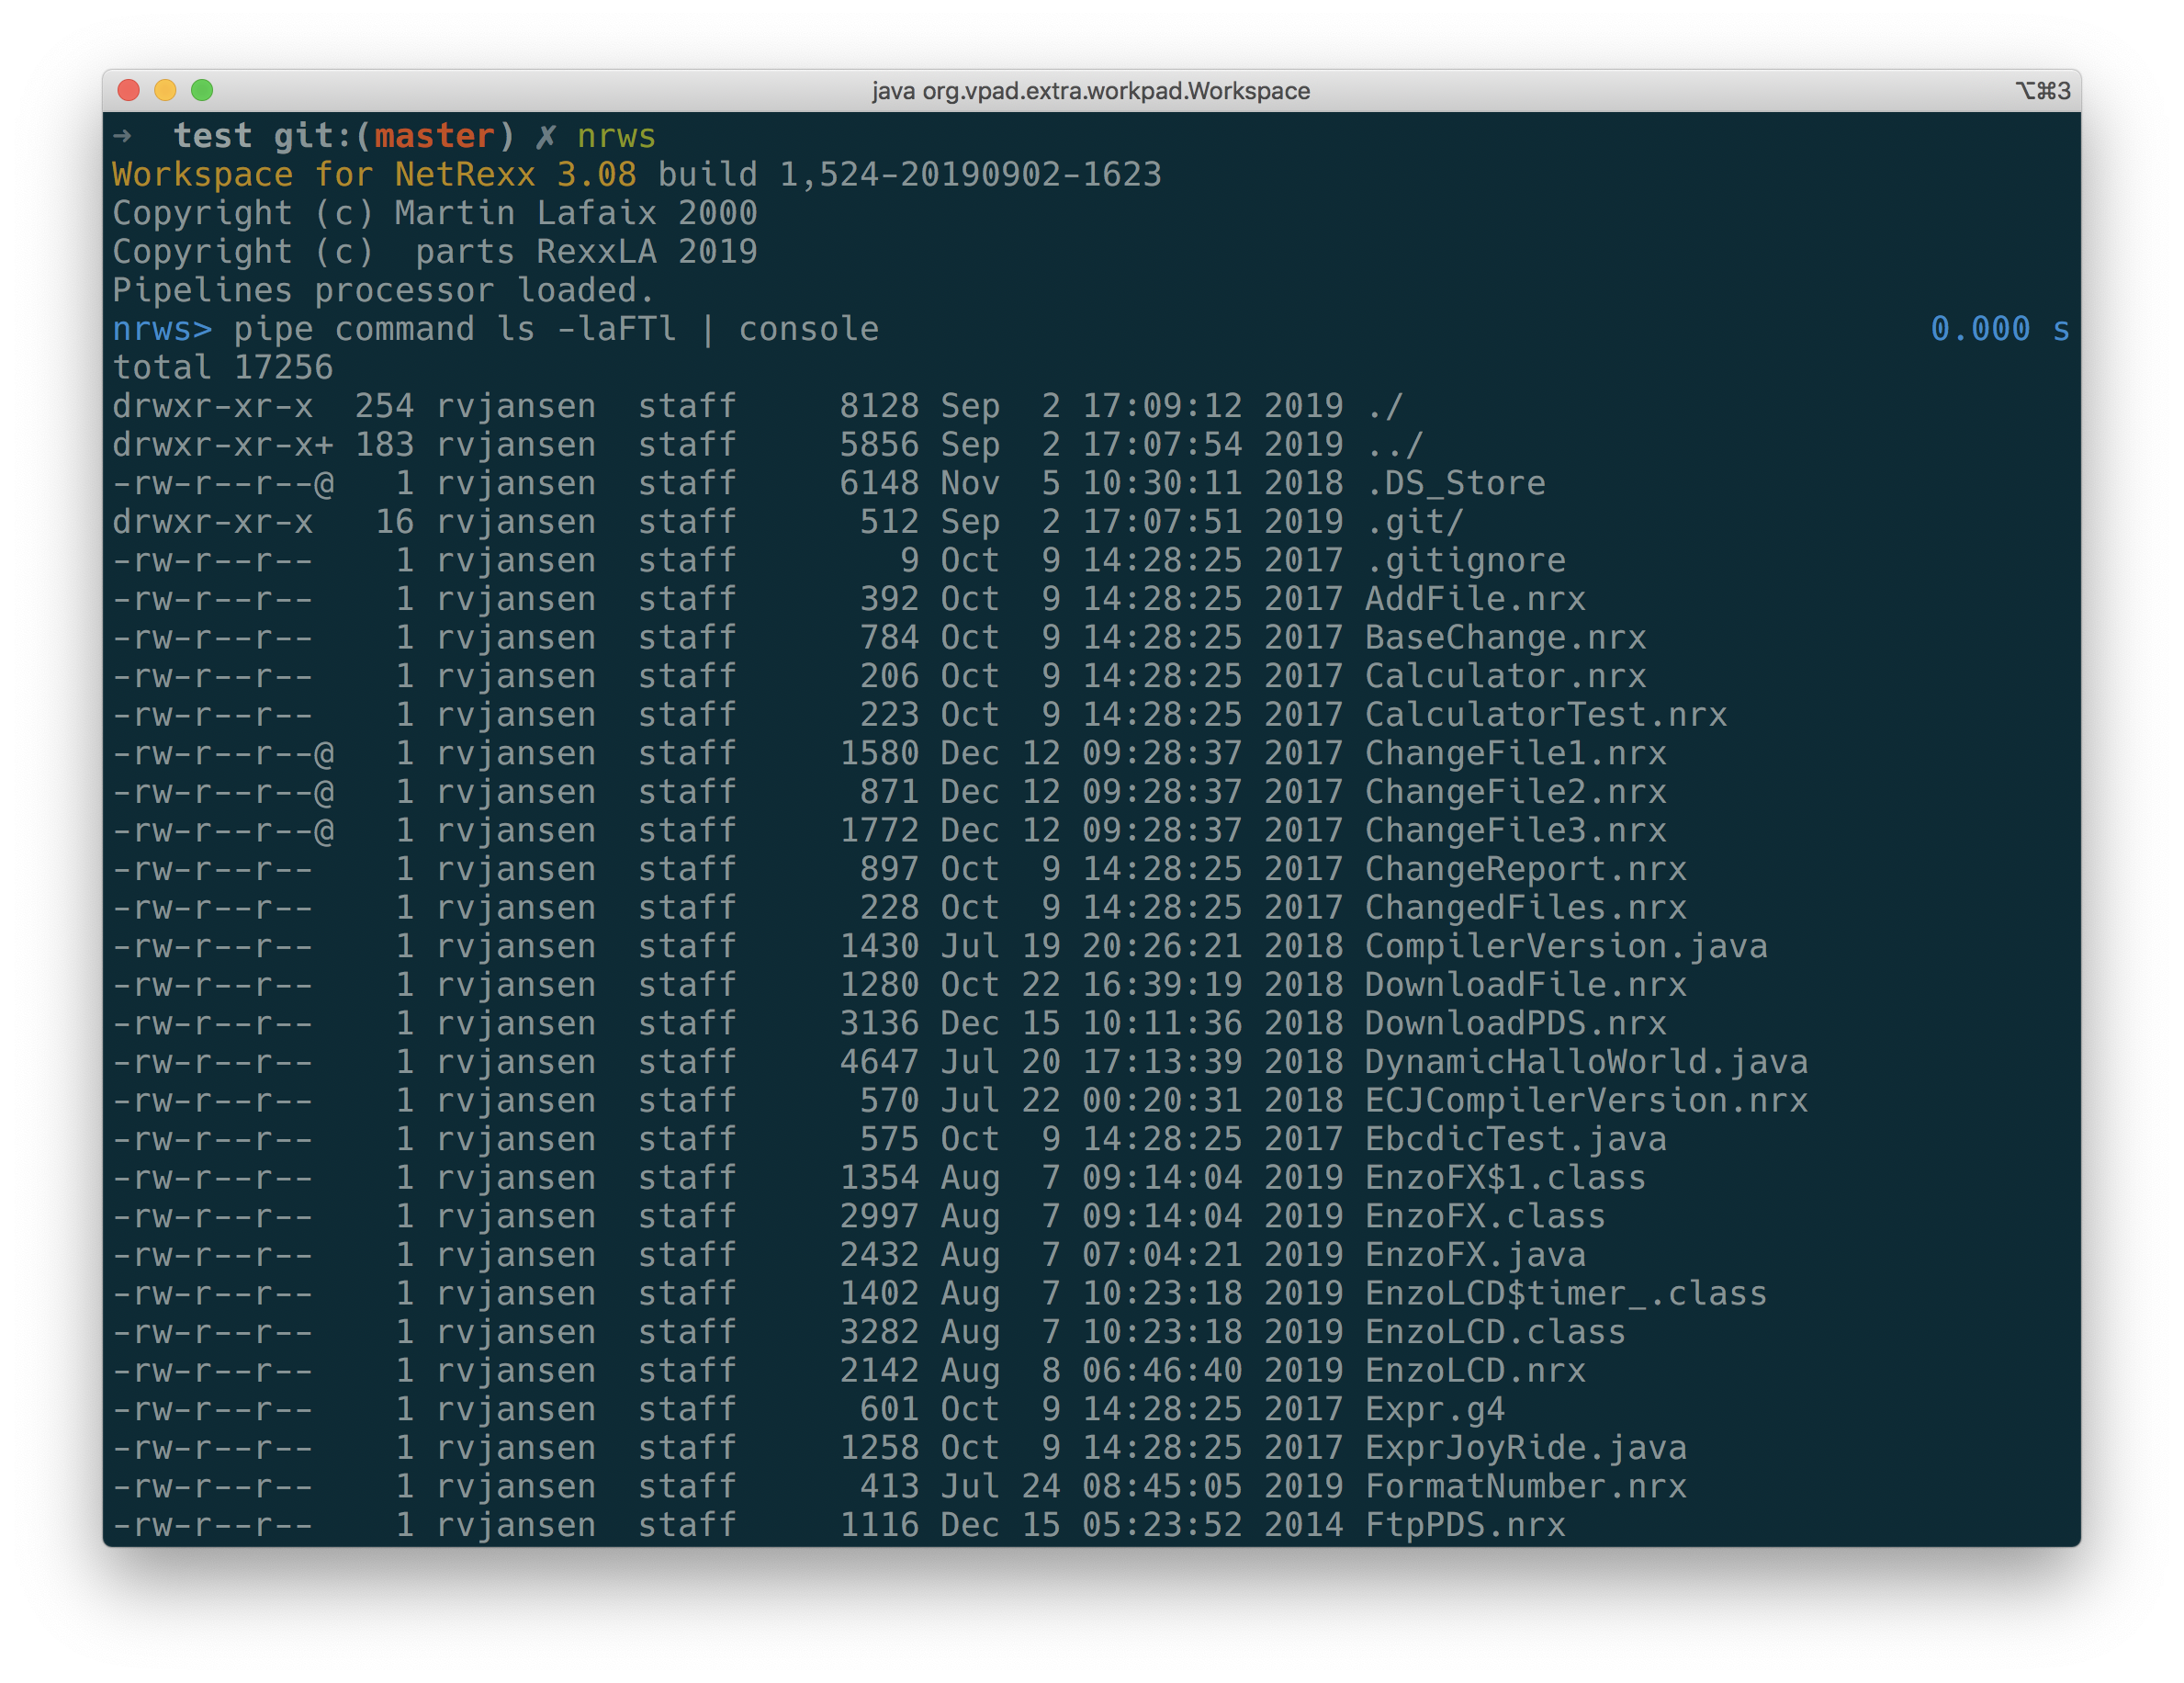
\includegraphics[width=0.75\textwidth]{images/example1.png}
  \caption{example 1}
  \label{fig:example1}
\end{figure}

The \emph{ls} command with the flags is the unix way to get a
directory listing - for Windows we would use \emph{dir}. In this case, we send the output into the pipeline, but as the last stage (called a pipe 'sink') occurs immediately after that, every line will be echoed on the console.
A number of lines like these will be displayed on the console, as in
\emph{example 1}.

You see straight away that the relevant info is not in the first
columns, and not in consecutive columns; we want to know the date
(whether it is today or not) and not the time. So we filter this out
of every line with a \texttt{specs} stage, as in \emph{example 2}.
\begin{lstlisting}
pipe command ls -laFTl | specs 42-47 1 58-* 8 | console
\end{lstlisting}
\begin{figure}[h]
  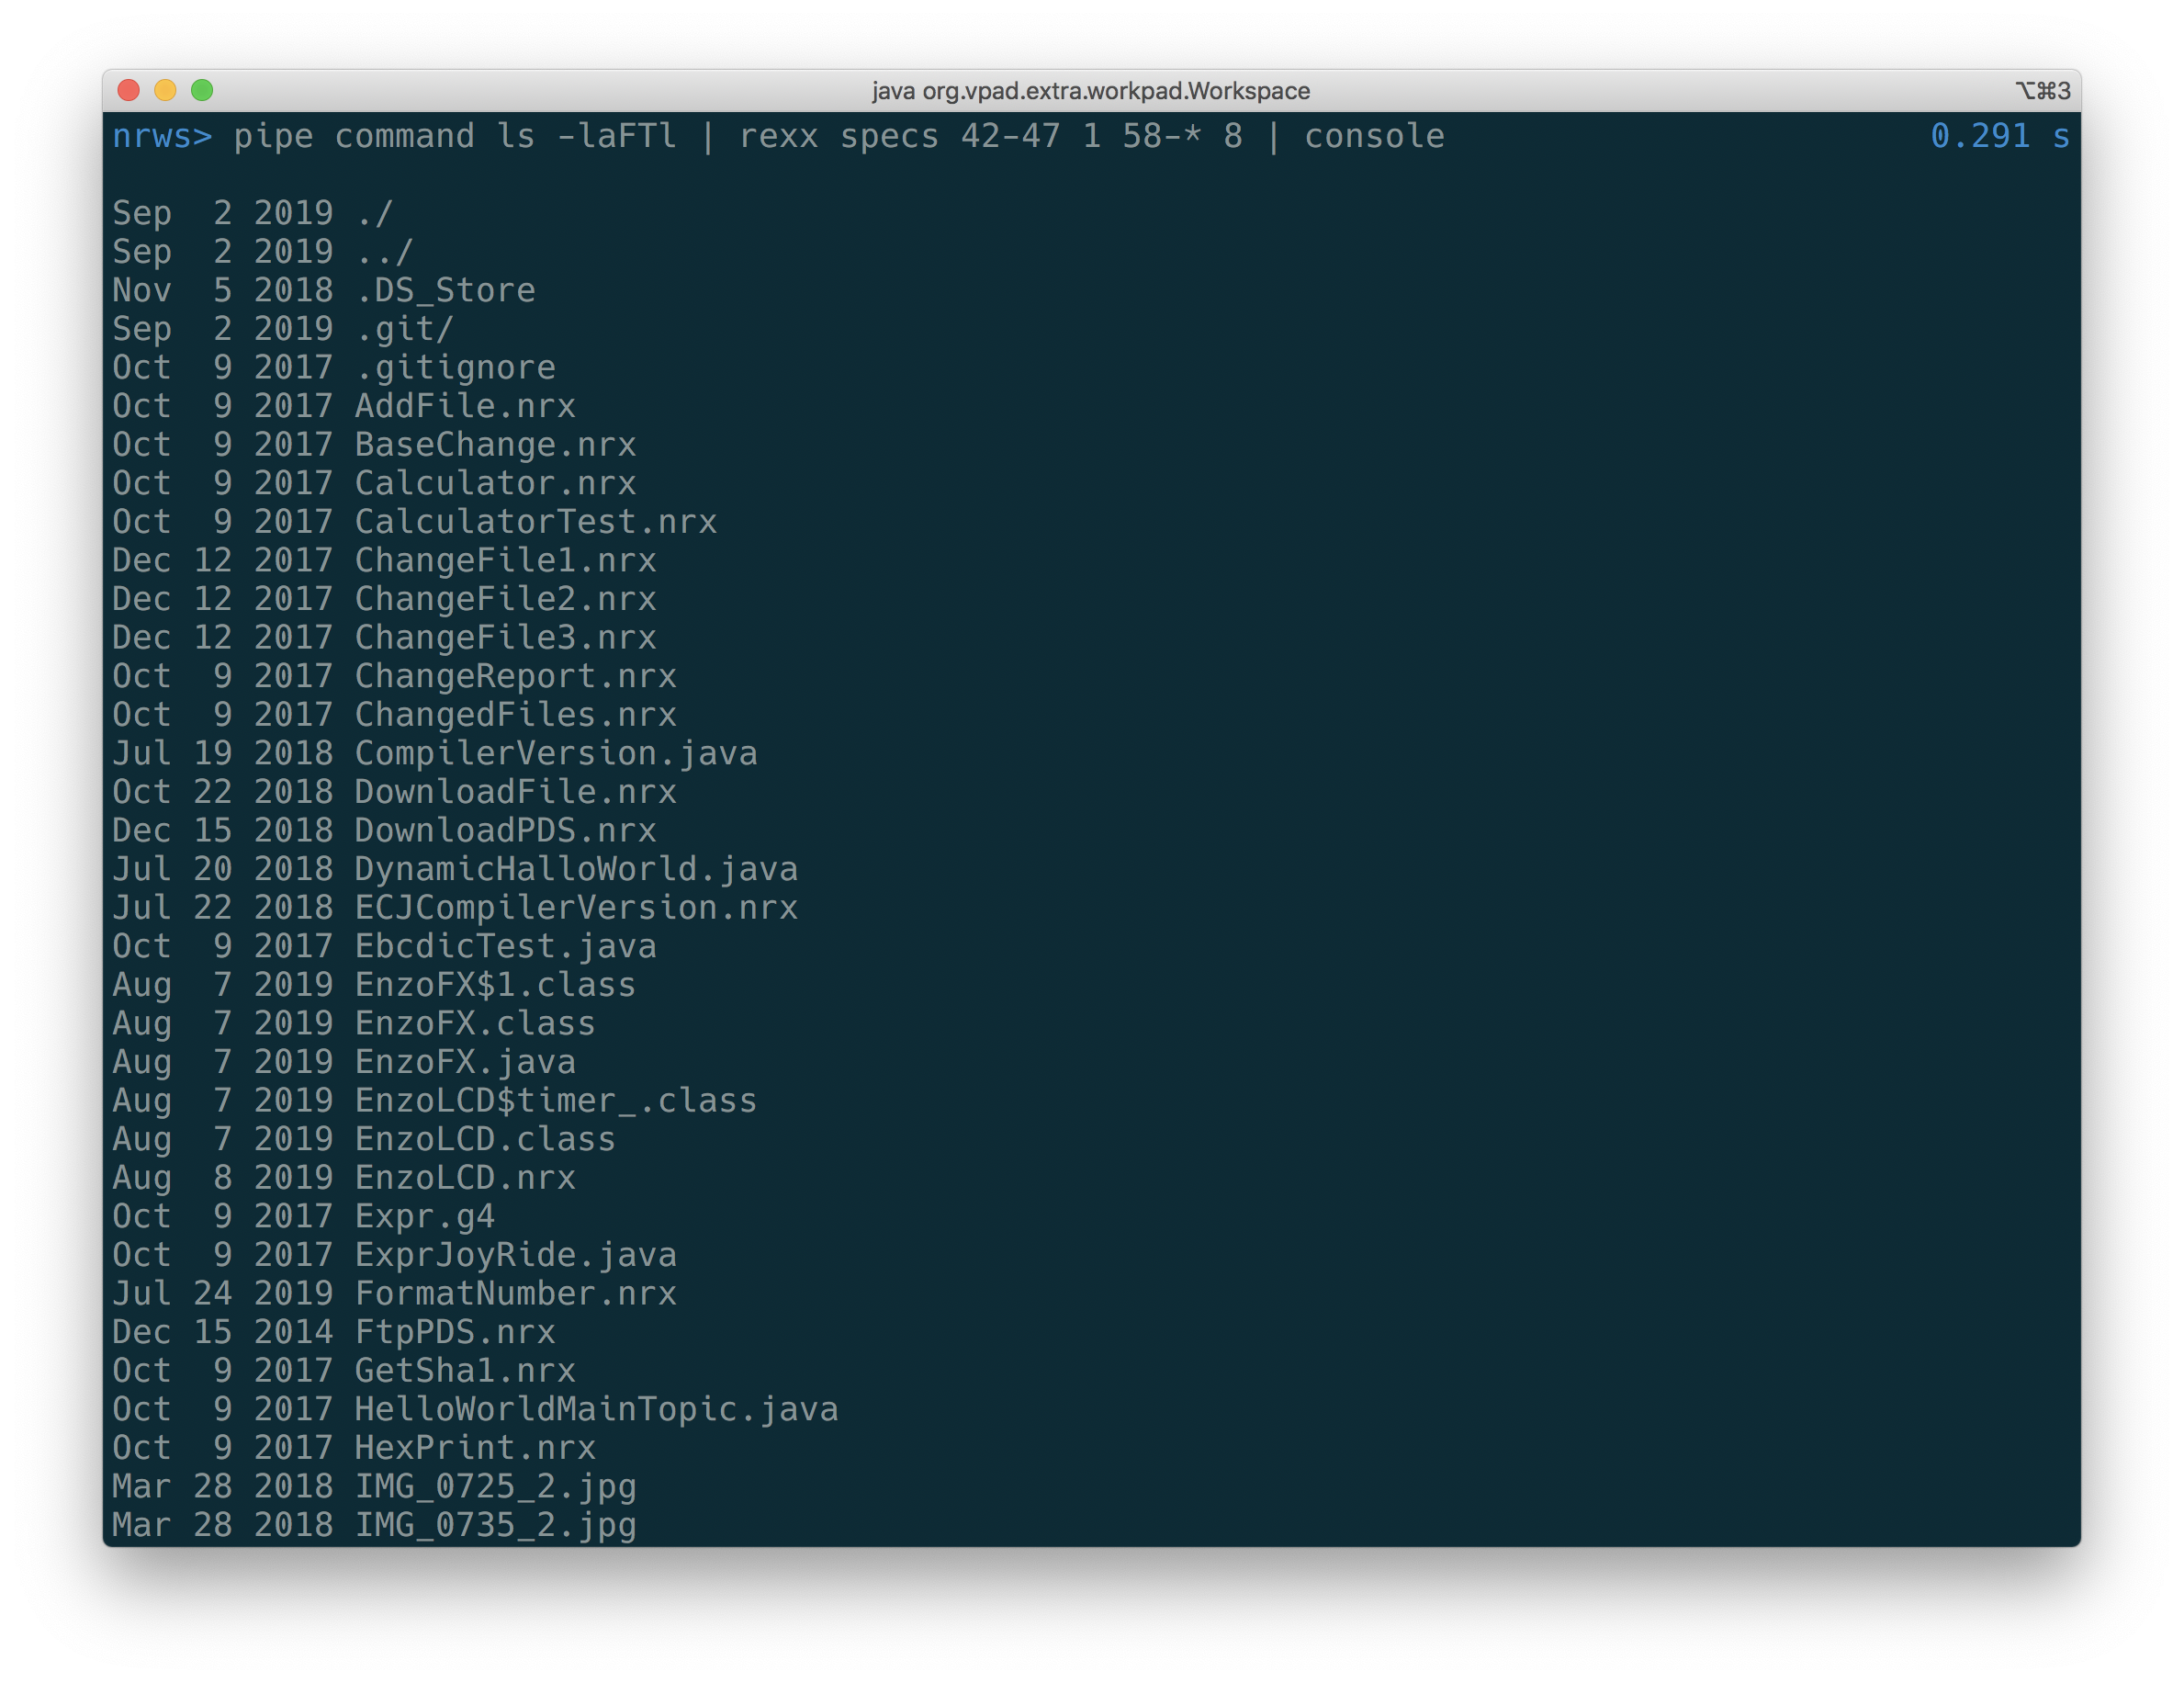
\includegraphics[width=0.75\textwidth]{images/example2.png}
  \caption{example 2}
  \label{fig:example2}
\end{figure}
We can easily sort this, with almost no programming:
\begin{lstlisting}
pipe command ls -laFTl | specs 42-47 1 58-* 8 | sort | console
\end{lstlisting}
So what now comes out of the pipeline is sorted (see \emph{example 3}).
But this is a bit funny, we would like to see chronological order of course, so we switch around some columns with another specs stage:
\begin{figure}[h]
  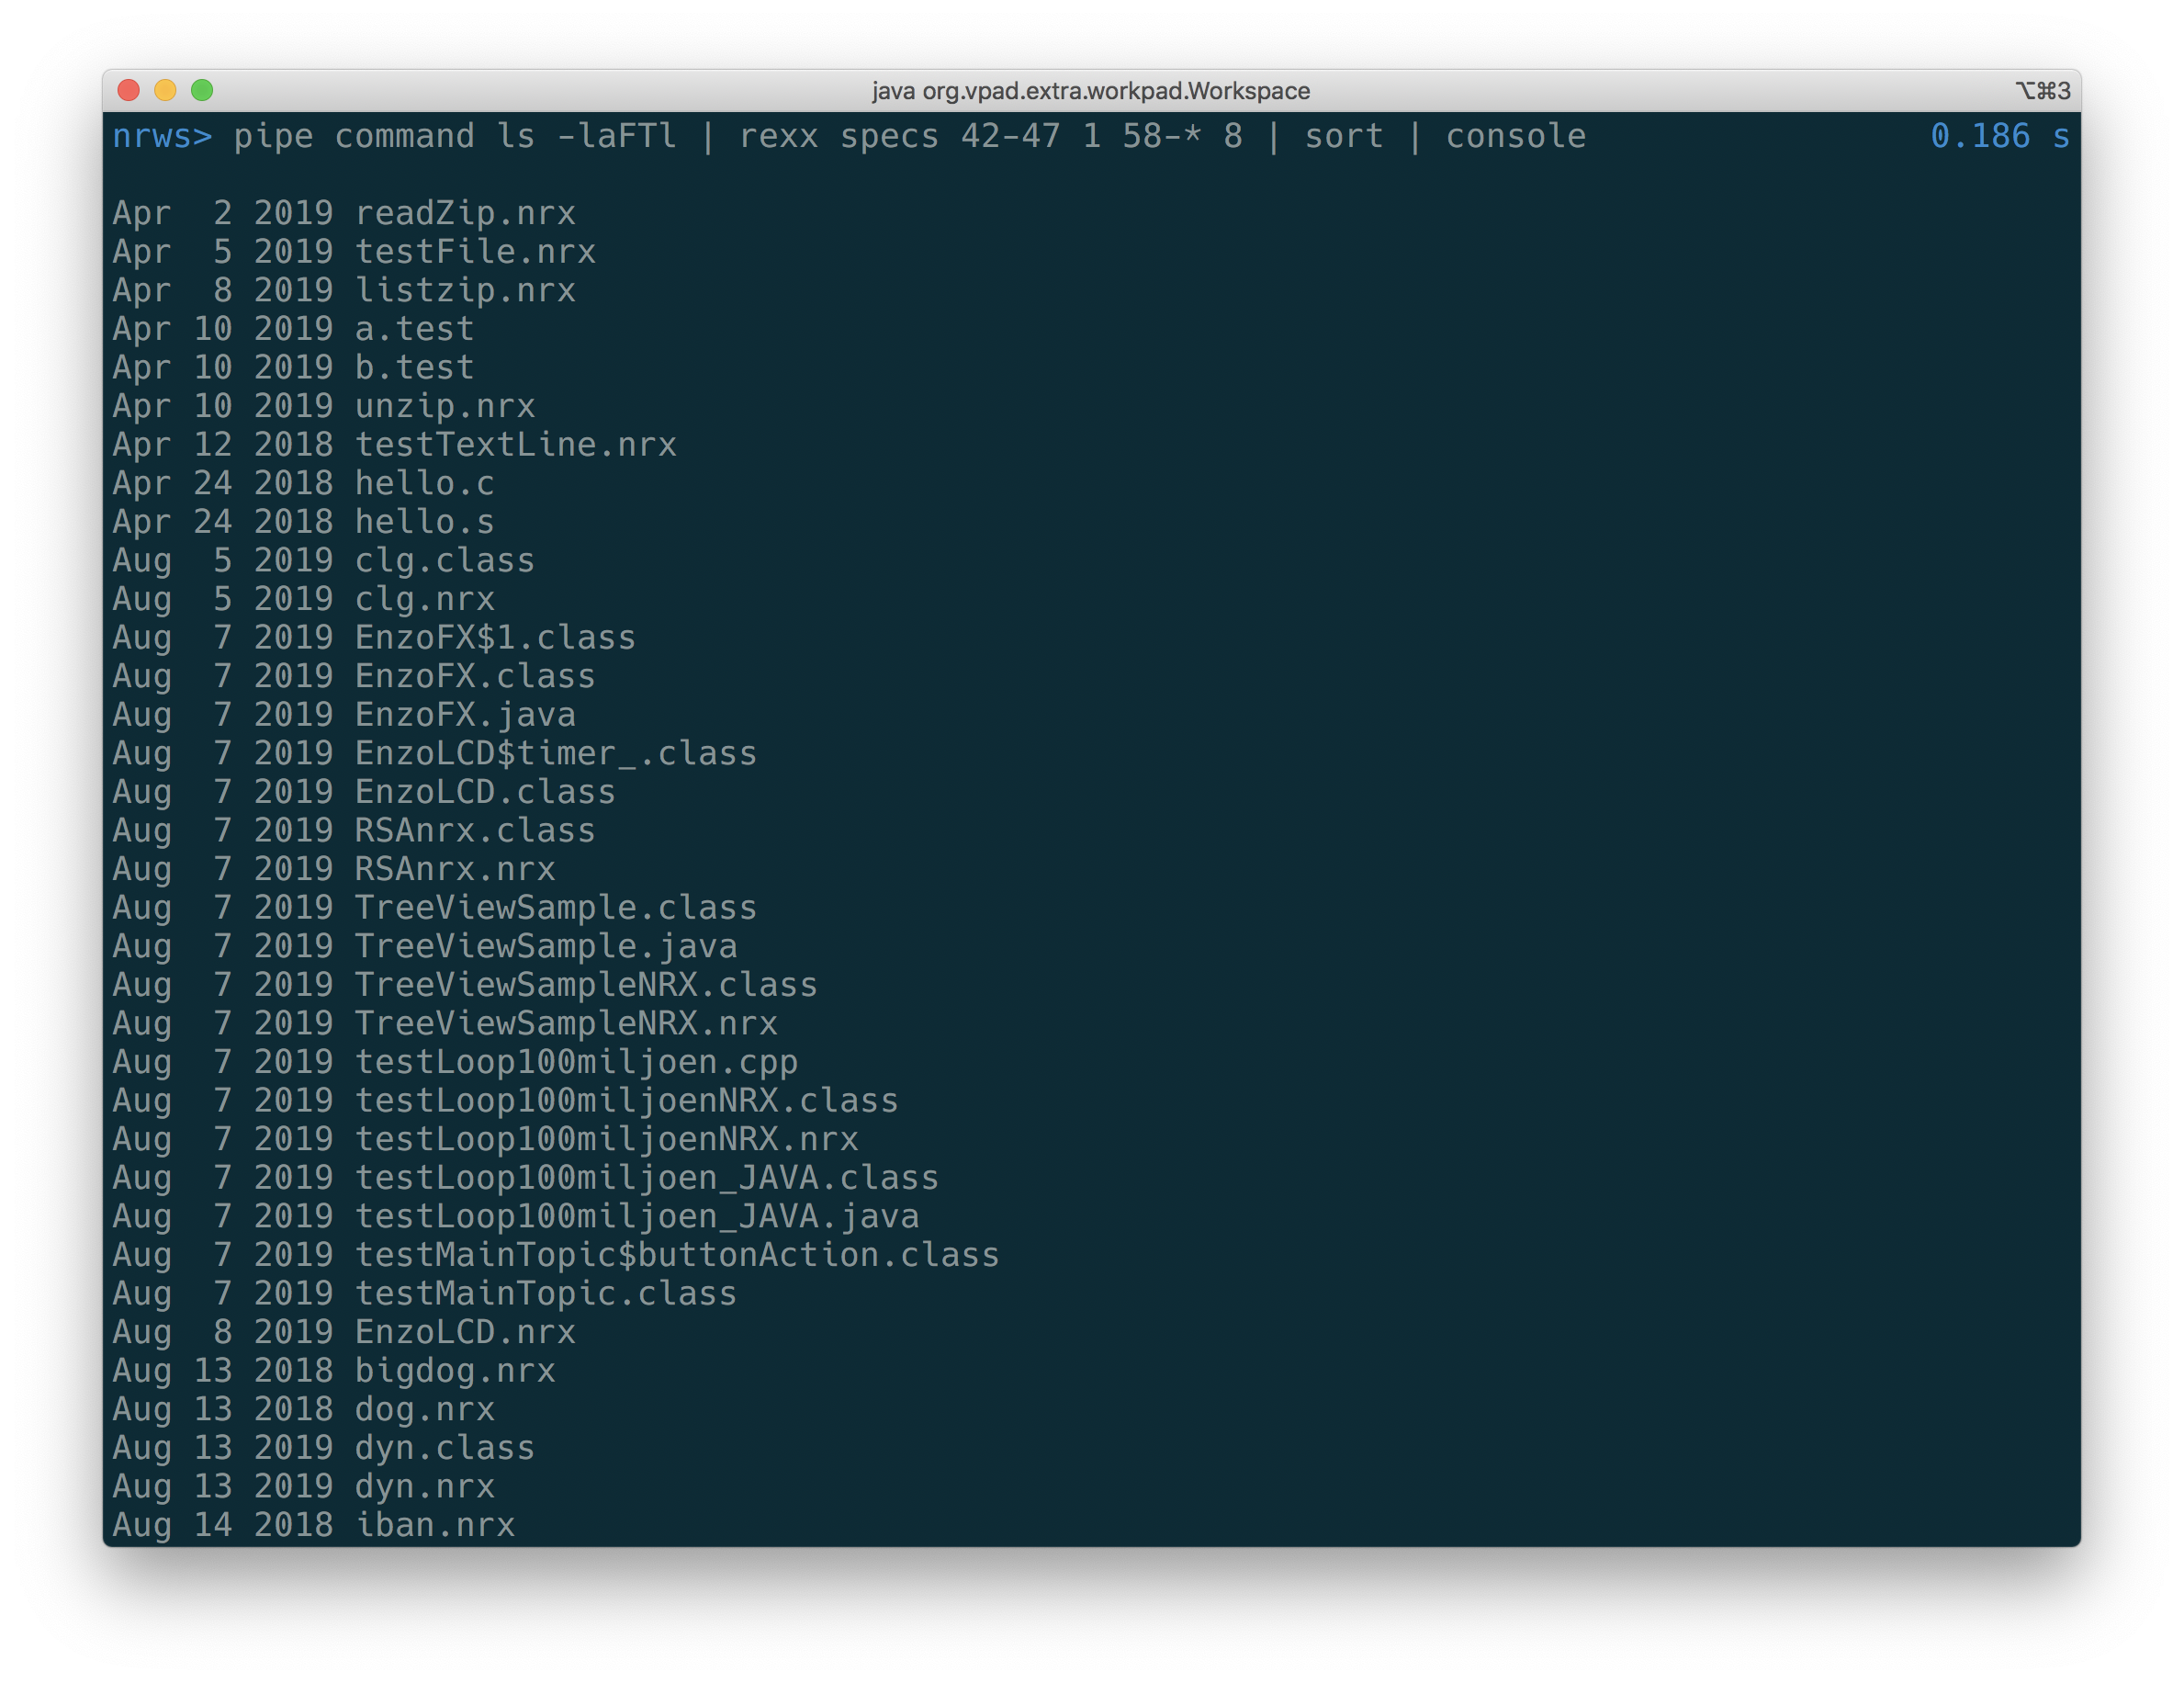
\includegraphics[width=0.75\textwidth]{images/example3.png}
  \caption{example 3}
  \label{fig:example3}
\end{figure}
\begin{lstlisting}
pipe command ls -laFTl | specs 42-47 1 58-* 8 | specs 7-11 1 1-6 7 12-* 12 | sort | console
\end{lstlisting}
\begin{figure}[h]
  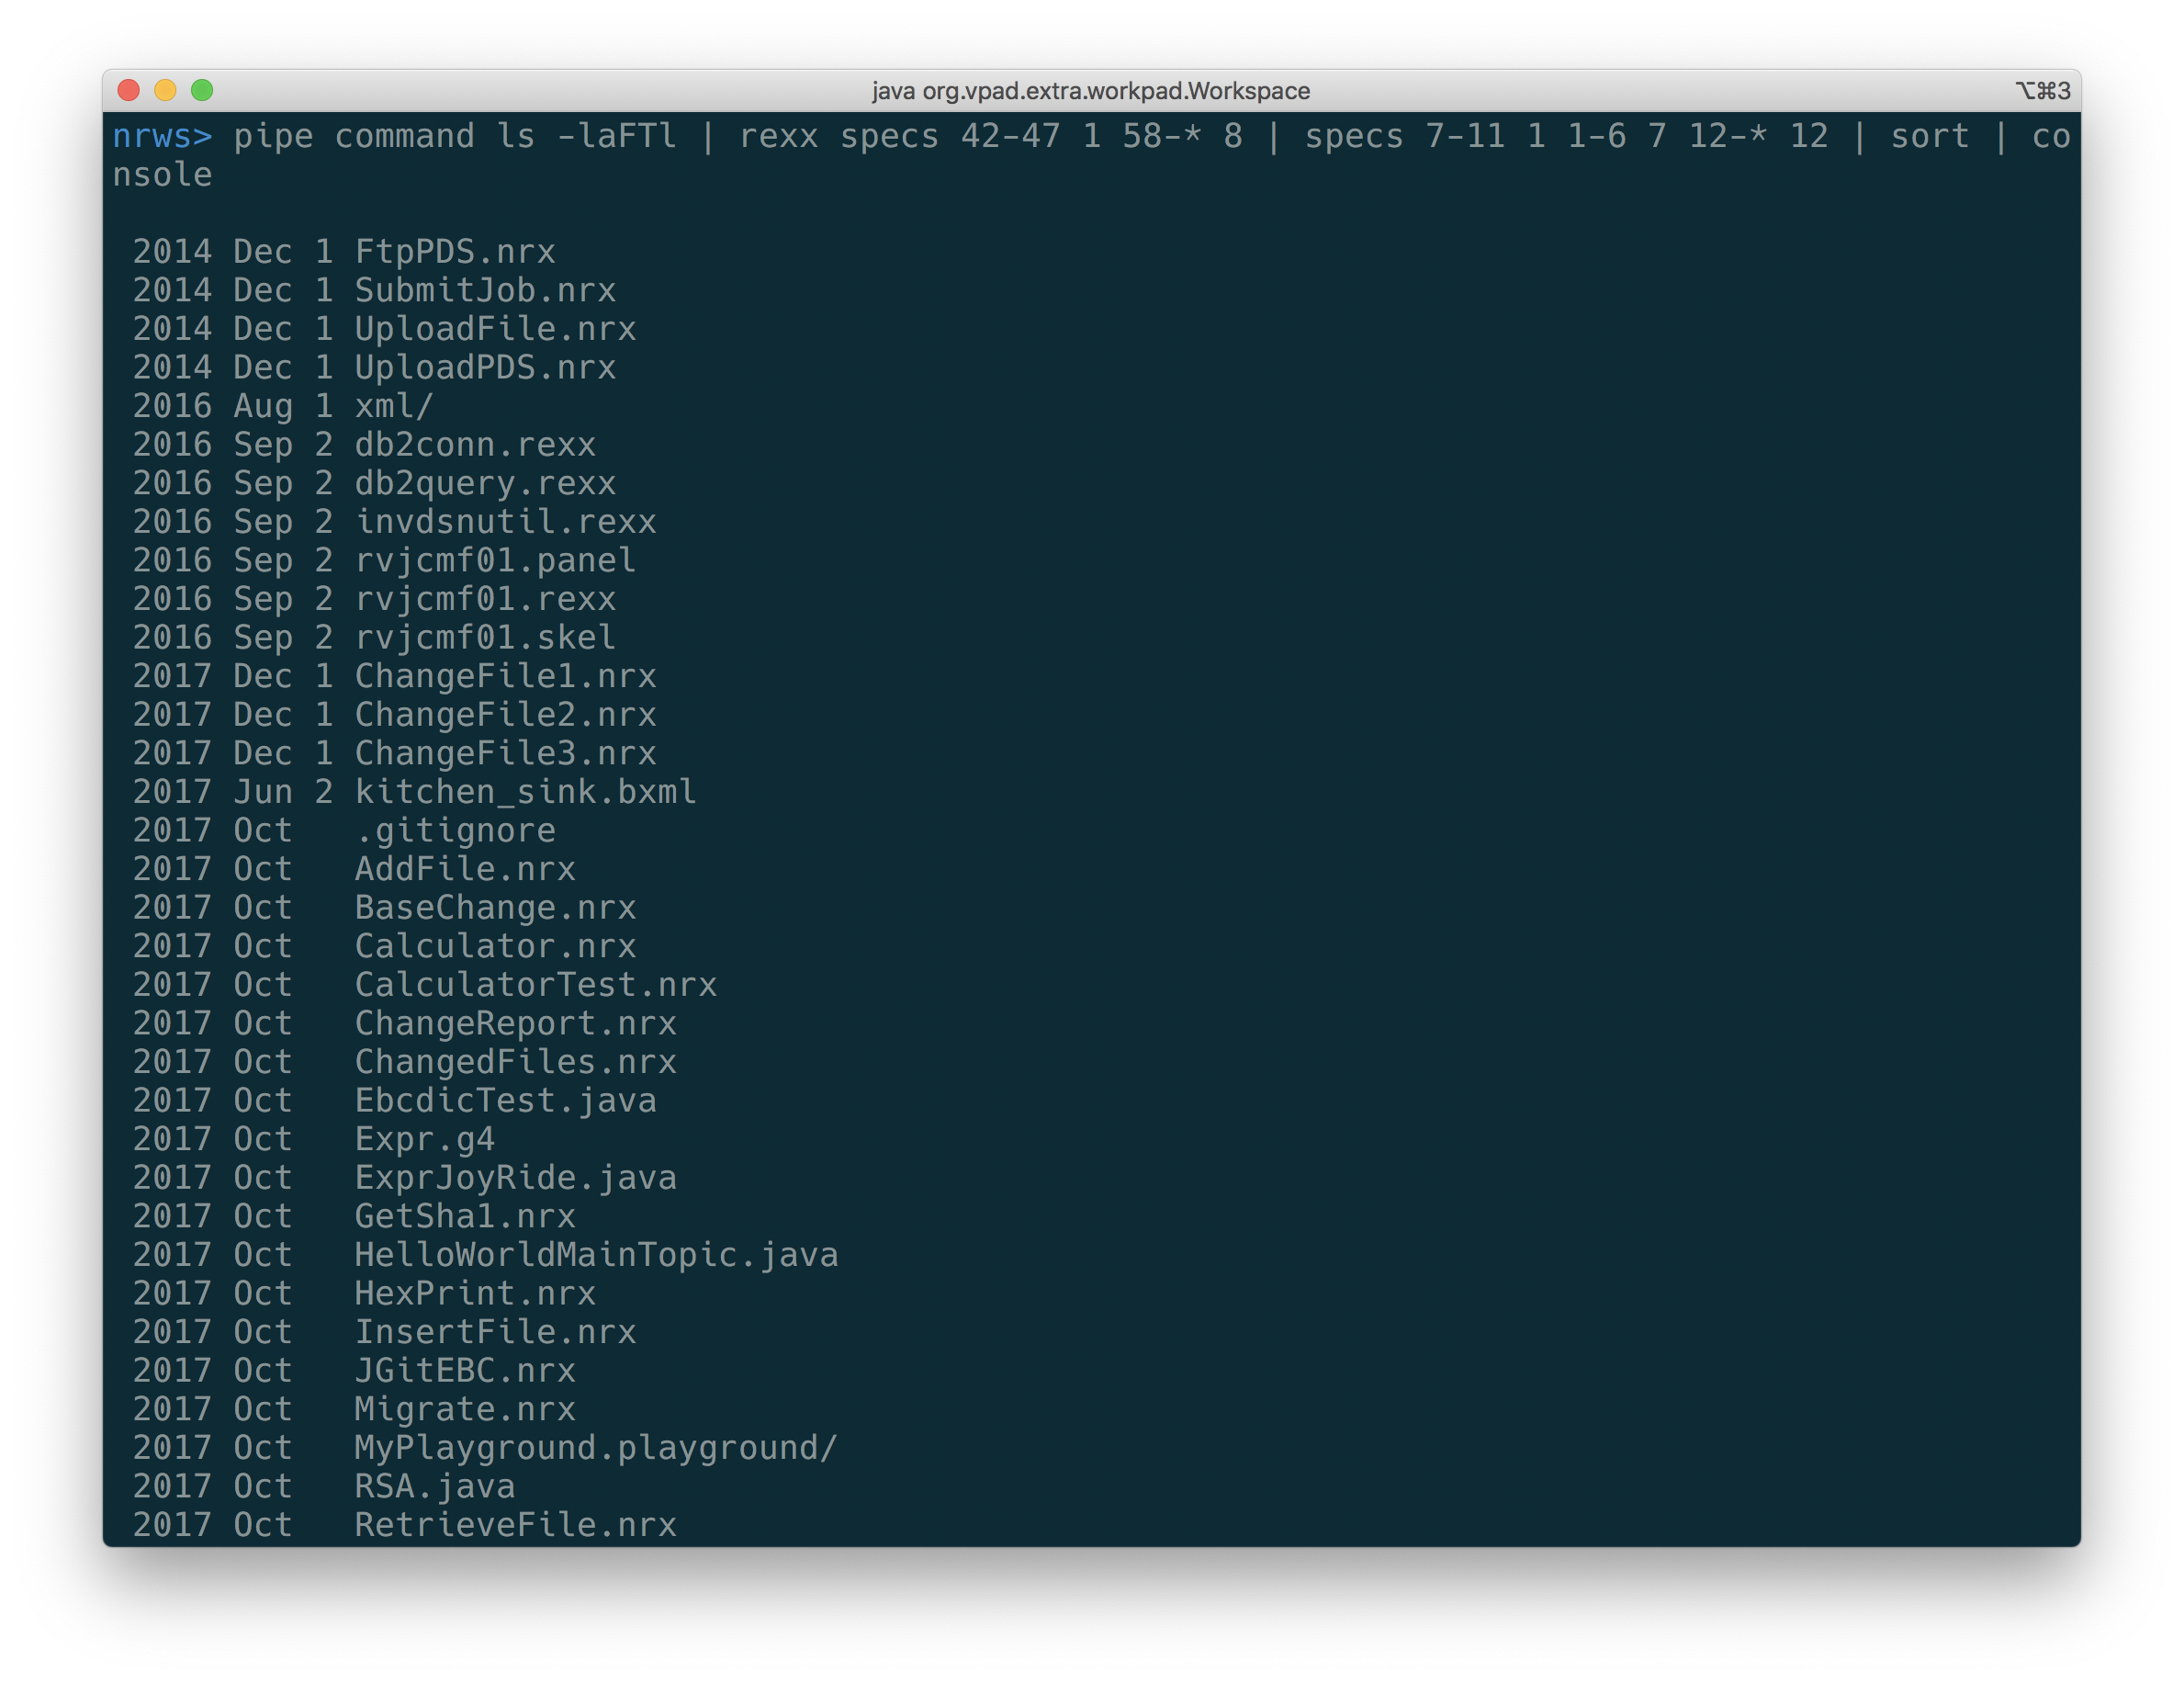
\includegraphics[width=0.75\textwidth]{images/example4.png}
  \caption{example 4}
  \label{fig:example4}
\end{figure}
which is very near to what we want (see \emph{example 4}). Only thing to do now is to filter
on the date. We use the \emph{locate} stage and hardcode the date for
now. Let's say it is the 2nd of March, 2019:
\begin{lstlisting}
pipe command ls -laFTl | specs 42-47 1 58-* 8 |  specs 7-11 1 1-6
7 12-* 12 | locate /2019 Mar 2/ | sort | console
\end{lstlisting}
\begin{figure}[h]
  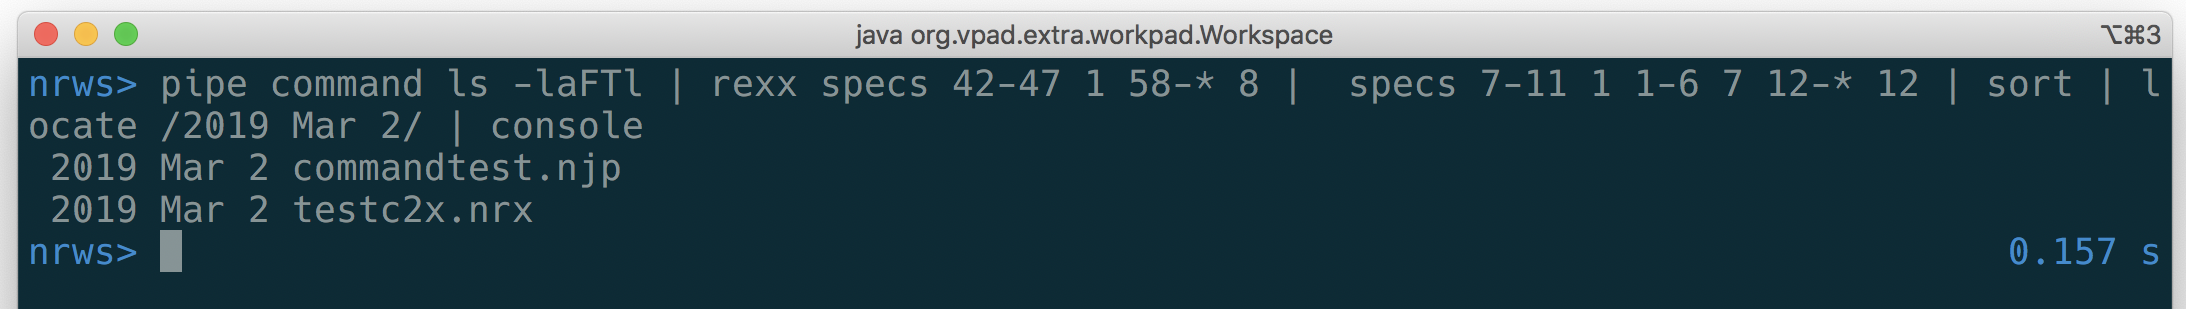
\includegraphics[width=0.75\textwidth]{images/example5.png}
  \caption{example 5}
  \label{fig:example5}
\end{figure}
As \emph{example 5} shows, on that day there were only two files
produced. Also, because this is a short list now, you can see that
Pipelines runs this pipe in 0.157 seconds, because we switched on the
time option in \emph{nrws}.
Normally, you would specify your pipeline in a file and use
\emph{portrait mode}:
commandtest.njp:
\begin{lstlisting}
pipe (newfiles)
command ls -laFTl |
specs 42-47 1 58-* 8 |
specs 7-11 1 1-6 7 12-* 12 |
sort |
locate /2019 Mar 2/ |
console
\end{lstlisting}
The filename is different from the generated class file name, on purpose. You could, and would, put different related pipelines in one file.
Then we do a:
\begin{alltt}
pipc commandtest && java newfiles
\end{alltt}

\chapter{Write your own Filters}
So we have seen in the previous example that it is not too hard to
make a simple pipeline out of things called 'device drivers' (such as
\emph{command}, for OS commands, '<' for reading files on disk, and
\emph{literal}, for inserting literal strings into a pipeline,
filters, and sinks.
% We received some comments, here and on the CMS-Pipelines list, that the first example was too easy and more representative for Unix pipes than for VM, which can do more involved multistream stuff. That is true, but we would like to start with the easier examples so everybody is still comfortable. So please hold your horses while I show you something that is also really cool. And please try the things we showed with the spec stages in a Unix pipe: you'll probably need awk to do that and it will not be as clean as the specs examples, so it is not that easy; writing a Unix filter in C is even more work.
% One of the most appealing characteristics of piping on CMS and TSO is
% that you can make your own filters in Rexx, and that it is really
% simple. Of course, this also works in \nr{} and its Pipelines
% implementation.
When a filter is not delivered in the standard set of stages, it is
very easy to make one yourself in the \nr{} language. The model for
this closely follows the way it is done with CMS Pipelines and Classic
Rexx.
Imagine, for the sake of argument (and a simple example\footnote{From
the document CMS Pipelines Explained, by John P. Hartmann}), that you have an
assignment to quickly reverse a string.
\begin{lstlisting}
  /* BAGVENDT REXX -- Reverse the contents of lines in the pipeline    */
signal on error
 do forever
   'peekto data'
   'output' reverse(data)
   'readto'
end
error: exit RC*(RC<>12)
\end{lstlisting}
And you would need to remember to call your filetype REXX instead of EXEC.  The \texttt{peekto} reads the input but does not actually commit the read yet, so you can read it one more time with knowledge about the contents. The \texttt{output} pushes its argument back into the pipeline. The \texttt{readto} reads and commits the read so the line is really processed and we can go to the next one.

In \nr{}, that would be about the same, but for some small changes
incurred by the object oriented model of \nr{}, which does not exist in Classic Rexx. Here \texttt{peekto()}, \texttt{readto()} and
\texttt{output()} are method calls on the \texttt{stage} object. This
will be made addressable
by the import from org.netrexx.njpipes.pipes. (file: \texttt{bagvendt.nrx})
\begin{lstlisting}
import org.netrexx.njpipes.pipes.
class bagvendt extends stage
method run()
   loop forever
      line = Rexx peekto()
      output(line.reverse())
      readto()
   catch StageError
      rc = rc()
   end
exit(rc*(rc<>12))
\end{lstlisting}
So that would look fairly familiar, and admittedly, a bit easier for us already well versed in \nr{}.
We can test this by building a pipeline and running the filter on its
own source:
\begin{alltt}
pipe "literal abcd | bagvendt | console"
 \end{alltt}
If you have a CMS handy, that would be:
\begin{alltt}
pipe literal abcd | bagvendt | console
 \end{alltt}
on the first, Classic Rexx version of the filter - but the quoted
version also works on CMS.
\begin{figure}[h]
  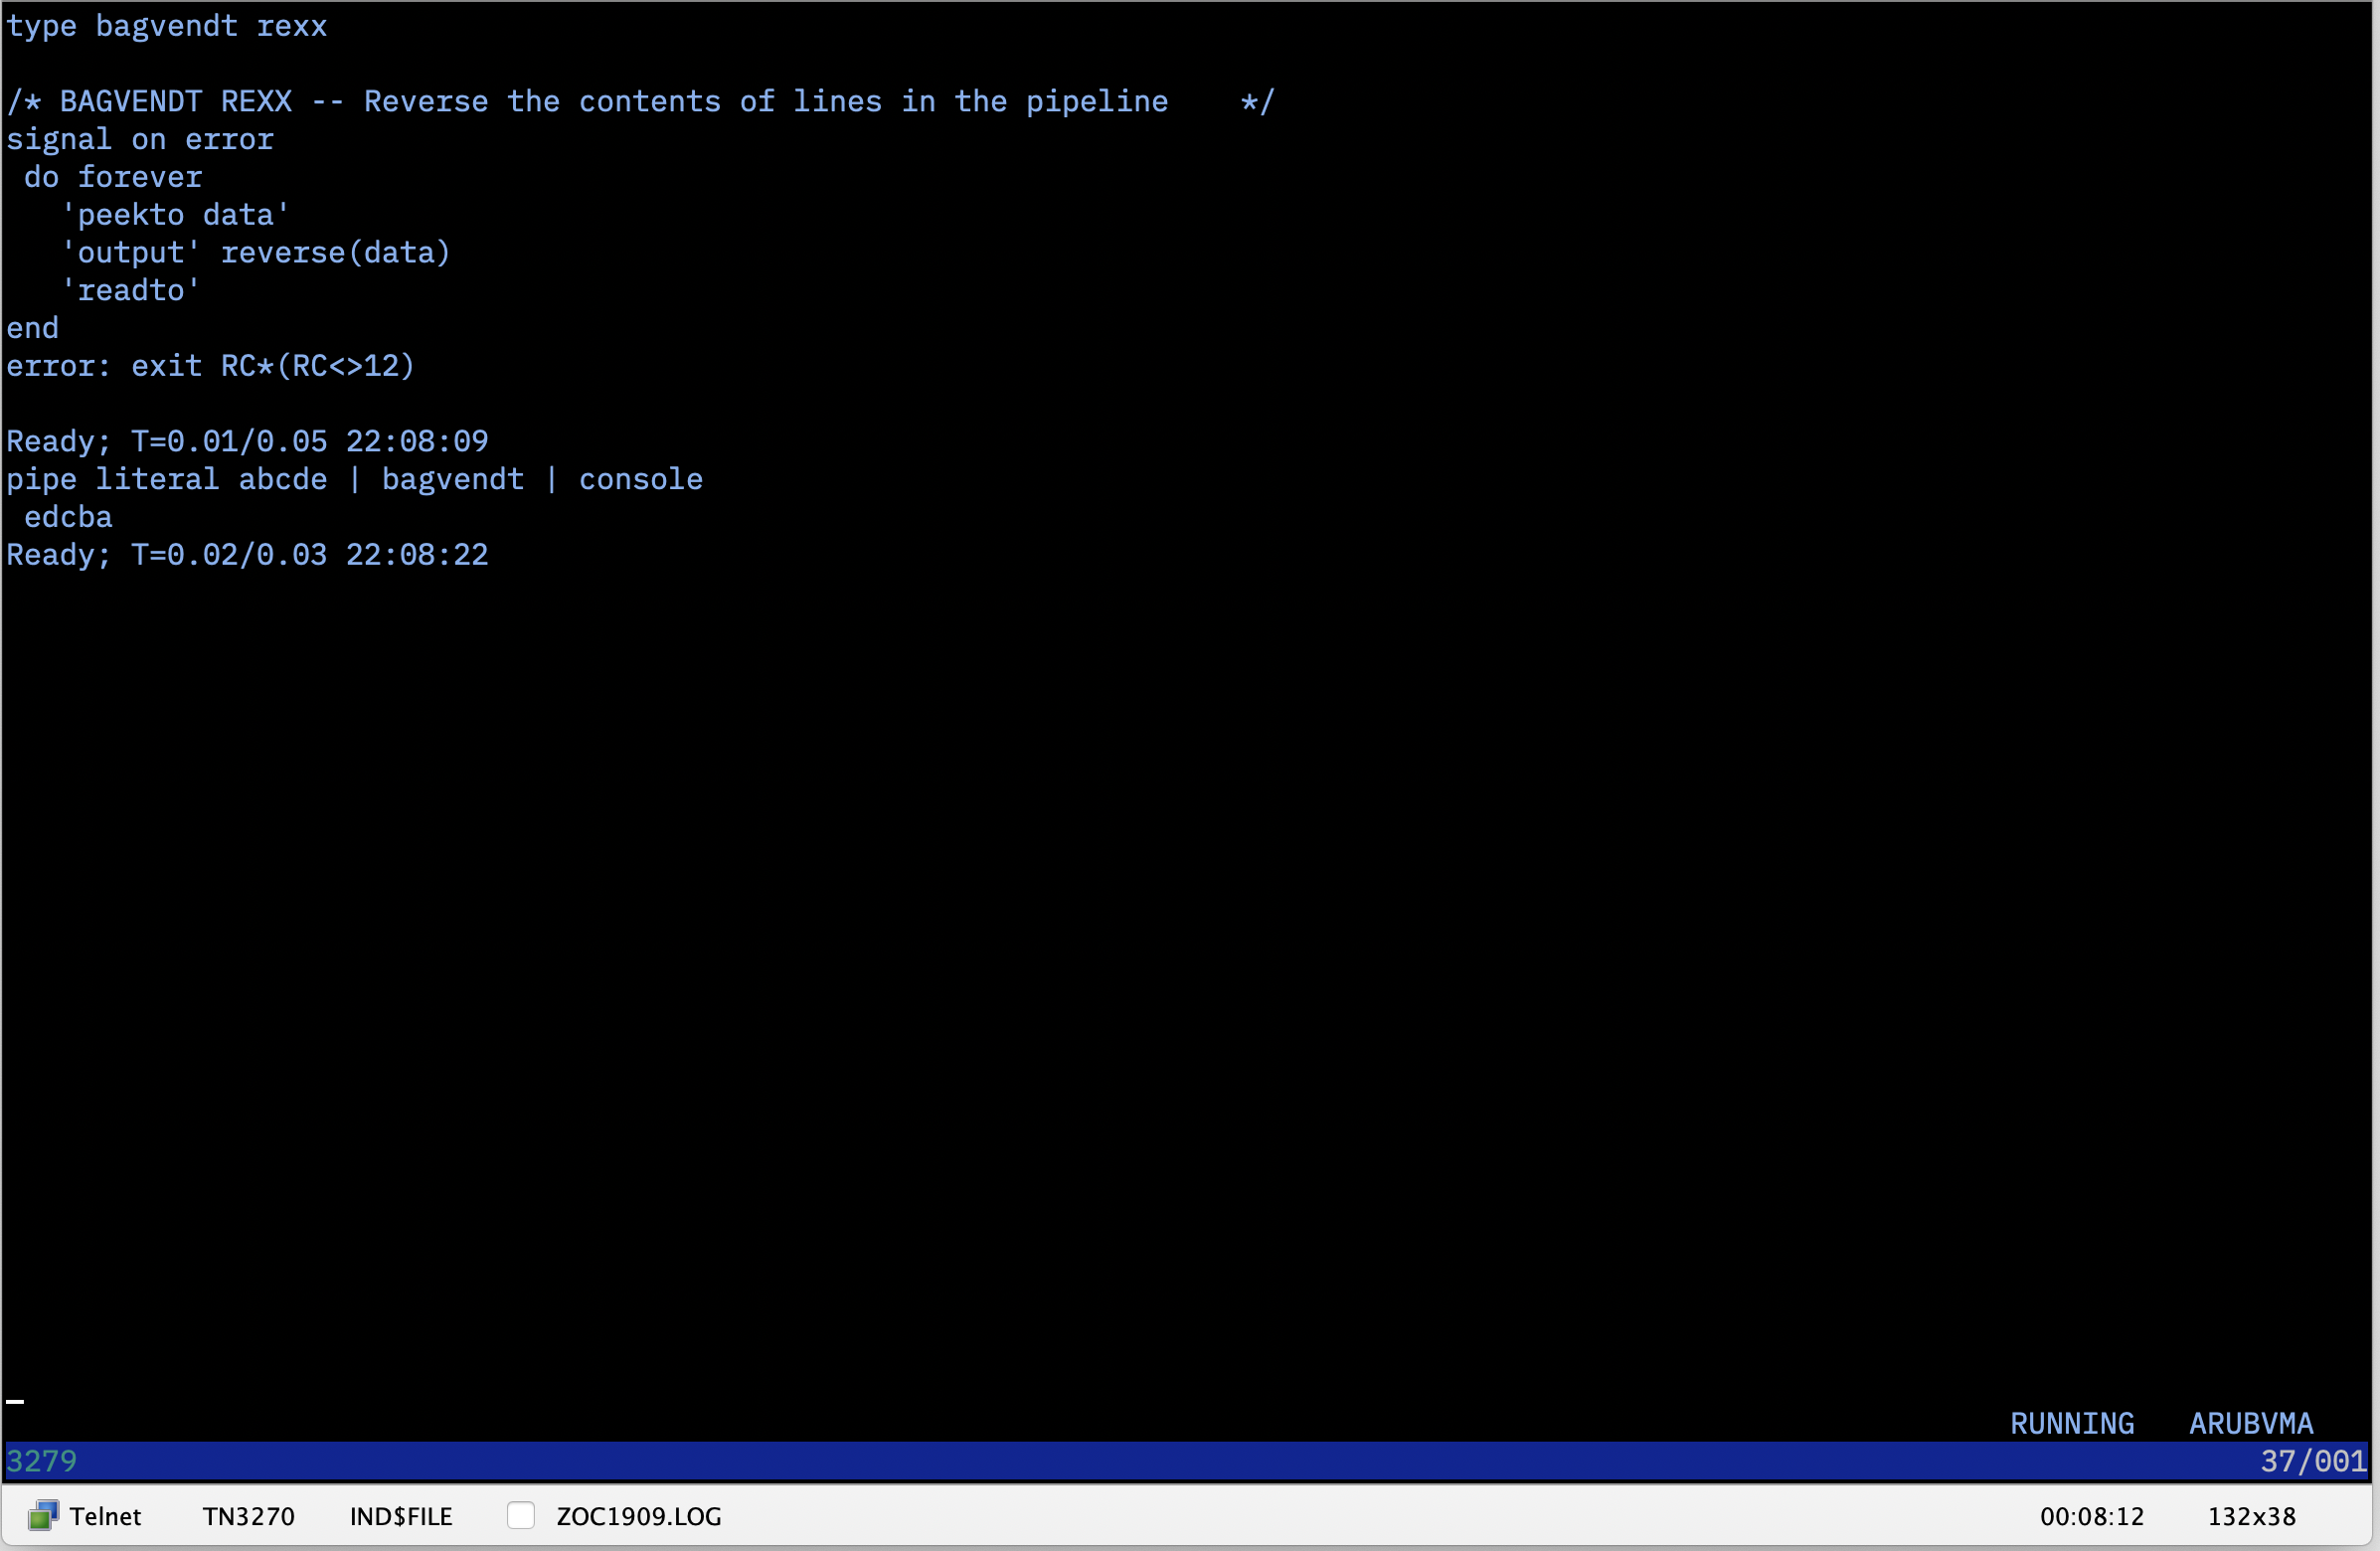
\includegraphics[width=0.75\textwidth]{images/vmbagvendt.png}
  \caption{BAGVENDT under VM/CMS}
  \label{fig:vmbagvendt}
\end{figure}\begin{figure}[h]
  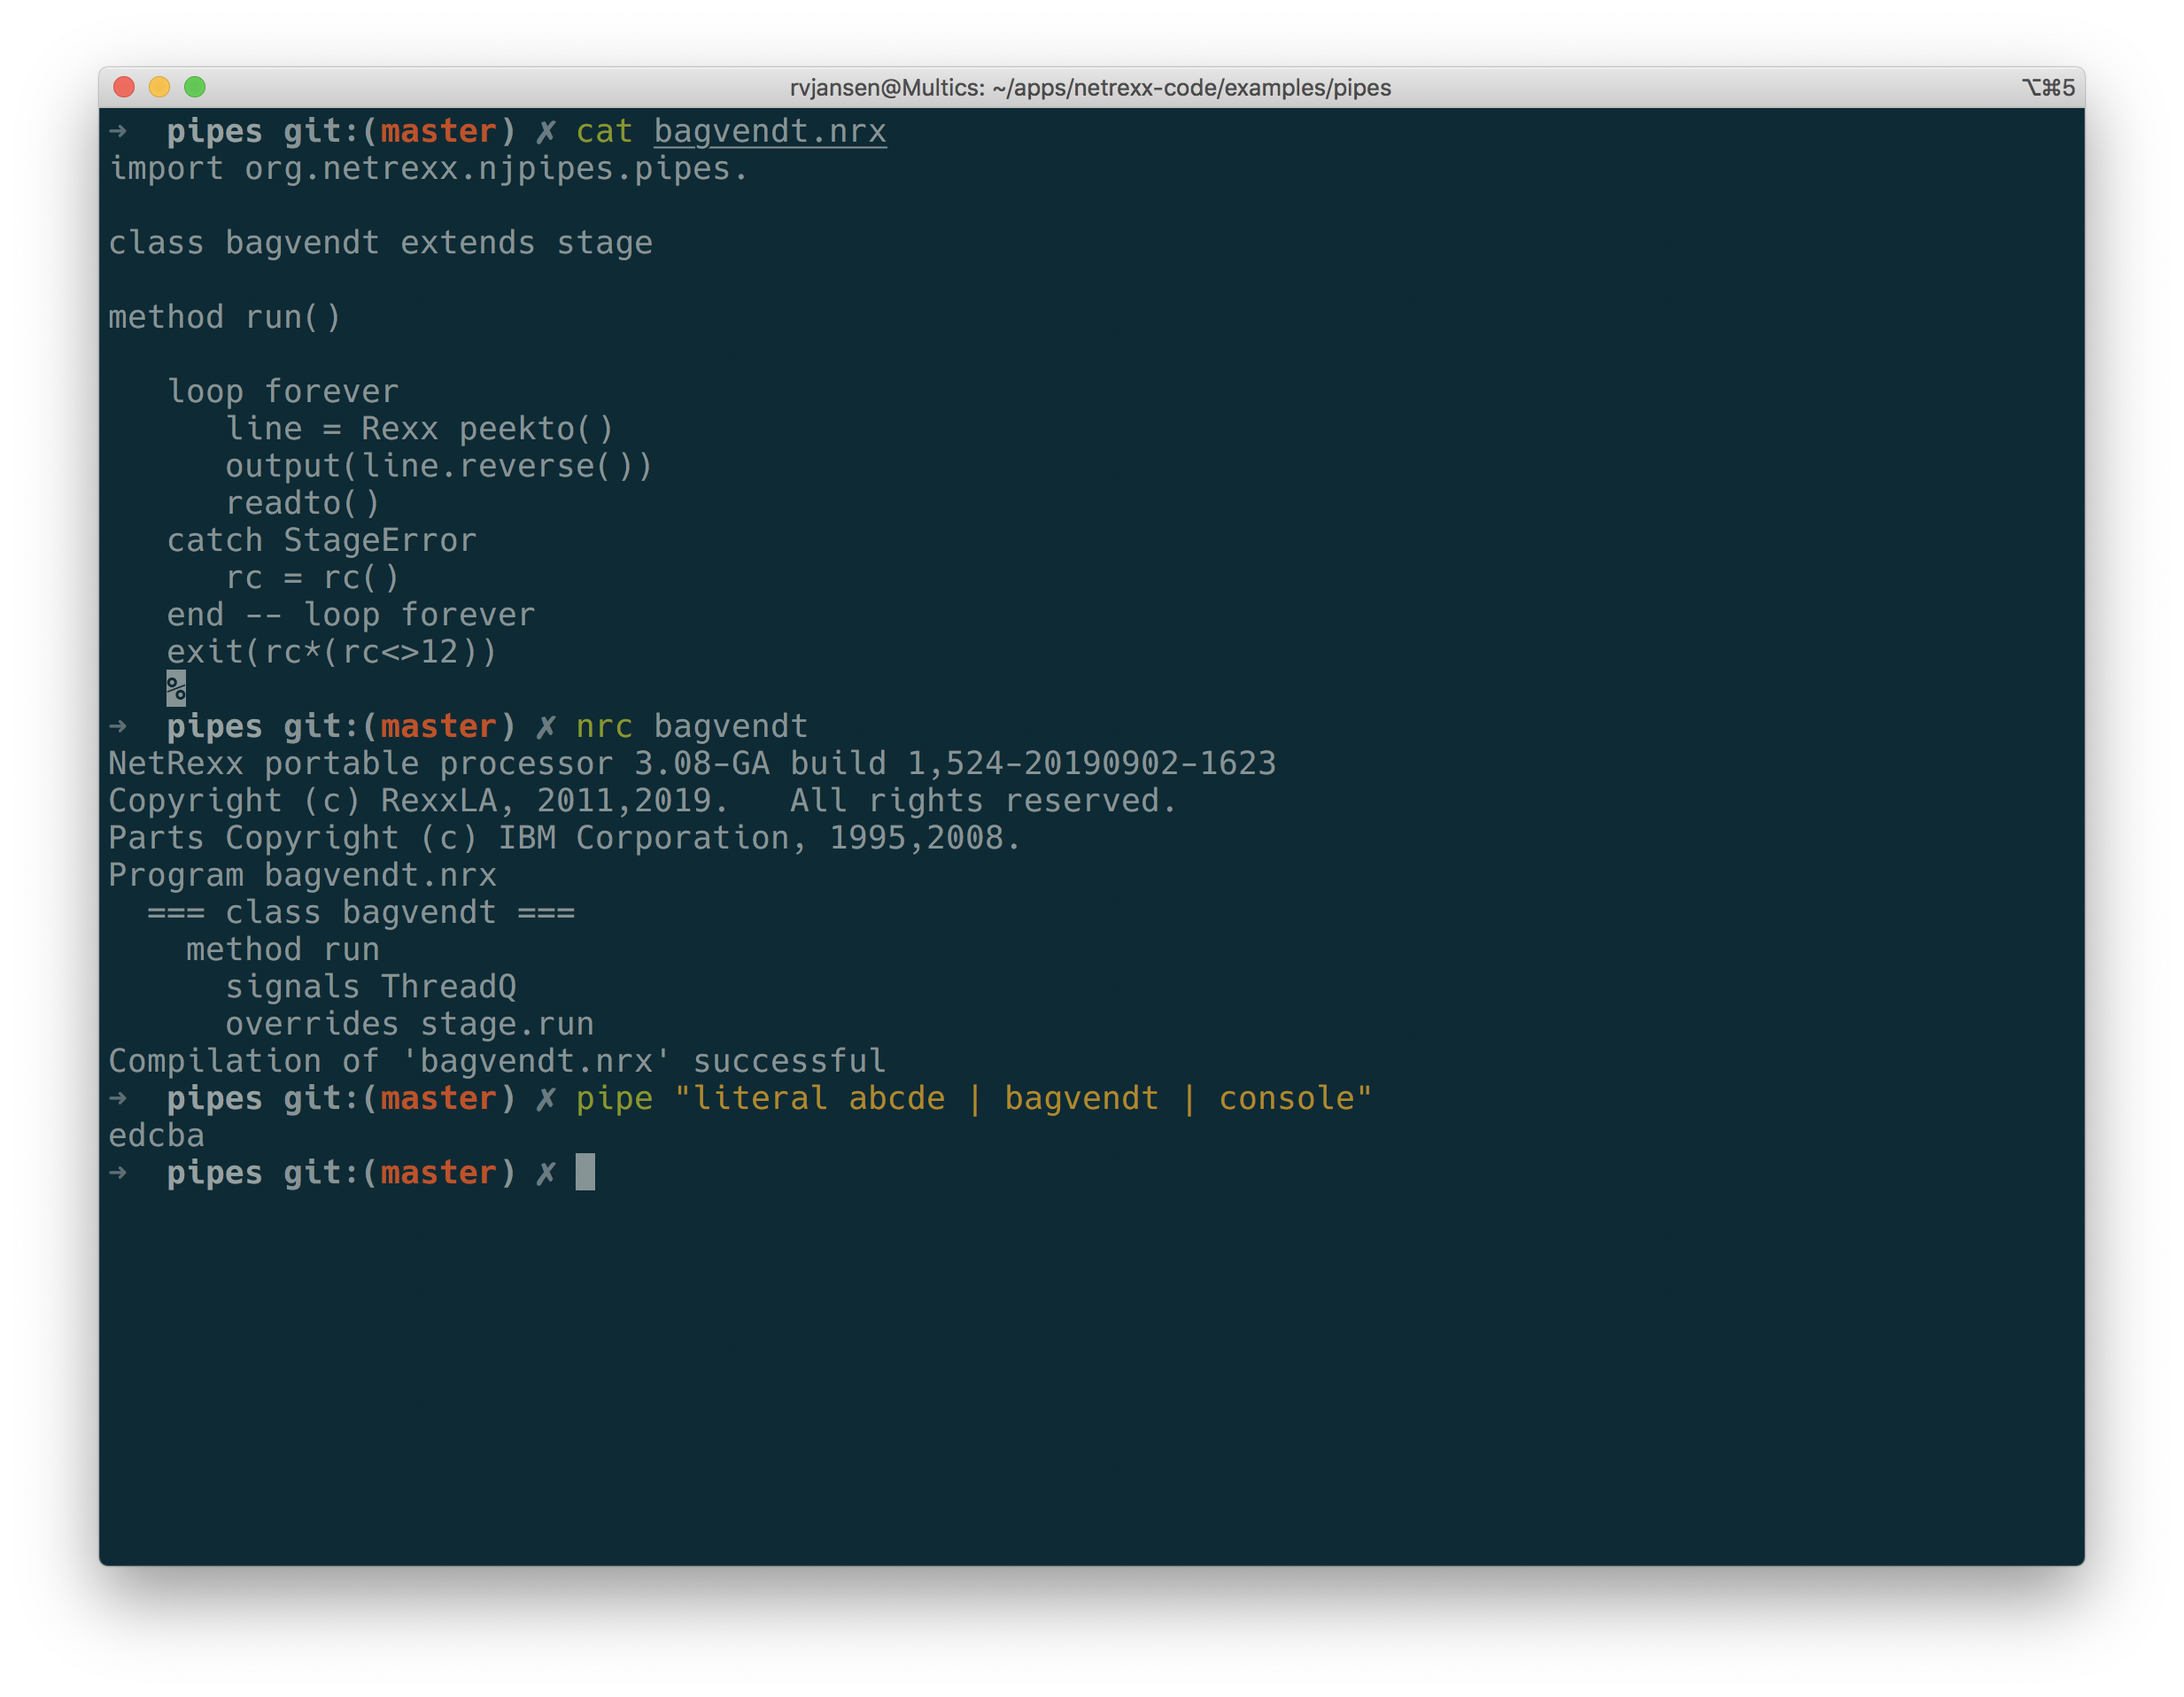
\includegraphics[width=0.75\textwidth]{images/nrbagvendt.png}
  \caption{bagvendt.nrx under \nr{}}
  \label{fig:nrbagvendt}
\end{figure}

\chapter{More advanced Pipelines}
Admittedly, the examples in the previous chapters could have been done
with Unix pipes or at least with incorporation of stream utilities
like awk or sed.


To get a good idea of what can be done with Pipelines for \nr{}, look at the tasktest
pipe in the examples directory.  It \footnote{using code from Melinda Varians
'Cramming for the Journeyman Plumber Exam' paper} implements the
shell of a  multitasking server - using about eight stages.  The file
examples/tcptask.njp contains an example of this technique being used.
\begin{lstlisting}
--tasktest.njp

pipe (tasktest stall 2000 -gen)

   literal 0 1 2 3 4 5 6 7 8 9 A B C D E F G H I J K L M N O P Q R S T |
   dup 2 |
   split |                   -- supply work for task stage

   ptimer |
a: deal secondary ?          -- send work to task stage requesting work
b: faninany |
   elastic |                 -- buffer requests to so no deadlocks
   ptimer |

 a: |
   copy |                    -- buffer work so no deadlocks
   task 1 |                  -- worker task 1
 b: ?

 a: |
   copy |
   task 2 |                  -- worker tast 2...
 b: ?

 a: |
   copy |
   task 3 |
 b:
\end{lstlisting}

Before discussing this example in-depth, we need to go into some more
basic concepts.

\chapter{Device Drivers}
\label{ch:devicedrivers}
Pipelines for \nr{} contains the following device drivers:

\begin{tabularx}{\textwidth}{>{\bfseries}lX}
\toprule
\texttt{<}&read from a fle
\\\midrule
\texttt{>}&write to a file (which is overwritten if it exists)
\\\midrule
\texttt{>>}&append to a file (which is created if it does not exist)
\\\midrule
diskr&read from a fle
\\\midrule
diskw&write to a file (which is overwritten if it exists)
\\\midrule
diska&append to a file (which is created if it does not exist)
\\\midrule
diskslow&read, create or append to a file
\\\midrule
array&manipulate arrays
\\\midrule
arraya&manipulate arrays
\\\midrule
arrayr&manipulate arrays
\\\midrule
stem&manipulate stems
\\\midrule
stema&manipulate stems
\\\midrule
stemr&manipulate stems
\\\midrule
vector&manipulate vectors
\\\midrule
vectora&manipulate vectors
\\\midrule
vectorr&manipulate vectors
\\\midrule
var&read or set a variable in a \nr{} program
\\\midrule
zip&compress a set of files (0 or more) into a zip archive
\\\midrule
unzip&decompress a set of files (0 or more) from a zip archive
\\\midrule
listzip&list a zip file directory
\\\midrule
console& read from, or write to a terminal (window)
\\\midrule
hole&destroy data
\\\midrule
delay&suspend stream
\\\midrule
literal&write the argument string
\\\midrule
strliteral&write the argument string
\\\midrule
sqlselect&select from any jdbc source
\\\midrule
xrange&write a character range
\\\bottomrule
\end{tabularx}


\chapter{Record Selection}
Various stages can select records and work on data in the
pipeline. These are stages called select, sort, specs, locate,
etcetera. For a complete description we refer to the IBM Pipelines
documentation. 

These are the main selection stages supported in Pipelines for \nr{}:

\begin{tabularx}{\textwidth}{>{\bfseries}lX}
\toprule
between&selects records between labels
\\\midrule
drop&discard records from the beginning or the end of a file
\\\midrule
find&select lines
\\\midrule
strfind&select lines
\\\midrule
frlabel&select records from the first one with leading string
\\\midrule
strfrlabel&select records from the first one with leading string
\\\midrule
inside&select records between labels
\\\midrule
locate&select records between labels
\\\midrule
nfind&select lines using xedit nfind logic
\\\midrule
strnfind&select lines using xedit nfind logic
\\\midrule
nlocate&select lines without a string
\\\midrule
notinside&select records not between labels
\\\midrule
outside&select records not between labels
\\\midrule
pick&select records that satisfy a relation
\\\midrule
take&select records from the beginning or the end of a file
\\\midrule
tolabel&select records to the first one with leading string
\\\midrule
strtolabel&select records to the first one with leading string
\\\midrule
unique&discard or retain duplicate lines
\\\bottomrule
\end{tabularx}

\chapter{Filters}
\begin{tabularx}{\textwidth}{>{\bfseries}lX}
\toprule
buffer&buffer records
\\\midrule
chop&truncate the record
\\\midrule
join&join records
\\\midrule
pad&expand short records
\\\midrule
split&split records relative to a target
\\\midrule
change&substitute contents of records
\\\midrule
specs&rearrange contents of records
\\\midrule
xlate&transliterate contents of records
\\\midrule
copy&copy records
\\\midrule
count&count lines, words and bytes
\\\midrule
dup&duplicate the object
\\\midrule
reverse&reverse contents of records
\\\midrule
timestamp&prefix date and time to records
\\\midrule
append&put output from device driver after data on the primary input
\\\midrule
casei&run selection stage in a case-insensitive manner
\\\midrule
not&run stages with output streams inverted
\\\midrule
prefix&Blocks its primary input and excutes stage supplied as an argument
\\\midrule
zone&run selection stage on subset of input record
\\\midrule
elastic&buffer sufficient records to prevent stall
\\\midrule
fanin&concatenate streams
\\\midrule
faninany&copy records from whichever input stream has one
\\\midrule
gate&pass records until stopped
\\\midrule
juxtapose&preface record with marker
\\\midrule
overlay&overlay data from input streams
\\\midrule
command&issue a command and write response to pipeline
\\\bottomrule
\end{tabularx}


\chapter{Other Stages}
\begin{tabularx}{\textwidth}{>{\bfseries}lX}
\toprule
query&check version and level of Pipelines for \nr{}
\\\midrule
\doublehyphenunquoted{}&insert comments into a pipeline
\\\midrule
comment&insert comments into a pipeline
\\\bottomrule
\end{tabularx}


 % \chapter{\nr{} Pipelines Implementation}
% \nr{} Pipelines enables us to follow the usage model of CMS Pipelines
% closely; in fact, the documentation for the mainframe product can be
% used for most stages.

% \section{Installation and verification}
% To run \nr{} Pipelines a running \nr{} installation is needed.  To write your own pipes or stages you need compilers for both Java and \nr{}. 
% The core classes for pipes and stages are in the archive \nr{}F.jar.  This file may
% be used on the -cp option or added to your CLASSPATH, as indicated in
% the \emph{\nr{} Quickstart Guide}.

% To test the installation, we can run a pipeline from the command line.
% Running a pipeline from the command line
%  To run a pipeline from the commandline, type:
% \begin{lstlisting}
% pipe 'gen 100 | dup 999 | count words | console'
% \end{lstlisting}

% Remember to use double quotes on Windows shells. When the \texttt{pipe}
% alias or command script is not on your path, you can also use:

% \begin{lstlisting}
% java org.netrexx.njpipes.pipes.runner 'gen 100 | dup 999 | count words | console'
% \end{lstlisting}

% In both cases the answer should be 100000 - you have generated one
% hundred thousand lines, but fortunately you did not print them, but
% only counted them. To see them all, you can insert a | console | stage
% in between the dup and the count stage.

\chapter{Multi-Stream Pipelines}
One of the defining differences with Unix pipes is the possibility to
define multi-stream pipelines. The selection stages from the previous
chapter all have \emph{secondary streams}. What the selection
parameters have discarded, \emph{seem to have discarded}, is in
reality not gone. In fact, Pipelines for \nr{} throws very little away during
execution.

The way to use the not-selected part of the data through
these secondary streams is explained in this chapter; it is this
capacity that constitutes the freedom to work with many different
streams in one pipeline; where Unix pipes are limited to not very much
more than stdin, stdout, stderr -- Pipelines for \nr{} enables the user
to define as many streams as necessary to accomplish the task at hand
in an efficient manner.

Let us look at a simple selection like the following:

\begin{lstlisting}
 pipe literal foo bar baz frob frobnitz frobbotzim | split | locate /oo/ |
 console
\end{lstlisting}
\begin{verbatim}
foo
\end{verbatim}
The string that makes it through the selection that is done by the
\emph{locate} is 'foo' - it is the only one that is captured by the
/oo/ filter.

The rest of the words is not gone, however, and we can use these in
further processing by using the secondary stream that \emph{locate}
provides.

To prepare for this, we give the secondary stream a name by providing
a label for it, we call it, in absence of any creativity,
\emph{rest}\footnote{often, you will see it being called 'a:'}. Also, we send the selected output, \texttt{foo} into a
\emph{hole} stage, where it disappears.
\begin{lstlisting}
 pipe literal foo bar baz frob frobnitz frobbotzim | split | rest: locate /oo/ |
 hole
\end{lstlisting}
As predicted, there is no output. To get to the rest of the words,
unselected by \emph{locate}, we connect the secondare output stream to
a new pipe, using the '?' (the default pipe-end character) like this:
\begin{lstlisting}
 pipe literal foo bar baz frob frobnitz frobbotzim | split | rest: locate /oo/ |
 hole ? rest: | console
\end{lstlisting}
The output is now:
\begin{verbatim}
bar
baz
frob
frobnitz
frobbotzim
\end{verbatim}

Instead of sending the original output into a black \emph{hole}, we
could have also gone further with it, and, for example, reverse it:
\begin{lstlisting}
 pipe literal foo bar baz frob frobnitz frobbotzim | split | rest: locate /oo/ |
 reverse | console  ? rest: | console
\end{lstlisting}
The output is now:
\begin{verbatim}
oof
bar
baz
frob
frobnitz
frobbotzim
\end{verbatim}
Likewise, we can specify more filter stages in the second, attached
pipeline, and bifurcate the pipeline even further.

\begin{lstlisting}
 pipe literal foo bar baz frob frobnitz frobbotzim | split | rest: locate /oo/ |
 reverse | console  ? rest: | locate /botzim/ | console
\end{lstlisting}
The output is now:
\begin{verbatim}
oof
frobbotzim
\end{verbatim}




It is good to define and implement secondary streams when you write
your own stages.


\chapter{Pipeline Stalls}
With multistream pipelines a new problem sometimes rears its head - a \emph{Pipeline stall}, also called \emph{deadlock}. This happens when stages
wait for input that cannot be delivered, in a way that ensures that it
cannot be delivered.

Pipes for \nr{} detects deadlocks and outputs information to allow you to fix the problem.  Consider the following session:
\begin{lstlisting}
pipe literal test | a: fanin | console | a:
\end{lstlisting}

\begin{figure}[h]
  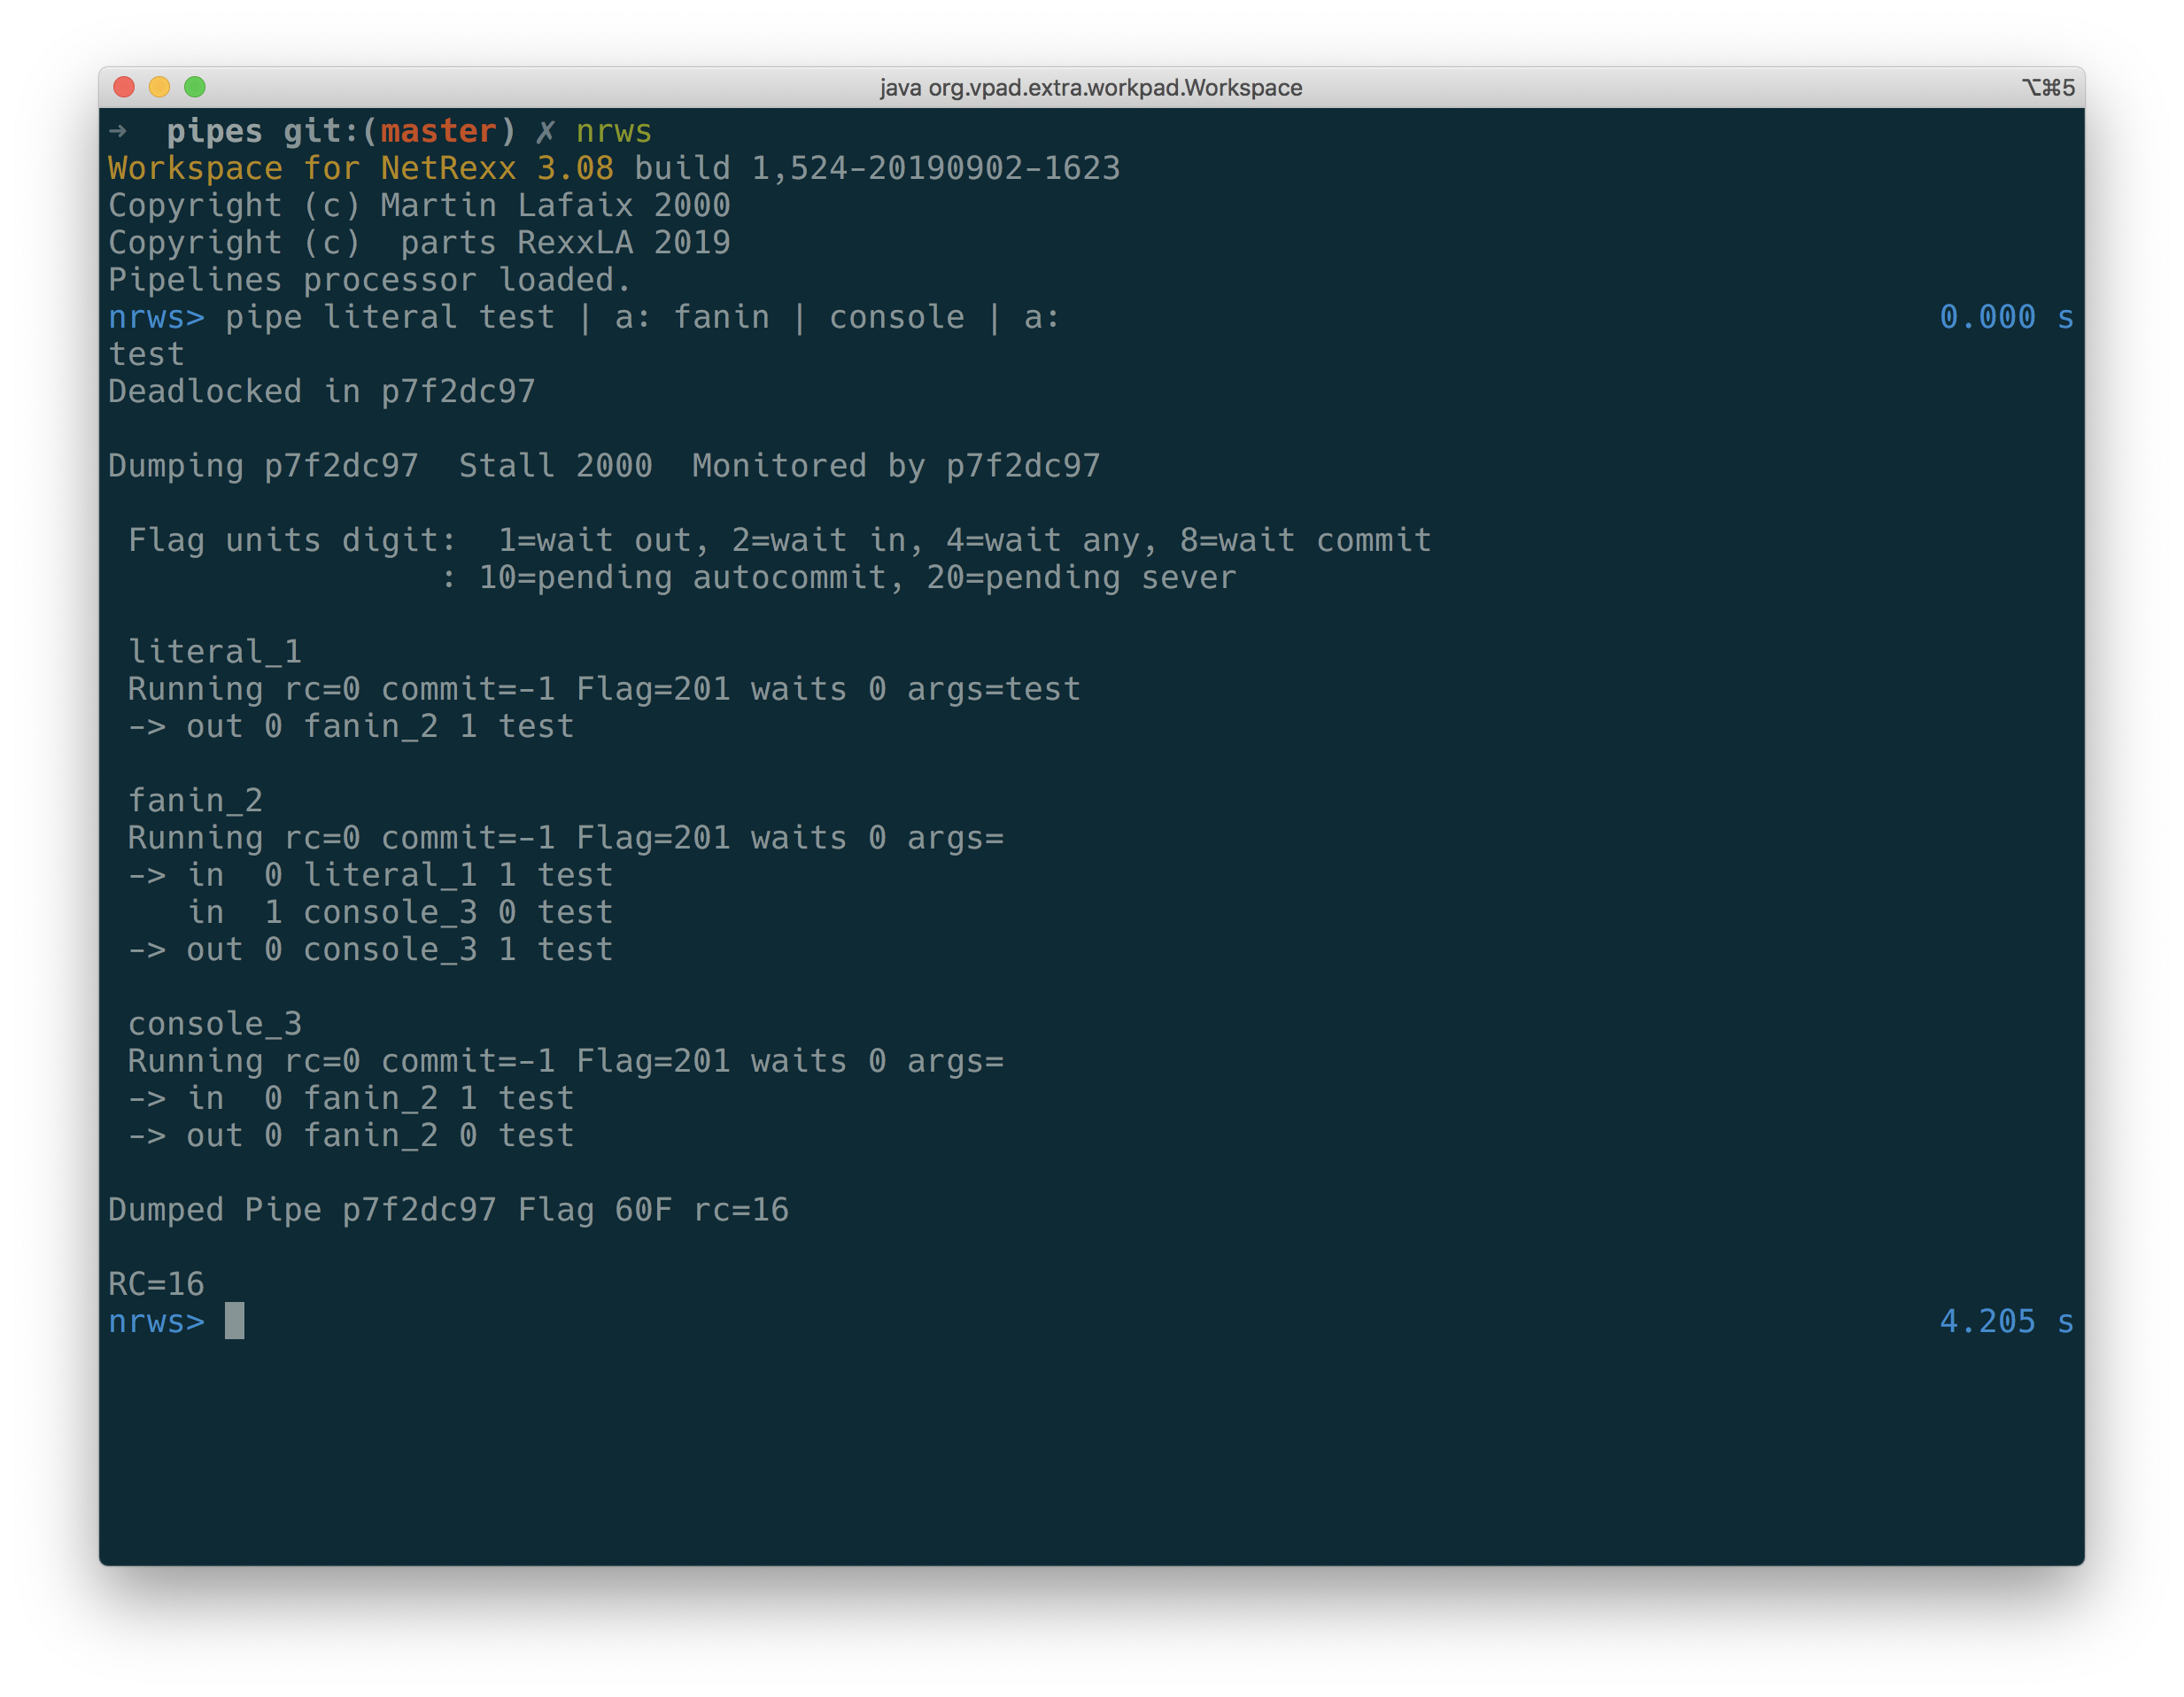
\includegraphics[width=0.75\textwidth]{images/deadlock.png}
  \caption{Deadlock detection}
  \label{fig:tcpcompile}
\end{figure}

We can see that there are three stages in the Running state.  None
have any return codes set.  The Flags tell us that all the stages are
waiting for an output to complete.

The '->' show which stream is
selected.  From this we can see console\_3 is trying to output to
fanin\_2. Unfortunately fanin\_2 is waiting for output on stream 0 to
complete, it cannot read the data waiting on in stream 1.  Hence the
stall.

The strings after \emph{Dumping} and \emph{Monitored by} are the
autogenerated class names. When you name your pipelines with
precompiled pipes yourself, the names you have given them will be displayed here.

When a stream has data being output, there is a boolean flag following the name of the stage the stream is connected to. This tracks the peek state of the object.  For an output stream, true means the following stage has peeked at the value. With input streams, the current stage has seen the value when its true.

When a stage is multithreaded, like elastic, you can get flags of 3 or 5. This means that threads are waiting on output and read, or output and any. When using multithreaded stages, only one thread should use output unless it is serialized using protected or syncronized blocks.

When a stage has a pending sever or autocommit, flag bits are set too.




% In z/VM CMS, it is quite common to use a pipe in a Rexx exec. Conversely,
% often a stage is written in Rexx. In Pipes for
% \nr{} it is also easy to write your own stages. Both scenarios are
% shown in this chapter.

% Writing your own pipes or stage is simple.  Take a look at the source
% of the supplied stages in the stages directory.  Input can be supplied
% on the commandline, in which case the arguments to the \nr{} program
% are used; when the input comes \emph{through the pipleline}, the
% methods \begin{alltt}peekto(), readto()\end{alltt}
% and \begin{alltt}output()\end{alltt} methods. Here are some more
% examples.
% \begin{lstlisting}
% class length extends stage final
 
%   method run()
%     do
%       loop forever
%     line = rexx peekto()
%     l = line.length
%     output(l l.d2x line)
%     readto()
%       end
%     catch StageError
%       rc = rc()
%     end
%     exit(rc*(rc<>12))
%   \end{lstlisting}
  
\chapter{How to use a pipe in a \nr{} program}

This shows how to use a pipe in a \nr{} program:

\begin{lstlisting}
 class testpipe

    method testpipe(avar=Rexx)

       F = Rexx 'abase'
       T = Rexx 1

       F[0]=5
       F[1]=222
       F[2]=3333
       F[3]=1111
       F[4]=55
       F[5]=444

       pipe (apipe stall 1000 )
         stem F | sort | prefix literal {avar} | console | stem T

       loop i=1 to T[0]
          say 'T['i']='T[i]
       end

    method main(a=String[]) static

       testpipe(Rexx(a))
\end{lstlisting}
 A couple of things can be seen in this example.  First that it is
 simple to pass \nr{} variables to pipes using \emph{stem}.  Also look
 at the phrase \texttt{ \{avar\}}. It passes the \nr{} variable's value to the stage at runtime.  In CMS the pipe would be quoted and you would unquote sections to get a similiar effect.

 Another thing to note is that the pipe extraction program is fairly smart. It detects when pipes takes several lines.  As long as there are stages, or the current line ends with a stagesep or stageend character, or the next line starts with a stagesep or stageend character.  It gets added to the pipe.

 The arg(), arg(rexx) or arg(null) methods get the arguments passed to
 a stage or pipe.  To get the complete rexx string of an argument use
 arg(). To get the nth word of a rexx argument use arg(n).  When using
 pipes in netrexx code you can use arg('name') to get the named
 argument. If the class of the argument is not rexx use arg(null) to
 get the object.
 
In .njp files you can use {avar} phrase actually just shorthand for  arg('avar').
The following example shows what has to be done in a stage to access the rexx variables passed by VAR, STEM and OVER.  The real  over stage is a bit more complete.
\begin{lstlisting}
    -- over.nrx
 class over extends stage final

    method run() public
        a = getRexx(arg())
      loop i over a
         output(a[i])
      catch StageError
         rc = rc()
      end
    
   exit(rc*(rc<>12))
\end{lstlisting}
 The getRexx method is passed the name of a string by the pipe.  In the previous example it would be passed A and would return an Object pointer to A in testpipe. If you wish to replace a stream this can be done using connectors.  For example look at the following fragment:
\begin{verbatim}
    -- examples\calltest.njp
    pipe (callt1) literal test | calltest {} | console
\end{verbatim}
\begin{lstlisting}
    import org.netrexx.njpipes.pipes.

    class calltest extends stage final

    method run() public

       do
          a = arg()

          callpipe (cp1) gen {a} | *out0:

          loop forever
             line = peekto()
             output(line)
             readto()
          end

       catch StageError
          rc = rc()
       end

    exit(rc*(rc<>12))
\end{lstlisting}
Running the callt1 pipe with an argument of 10 would pass the 10 to calltest via {} and arg().  Then cp1's gen stage would be passed 'a' which is set to 10.  Since gen generate numbers in sequence, the console stage of callt1 would get the numbers from 1 to 10.  Now cp1 ends and calltest's output stream is restored and calltest unblocks and reads the the literal's data 'test' and passes it to console.

The use of {} only works when compiling from .njp files.  It will not work from the command line.
The njpipes compiler recognizes connectors as labels with the following forms:
\begin{verbatim}
    *in:
   *inN:
   *out:
   *outN
\end{verbatim}

When N is a whole number, the connector connects input or output stream N of the stage with the connector.
When the label *in or *out, the connector connects the stages's current input or output stream with the connector.  This is used instead of *: due to the way the compiler/preprocessor works.
If you do not want the stage to wait for the called pipe to complete you can use addpipe.  Here is an example.
\begin{lstlisting}
    -- similar to examples\addtest.njp

    a  = 100
    b  = 'some text for literal'

    addpipe (linktest) literal {b} | dup {a} | *in0:

    loop forever
       line = Rexx readto()
    catch StageError
    end
\end{lstlisting}
    readto() will get 'some text for literal' one hundred times.

A quick aside.  When writing stages remember that njPipes moves objects through pipes.  Use 'value = peekto()' instead of 'value = rexx peekto()' when ever possible.  Some of the supplied stages pass objects with classes other than rexx and forcing rexx will cause classCastExceptions. If a stage needs a rexx object try using the rexx stage modifier to attempt to convert the object.  Feel free to expand this stage, but please send me the updated version.

Serious stage writers will probably want to take a good look at the
methods defined in the \nr{} source package \texttt{org.netrexx.process.njpipes.stages}.  There you will find various methods for parsing ranges.  You will also find the stub for the stageExit compiler exit.  It can be used to produce 'on the fly' code at compile time.  You can also use it to change the topology of the unprocessed part of the pipe.  The major use is to allow implementations of stages like prefix, append or zone.  Its also used to produce better performing stages, for an example see specs.
The compiler also queries the rexxArg() and stageArg() methods.  If your stage expects objects of class Rexx as arguments rexxArg() should return the number of variables expected.  If your stage expects a stage for an argument, stageArg() should return the word position of the stage.

\chapter{Giving commands to the operating system}

The \texttt{command} stage is used to issue commands to the operating
system and trap the output to the pipeline. \texttt{command} can
receive its input as parameters, or through the pipeline. So
\begin{lstlisting}
  pipe literal ls | command | sort | console
\end{lstlisting}
is equivalent to:
\begin{lstlisting}
  pipe command ls | sort | console
\end{lstlisting}


\section{Built-ins}
Some commands, like \texttt{dir} in Windows, do not have a separate
executable file; there is no \texttt{dir.exe}. This can be solved by
having the command processor, \texttt{cmd.exe} start its built-in
command. The pipeline would be, for example:
\begin{lstlisting}
  pipe literal cmd /c dir | command | sort | console
\end{lstlisting}
\chapter{TCP/IP Networking using Pipes for \nr{}}
As the built-in stages all work on data that is dispatched through the
pipeline, irrespective of which device driver is used, it is also
convenient to do network programming using a set of pipelines.

The \emph{tcplisten} stage can be used as a network device driver, as
in CMS, but limited to specification of the port and a timeout value. Below an example of how to implement a sample TCP/IP
client/server application.
\begin{lstlisting}
-- one shot tcpip server

pipe (tcpserv stall 60000 debug 0 )
   tcplisten 1958 timeout 15000 | tcpexample

-- one shot tcpip requestor

pipe (tcpreq stall 60000 debug 0 )
   random {} |
   specs *-* 1 ,\n, next |
   tcpclient deblock c localhost 1958 timeout 10000 linger 500 oneresponse |
   rexx to console

-- a single tasking server

options binary
import org.netrexx.njpipes.pipes.
class tcpexample extends stage

method run() public

   loop forever

      peekto()

      callpipe (tcplog stall 15000 debug 0)
         *in0: |
         take first 1 |
         console |
      f: fanin |
         tcpdata timeout 10000 deblock C oneresponse |
         elastic |
         insert /\n/ after |
      f:

   catch StageError
      rc = rc()
   end

exit(rc*(rc<>12))
\end{lstlisting}
This example needs to be compiled with the pipes compiler, see
\emph{TCP/IP Client/Server compile}, which yields the classes tcpserv
and tcpreq, for the server and the requester component. 
\begin{figure}[h]
  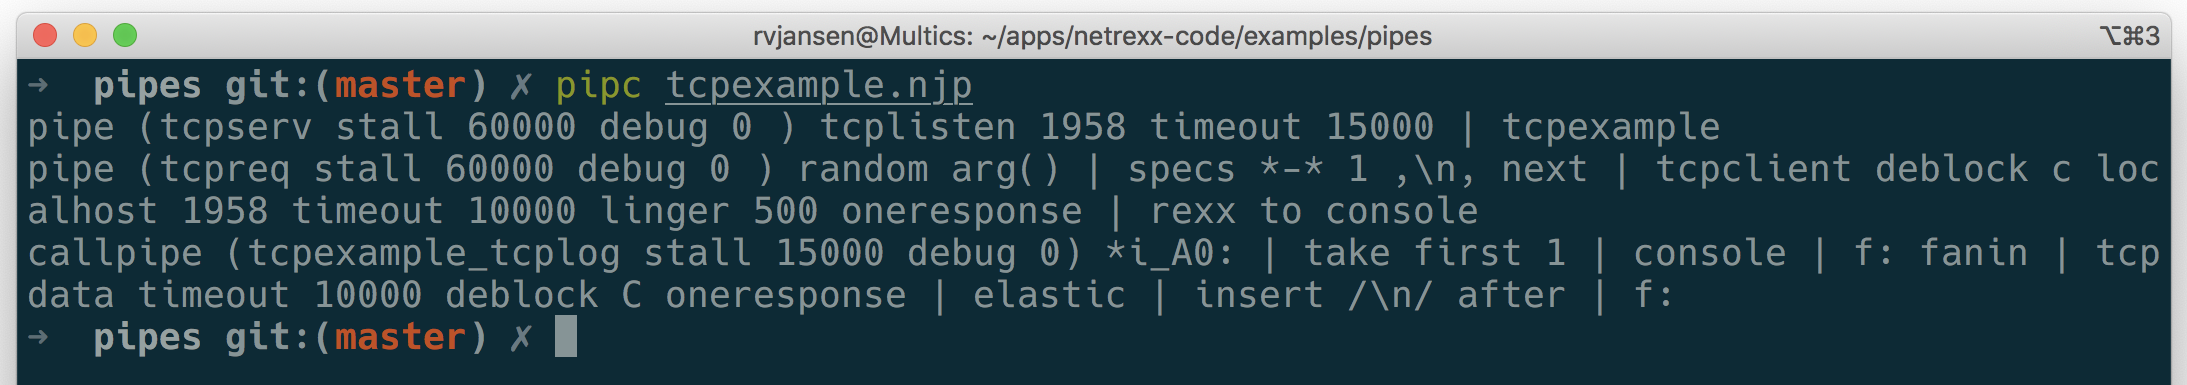
\includegraphics[width=0.75\textwidth]{images/tcpcompile.png}
  \caption{TCP/IP Client/Server compile}
  \label{fig:tcpcompile}
\end{figure}

Now we can start the generated pipelines each in their own shell
window. As can be seen in \emph{TCP/IP server}, the class keeps
waiting on connections on port 1958 - which is arbitrary, but
specified in the pipeline source.

\begin{figure}[h]
  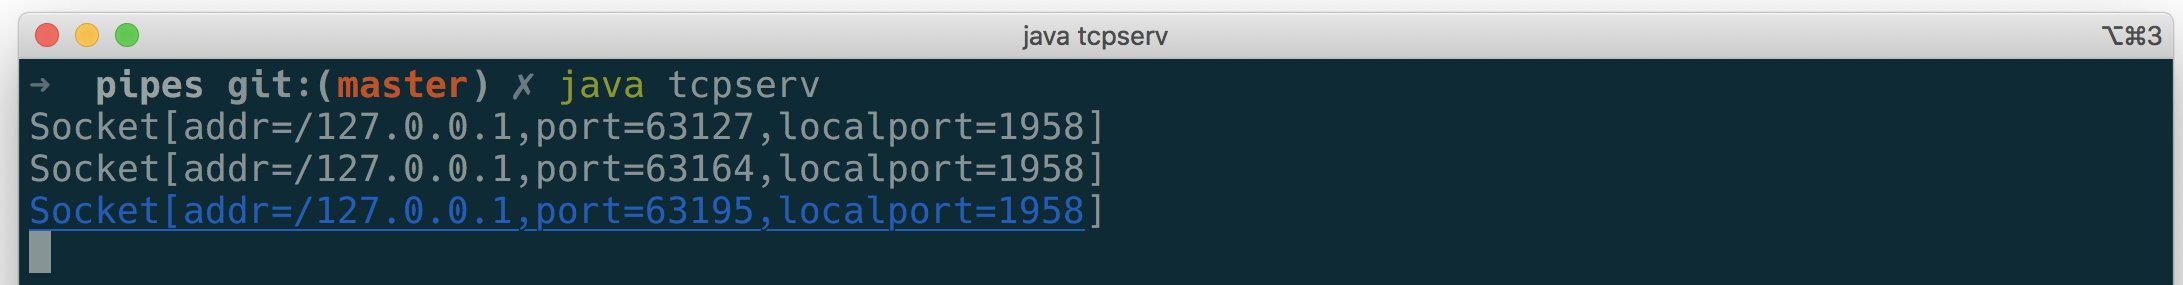
\includegraphics[width=0.75\textwidth]{images/tcpserv.png}
  \caption{TCP/IP server}
  \label{fig:tcpcompile}
\end{figure}

In another window, we can start the \emph{TCP/IP requestor}, which
when given port 1958 as argument, connects to the server, and displays
a series of random numbers that is sent to it.

\begin{figure}[h]
  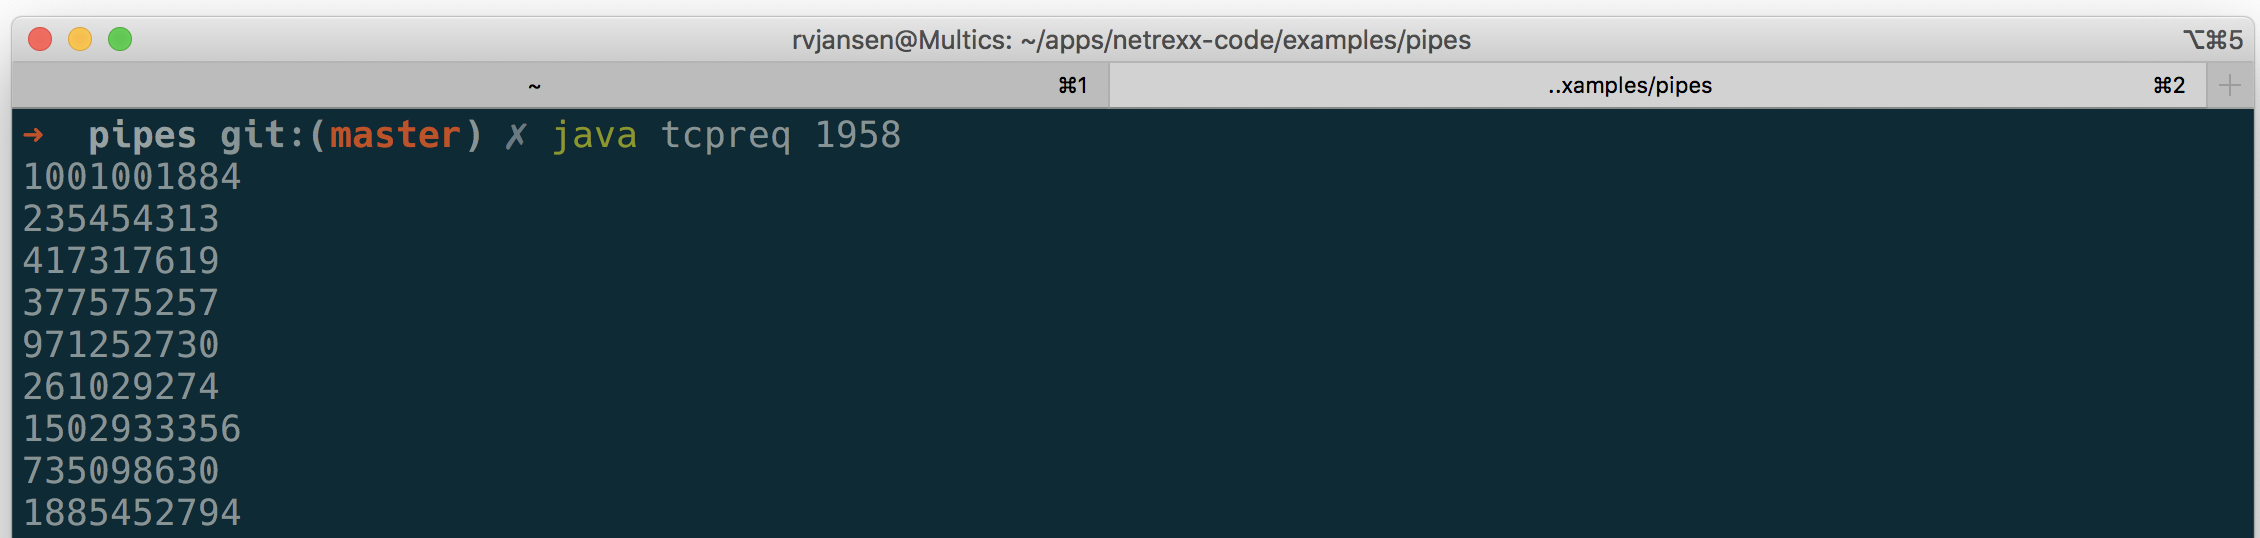
\includegraphics[width=0.75\textwidth]{images/tcpreq.png}
  \caption{TCP/IP requestor}
  \label{fig:tcpcompile}
\end{figure}

Note that the stage \emph{tcpexample} from the \emph{tcpserver}
pipeline is a custom stage that is written in this tcpexample.njp
file.

\chapter{Selecting from databases with Pipelines for \nr{}}

Using the built-in \emph{sqlselect} stage you can select data, using
SQL, from any jdbc source available.

An \texttt{sqlselect.properties} file is needed to define the jdbc parameters
like the driver to use, the url of the data source and other
arguments, like a password and tracing options, if needed.

The file looks like this:
\begin{verbatim}
jdbcdriver=org.sqlite.JDBC
url=jdbc:sqlite:flightroute-iata.sqb
\end{verbatim}

This is all that is needed for an sqlite database containing flight
data. A simple select * can then be done with the following pipeline:

\begin{lstlisting}
pipe literal * from FlightRoute where flight = 'KLM765' | sqlselect | console
\end{lstlisting}

This yields the following output:
\begin{verbatim}
FLIGHT--ROUTE--UPDATETIME--
KLM765  AUA-BON-AMS  1494132448
\end{verbatim}

\begin{shaded}
Note that from the command line, the quotes around the pipe
specification and the literal string in the SQL statement should be
opposite, while when the pipeline is issued from the Workspace for
\nr{}, the pipeline does not have to be quoted, but the sql string
needs double quotes instead of the - for SQL statements- normal single quotes.
\end{shaded}
\chapter{The Pipes Runner}
The pipes compiler is used in both precompiled and directly executed
pipelines. When you directly execute a pipeline from the commandline
or from the \emph{nrws} \nr{} workspace, the process is optimized to not persist
generated \nr{}, Java and Class files to disk before execution; the
whole process runs from memory. The Pipes Runner uses the Pipes
Compiler for this purpose, and as such misses the options for
persistence\footnote{But specifying them will not generate an error}.

The \emph{pipe} command alias start the Pipes Runner, which is a
command processor that can execute a pipe from the command line in an
OS shell, the OS being Windows, Linux or macOS\footnote{this is a
  non-exhaustive list of operating systems}.

A pipe can be run with options prepended within parentheses, like this:
\begin{lstlisting}
pipe '(test1 sep ! stall 2000 debug 63) literal abcde ! console'
\end{lstlisting}

The following options are
available:

\begin{tabularx}{\textwidth}{>{\bfseries}lX}
\toprule
pipename&Specify the name of the generated class file. This
can be useful for debugging purposes but is not mandatory when running
a pipe. An unnamed pipe receives a generated unique name. This option
needs to go first.
\\\midrule
sep&The default stage separator is the |
(pipe) character; this can be overridden with the sep option; a pipe
called test1 which uses an exclamation mark as separator character,
needs the options (test1 sep !).
\\\midrule
debug&The debug option specifies a bitmask for
debugging the execution of a pipe; (debug 63), for
example, generates a rather complete debugging trail).
\\\midrule
end&The default pipe end character is the ' ?'
  (question mark), which can be overridden here. Note that the
  backslash, which is an obvious pipe end character for the z/VM 3270
  interface, is not a good choice for Windows and Unix shells.
  \\\midrule
stall& The duration in number of seconds of a pipe stall (or deadlock)
detection cycle.
\\\bottomrule
\end{tabularx}


\chapter{The Pipes Compiler}
The purpose of precompiling a pipeline specification is to produce a
.class file for the JVM that can be run independently and on different
machines; only the JVM and the NetRexxC.jar or the NetRexxF.jar are
required to run a precompiled pipe. A set of precompiled pipes can be
shipped as an application.

When precompiling pipes, there are options to save and view the
generated \nr{}, Java and JVM Class files. A precompiled pipe has
the advantage that it can be executed over and over in an application,
without the need to compile it every time; the performance savings are
accumulative in this scenario.

The following options can be used on the \emph{pipc} command, in
addition to the ones specified in the previous chapter for the Pipes Runner:

\begin{tabularx}{\textwidth}{>{\bfseries}lX}
\toprule
-gen&Generate the \nr{} source file. The pipeline needs a name.
\\\midrule
-keep&Keep the Java source which is generated from the \nr{} source.
\\\bottomrule
\end{tabularx}

Example:
\begin{lstlisting}
pipe (testpipe -gen -keep)
\end{lstlisting}
This will generate the \nr{} source as well as keep the java source.



\chapter{Built-in Stages}
This section describes the set of built-in stages, i.e. the ones that
are delivered with the downloadable open source package. These stages
are directly executable from the NetRexxC.jar file or the NetRexxF.jar
file (the latter contains a Java compiler for use on JRE-only
systems); also, the source of these stages is delivered in the \nr{}
source repository. This repository can be checked out at
\begin{verbatim}
git clone https://git.code.sf.net/p/netrexx/code netrexx-code
\end{verbatim}
The source of the stages is in directory
\begin{verbatim}
netrexx-code/src/org/netrexx/njpipes/stages
\end{verbatim}

% \chapter{Stages}
\section{abbrev}
\index{abbrev}
\begin{shaded}
\begin{rail}
  abbrev : 'abbrev'( word?|number?)'ANYCASE'?
  ;
\end{rail}
\end{shaded}

\textbf{Type:} Selection Stage

\textbf{Syntax Description:} A word, a number and a keyword are
optional.

The word specifies the characters to compare against the beginning of
input records. The default is a null word. The number specifies the
minimum count of characters that must be present to select the
record. The default is zero, which means that any abbreviation down to
a null record or a leading blank will be selected. Specify ANYCASE to
make the comparison case insensitive. 

\textbf{Operation:}  \emph{abbrev} compares the leading columns of
each record against the specified word until a blank or the end of the
record is met. The record is passed to the primary output stream if a
minimum abbreviation of the specified word is present. Otherwise, the
record is discarded (or passed to the secondary output stream if the
secondary output stream is connected).

\textbf{Example}:
\lstinputlisting[label=abbrev1,caption=abbrev example]{abbrevsample.njp} 
\bash[stdout]
pipc abbrevsample
\END
\bash[stdout]
java abbrev1
\END

\section{append}
\index{append}
\begin{shaded}
\begin{rail}
  append : 'append' string
  ;
\end{rail}
\end{shaded}

\textbf{Type:} Control

\textbf{Syntax Description:} The argument string is normally a single stage, but any pipeline
specification that can be suffixed by a connector (|*:) is acceptable.

\textbf{Operation:} All records on the primary input stream are copied
to the primary output stream. Then the string is issued as a
subroutine pipeline with CALLPIPE, using the default stage separator
(|), double quotes as the escape character ("), and the backward slash
as the end character. The beginning of the pipeline is
unconnected. The end of the pipeline is connected to append’s primary
output stream. (Do not write an explicit connector.)

\textbf{Example:}

\lstinputlisting[label=append1,caption=append example]{appendsample.njp} 
\bash[stdout]
pipc appendsample
\END
\bash[stdout]
java appendtest
\END



\section{between}
\index{between}
\begin{shaded}
\begin{rail}
  between : 'between' 'ANYcase'? delimitedString ( delimitedString?|number?)
  ;
\end{rail}
\end{shaded}

\textbf{Type:} Selection Stage

\textbf{Syntax Description:}


\textbf{Operation:}  \emph{between}

% \textbf{Example}:
% \lstinputlisting[label=between1,caption=between example]{betweensample.njp} 
% \bash[stdout]
% pipe betweensample
% \END
% \bash[stdout]
% java between1
% \END

\section{buffer}
\index{buffer}
\begin{shaded}
\begin{alltt}
/** buffer


   >>--BUFFER--+-----------------------------+----------------------------><
               +-number--+-----------------+-+
                         +-delimitedString-+

\end{alltt}
\end{shaded}

\section{casei}
\index{casei}
\begin{shaded}
\begin{alltt}
\end{alltt}
\end{shaded}

\section{change}
\index{change}
\begin{shaded}
\begin{alltt}
/** change

  >>--CHANGE--+---------+--+-----------------+---------------------------->
              +-ANYcase-+  +-inputRange------+
                           |    <-------+    |
                           +-(----range-+--)-+

  >--+-+ changeString +-----------------+--+-----------+-----------------><
     +-delimitedString--delimitedString-+  +-numorstar-+

  changeString:
  +--delimiter--string--delimiter--string--delimiter----------------------+

\end{alltt}
\end{shaded}

\section{chop}
\index{chop}
\begin{shaded}
\begin{alltt}
/** chop

                     +-80-----+
   >>--+-CHOP-----+--+--------+-------------------------------------------><
       +-TRUNCate-+  +-number-+



   >>--CHOP--+---------+--+-------------------------+--+-----+------------->
             +-ANYCase-+  |              +-BEFORE-+ |  +-NOT-+
                          +-+---------+--+--------+-+
                            +-snumber-+  +-AFTER--+

   >--+ target +----------------------------------------------------------><

   target:
   +--+-xrange----------------------+--------------------------------------+
      +-+-STRing-+--delimitedString-+
        +-ANYof--+


\end{alltt}
\end{shaded}

\section{command}
\index{command}
\begin{shaded}
\begin{alltt}
\end{alltt}
\end{shaded}

\section{compare}
\index{compare}
\begin{shaded}
\begin{alltt}
/** compare

               +-TRINARY-+  (1)           +-PAD SPACE-+
  >>--COMPARE--+---------+------------+---+-----------+----------------------><
               +-BINARY--+  (2)       |   +-PAD-Xorc--+
               |                      |
               | <-----------------+  |
               +--ANY DString------+--+   (4) (5)
               +--EQUAL DString----+      (4)
               +--LESS DString-----+  (3) (4)
               +--MORE DString-----+  (3) (4)
               +--NOTEQUAL DString-+      (4)

     (1) -1 = Primary is shorter/less, 0 = equal, 1 = Secondary is shorter/less
     (2) 0 = equal, 1 = not equal
     (3) Primary is LESS/shorter (or MORE/longer) than secondary
     (4) DStrings can use any of the following escapes (or the lowercase) for
         the unequal situation:
\begin{verbatim}
                 \C (count) for the record number,
                 \B (byte) for column number
                 \P (primary) for the primary stream record
                 \S (secondary) for the secondary stream record
                 \L (Least) for then stream number that is shortest, -1 if equal
                 \M (Most) for the stream number that is longest, -1 if equal
     (5) Equal or not, this DString precedes any of the others.
\end{verbatim}
\end{alltt}
\end{shaded}

\section{console}
\index{console}
\begin{shaded}
\begin{alltt}
/** console

                                               { CMS Only                 }
                                               {                          }
   >>--+-CONSole--+--+----------------------+- { -+----------------+----- } ----><
       +-TERMinal-+  +-EOF--delimitedString-+  {  +-DIRECT---------+      }
                     +-NOEOF----------------+  {  +-ASYNchronously-+      }
                                               {  +-DARK-----------+      }
\end{alltt}
\end{shaded}

\section{copy}
\index{copy}
\begin{shaded}
\begin{alltt}
/** copy

copy from input stream to output without delaying the stream.   See elastic
for a more generic way to do this.

\end{alltt}
\end{shaded}

\section{count}
\index{count}
\begin{shaded}
\begin{alltt}
/** count


              <--------------+
   >>--COUNT--++-CHARACTErs-++--------------------------------------------><
               +-WORDS------+
               +-LINES------+
               +-MINline----+
               +-MAXline----+

\end{alltt}
\end{shaded}

\section{dam}
\index{dam}
\begin{shaded}
\begin{alltt}
/** dam

Do no pass any objects thru secondary streams until an object apprears
on the primary input stream.  The primary output stream must not be
connected.

\end{alltt}
\end{shaded}

\section{deal}
\index{deal}
\begin{shaded}
\begin{alltt}
/** DEAL


            +-STOP--ALLEOF--------------------+
  >>--DEAL--+---------------------------------+--------------------------><
            +-STOP--+-ALLEOF-+----------------+
            |       +-ANYEOF-+                |
            |       +-number-+                |
            +-SECONDARY--+---------+----------+
            |            +-RELEASE-+          |
            +-KEY--inputRange--+-------+------+
            |                  +-STRIP-+      |
            +-STREAMid--inputRange--+-------+-+
                                    +-STRIP-+

  Since java dispatches the stage threads.  Deal may not see a sever immediatly,
  as the severing thread can get multitasked.  This can make options like 'ANYEOF' 
  work in unexpected ways. 

\end{alltt}
\end{shaded}

\section{deblock}
\index{deblock}
\begin{shaded}
\begin{alltt}
\end{alltt}
\end{shaded}

\section{dict}
\index{dict}
\begin{shaded}
\begin{alltt}
/** dict

  Call dictr at the start of a pipe segment

\end{alltt}
\end{shaded}

\section{dicta}
\index{dicta}
\begin{shaded}
\begin{alltt}
\end{alltt}
\end{shaded}

\section{dictr}
\index{dictr}
\begin{shaded}
\begin{alltt}
\end{alltt}
\end{shaded}

\section{dictw}
\index{dictw}
\begin{shaded}
\begin{alltt}
\end{alltt}
\end{shaded}

\section{disk}
\index{disk}
\begin{shaded}
\begin{alltt}
/** disk

  Call diskr at the start of a pipe segment

\end{alltt}
\end{shaded}

\section{diska}
\index{diska}
\begin{shaded}
\begin{alltt}
/** diska

Appends records on its input stream to the end of the supplied file, the file
is created if its does not exist.

\end{alltt}
\end{shaded}

\section{diskr}
\index{diskr}
\begin{shaded}
\begin{alltt}
\end{alltt}
\end{shaded}

\section{diskslow}
\index{diskslow}
\begin{shaded}
\begin{alltt}
\end{alltt}
\end{shaded}

\section{diskw}
\index{diskw}
\begin{shaded}
\begin{alltt}
\end{alltt}
\end{shaded}

\section{drop}
\index{drop}
\begin{shaded}
\begin{alltt}
/** drop

            +-FIRST-+  +-1------+
  >>--DROP--+-------+--+--------+--+-------+-----------------------------><
            +-LAST--+  +-number-+  +-BYTES-+
                       +-*------+
\end{alltt}
\end{shaded}

\section{dup}
\index{dup}
\begin{shaded}
\begin{alltt}
/** dup

Duplicate the input object.  If n is an asterix the initial input is output
forever and is never consumed.  If n is zero more, the object is output and
along with n coppies of it.  If n is -1 then dup acts like hole and just
consumes its input.

\end{alltt}
\end{shaded}

\section{elastic}
\index{elastic}
\begin{shaded}
\begin{alltt}
/** elastic

read objects from the primary input stream as soon as they arive without
delaying the stream.  Output when requested.  Note elastic always accepts
new objects - even if its output is blocked pending a write.

\end{alltt}
\end{shaded}

\section{fanin}
\index{fanin}
\begin{shaded}
\begin{alltt}
/** fanin

   >>--FANIN--+------------+----------------------------------------------><
              | <--------+ |
              +---stream-+-+
\end{alltt}
\end{shaded}

\section{faninany}
\index{faninany}
\begin{shaded}
\begin{alltt}
\end{alltt}
\end{shaded}

\section{fanout}
\index{fanout}
\begin{shaded}
\begin{alltt}
/** fanout

               +-STOP--ALLEOF-----+
   >>--FANOUT--+------------------+---------------------------------------><
               +-STOP--+-ANYEOF-+-+
                       +-number-+

\end{alltt}
\end{shaded}

\section{fblock}
\index{fblock}
\begin{shaded}
\begin{alltt}
/** fblock

   >>--FBLOCK--number--+------+-------------------------------------------><
                       +-xorc-+

\end{alltt}
\end{shaded}

\section{file}
\index{file}
\begin{shaded}
\begin{alltt}
/** file

  Call diskr at the start of a pipe segment

\end{alltt}
\end{shaded}

\section{filea}
\index{filea}
\begin{shaded}
\begin{alltt}
/** filea

  Synonym of diska

\end{alltt}
\end{shaded}

\section{filer}
\index{filer}
\begin{shaded}
\begin{alltt}
/** filer

  Synonym of diskr

\end{alltt}
\end{shaded}

\section{fileslow}
\index{fileslow}
\begin{shaded}
\begin{alltt}
/** fileslow

  Call use diskslow for writing

\end{alltt}
\end{shaded}

\section{filew}
\index{filew}
\begin{shaded}
\begin{alltt}
/** filew

  Synonym of diskw

\end{alltt}
\end{shaded}

\section{find}
\index{find}
\begin{shaded}
\begin{alltt}
/** find


   >>--+-FIND--+--------+----------------------+--------------------------><
       |       +-string-+                      |
       +-STRFIND--+---------+--delimitedString-+
                  +-ANYcase-+

\end{alltt}
\end{shaded}

\section{frlabel}
\index{frlabel}
\begin{shaded}
\begin{alltt}
/** frlabel

   >>--+-FRLABEL--+--------+----------------------+-----------------------><
       |          +-string-+                      |
       +-STRFRLABEL--+---------+--delimitedString-+
                     +-ANYcase-+

  Purpose: read records searching for a string starting in column 1. copy all records
           thereafter (including the record containing the label) to stream 0.
           copy all preceding records to stream 1 (if it exists).

           a null argument causes stream 0 to be shorted to output (0).

  Contributed by Chuck Moore.

\end{alltt}
\end{shaded}

\section{frtarget}
\index{frtarget}
\begin{shaded}
\begin{alltt}
\end{alltt}
\end{shaded}

\section{gate}
\index{gate}
\begin{shaded}
\begin{alltt}
/** Gate

pass objects thru secondary streams until an object appears on the primary
stream.  If the strict option is specified, verify that there is not a
object waiting on stream 0 before passing the selected stream's object.

\end{alltt}
\end{shaded}

\section{gen}
\index{gen}
\begin{shaded}
\begin{alltt}
\end{alltt}
\end{shaded}

\section{getfiles}
\index{getfiles}
\begin{shaded}
\begin{alltt}
/** getfiles

Expects a stream of fileids.  Output the contents of the files on stream 0, if
stream 1 is connected, it coppies the fileids there.  Fileids will be coppied
even if there is a problem with the file (ie rc=2).

rc = 2  - When a fileid does not exist

\end{alltt}
\end{shaded}

\section{getovers}
\index{getovers}
\begin{shaded}
\begin{alltt}
/** getovers

Input stream 0 should contain rexx objects.  The getovers stage will output
will output the index and contents of the stem on stream 0.  If output stream 1 is
connected, the root is placed there.  Any severed streams will cause then
stage to exit.  Passing a non rexx object will cause the stage to exit
with return code 13

\end{alltt}
\end{shaded}

\section{getstems}
\index{getstems}
\begin{shaded}
\begin{alltt}
/** getstems

Input stream 0 should contain rexx objects containing stems.  The getstems stage
will output the contents of the stem on stream 0.  If output stream 1 is
connected, the root is placed there.  Any severed streams will cause then
stage to exit.  Passing a non rexx stem object will cause the stage to exit
with return code 13

\end{alltt}
\end{shaded}

\section{hash}
\index{hash}
\begin{shaded}
\begin{alltt}
/** hash

  Call hashr at the start of a pipe segment

\end{alltt}
\end{shaded}

\section{hasha}
\index{hasha}
\begin{shaded}
\begin{alltt}
/** hasha

  Synonym of dicta

\end{alltt}
\end{shaded}

\section{hashr}
\index{hashr}
\begin{shaded}
\begin{alltt}
/** hashr

  Synonym of dictr

\end{alltt}
\end{shaded}

\section{hashw}
\index{hashw}
\begin{shaded}
\begin{alltt}
\end{alltt}
\end{shaded}

\section{hole}
\index{hole}
\begin{shaded}
\begin{alltt}
\end{alltt}
\end{shaded}

\section{insert}
\index{insert}
\begin{shaded}
\begin{alltt}
/** insert

insert a string into a record.  Will be much more effecient than specs espically
if the input is a Byte[]

                              +-BEFORE-+
 >>--INSERT--delimitedString--+--------+----->>
                              +-AFTER--+


\end{alltt}
\end{shaded}

\section{inside}
\index{inside}
\begin{shaded}
\begin{alltt}
/** inside


   >>--INSIDE---+---------+--delimitedString--+-number----------+---------><
                +-ANYcase-+                   +-delimitedString-+


  FRLABLE Contributed by Chuck Moore.

\end{alltt}
\end{shaded}

\section{join}
\index{join}
\begin{shaded}
\begin{alltt}
/** join


             +-1-----------------+
   >>--JOIN--+-------------------+--+-----------------+--+--------+-------><
             +-number------------+  +-delimitedString-+  +-number-+
             +-*-----------------+
             +-KEYLENgth--number-+

\end{alltt}
\end{shaded}

\section{joincont}
\index{joincont}
\begin{shaded}
\begin{alltt}
/** joincont


                                       +-TRAILING----------+
   >>--JOINCONT--+---------+--+-----+--+-------------------+--+-------+---->
                 +-ANYCase-+  +-NOT-+  +-RANGE--inputRange-+  +-ANYof-+
                                       +-LEADING-----------+

   >--delimitedString--+------+--+-----------------+----------------------><
                       +-KEEP-+  +-delimitedString-+


\end{alltt}
\end{shaded}

\section{juxtapose}
\index{juxtapose}
\begin{shaded}
\begin{alltt}
/** Juxtapose

prefix a record from the seconday input stream with those from records
from the primary input stream.

pipe (findtext end ? runaway 60000 debug 0 )

   command cmd /C dir /B {2} !              -- get the directory
a: not getfiles !                           -- flip streams 0/1
b: juxtapose !                              -- prefix with the file name
   specs word1 1-20 word2-* next !          -- format the output
   console ?                                -- display it
a: !
   locate /{1}/ !                           -- send lines to juxta to display
b:

\end{alltt}
\end{shaded}

\section{listzip}
\index{listzip}
\begin{shaded}
\begin{alltt}
/** locate



   >>--LISTZIP--+---------+--+--------+-zipfile-+-----+--+-------+------------->
               

\end{alltt}
\end{shaded}
The zip stage lists all the filenames contained in the zip archive
mentioned as argument, and outputs them to
the pipeline.
\section{literal}
\index{literal}
\begin{shaded}
\begin{alltt}
/** literal

                   +-{-ojbect-name-}-+
   >>--+-LITERAL---+--------+--------+----------------+-------------------><
       |           +-string-+                         |
       |             +-PREFACE-+                      |
       +-STRLITERAL--+---------+--+-----------------+-+
                     +-APPEND--+  +-delimitedString-+
\end{alltt}
\end{shaded}

\section{locate}
\index{locate}
\begin{shaded}
\begin{alltt}
/** locate



   >>--LOCATE--+---------+--+-------------+--+-------+--------------------->
               +-ANYcase-+  +-inputRanges-+  +-ANYof-+

   >--+-----------------+-------------------------------------------------><
      +-delimitedString-+

\end{alltt}
\end{shaded}

\section{lookup}
\index{lookup}
\begin{shaded}
\begin{alltt}
/** lookup

   in stream 0 are detail records
   in stream 1 are master records
   in stream 2 adds to masters
   in stream 3 delete from masters

   out stream 0 are matched records
   out stream 1 are unmatched detail records
   out stream 2 are unmatched or counted master records
   out stream 3 deleted masters
   out stream 4 duplicate masters
   out stream 5 unmatched master deletes

   lookup does not consider an unconnected output stream an error.  It
   does proprogate EOFs from output streams.

   To increase performance reorder the 'when type=' in method out so the
   type you use is first in the list and recompile the stage.


   >>--LOOKUP--+-------+--+---------+--+---------+--+--------+->
               +-COUNT-+  +-ANYCASE-+  +-AUTOADD-+  +-BEFORE-+

   >>-+---------+--+----------+--+-----------+--+------------+-------->
      +-KEYONLY-+  +-SETCOUNT-+  +-INCREMENT-+  +-TRACKCOUNT-+

   >>----------------------------+-------------------------+---------->
                                 +-inputRange-+------------+
                                              +-inputRange-+

   >--+---------------------------+---------------------------><
      +-DETAIL MASTER-------------+
      +-DETAIL ALLMASTER PAIRWISE-+
      +-DETAIL ALLMASTER----------+
      +-DETAIL--------------------+
      +-MASTER DETAIL-------------+
      +-MASTER--------------------+
      +-ALLMASTER DETAIL PAIRWISE-+
      +-ALLMASTER DETAIL----------+
      +-ALLMASTER-----------------+

\end{alltt}
\end{shaded}

\section{nfind}
\index{nfind}
\begin{shaded}
\begin{alltt}
/** nfind


   >>--+-NFIND--+--------+----------------------+--------------------------><
       |        +-string-+                      |
       +-STRNFIND--+---------+--delimitedString-+
                   +-ANYcase-+

\end{alltt}
\end{shaded}

\section{nlocate}
\index{nlocate}
\begin{shaded}
\begin{alltt}
/** nlocate



   >>--NLOCATE--+---------+--+-------------+--+-------+--------------------->
                +-ANYcase-+  +-inputRanges-+  +-ANYof-+

   >--+-----------------+-------------------------------------------------><
      +-delimitedString-+

\end{alltt}
\end{shaded}

\section{noeofback}
\index{noeofback}
\begin{shaded}
\begin{alltt}
/** noEofBack

do not proprogate eof back thru this stage.

\end{alltt}
\end{shaded}

\section{nop}
\index{nop}
\begin{shaded}
\begin{alltt}
\end{alltt}
\end{shaded}

\section{not}
\index{not}
\begin{shaded}
\begin{alltt}
\end{alltt}
\end{shaded}

\section{notinside}
\index{notinside}
\begin{shaded}
\begin{alltt}
/** notinside


   >>-+-BETWEEN----+--+---------+--delimitedString--+-number----------+---------><
      +-INSIDE-----+  +-ANYcase-+                   +-delimitedString-+
      +-NOTINSIDE--+
      +-OUTSIDE----+


  FRLABLE Contributed by Chuck Moore.

\end{alltt}
\end{shaded}

\section{outside}
\index{outside}
\begin{shaded}
\begin{alltt}
/** outside


   >>--OUTSIDE--+---------+--delimitedString--+-number----------+---------><
                +-ANYcase-+                   +-delimitedString-+


  FRLABLE Contributed by Chuck Moore.

\end{alltt}
\end{shaded}

\section{over}
\index{over}
\begin{shaded}
\begin{alltt}
/** over

Extract all the indexs of a rexx variable.

\end{alltt}
\end{shaded}

\section{overlay}
\index{overlay}
\begin{shaded}
\begin{alltt}
/** OVERLAY

              +-BLANK-+
 >>--OVERlay--+-------+---------------------------------------------->< 
              +-xorc--+

\end{alltt}
\end{shaded}

\section{pad}
\index{pad}
\begin{shaded}
\begin{alltt}
/** pad

pad a rexx record

\end{alltt}
\end{shaded}

\section{pick}
\index{pick}
\begin{shaded}
\begin{alltt}
/** pick

 >>--PICK--+---------+--+----------+--+-------------+--+-==--+--+-----------------+-->
           +-ANYcase-+  +-PAD xorc-+  +-inputRanges-+  +-^==-+  +-inputRanges-----+
                                                       +-<<--+  +-delimitedString-+
                                                       +-<<=-+
                                                       +->>--+
                                                       +->>=-+

  The performance of Pick can be enhanced by reordering the compares in the
  comp method to put your compare first.

\end{alltt}
\end{shaded}

\section{prefix}
\index{prefix}
\begin{shaded}
\begin{alltt}
/** prefix

Blocks its primary input and excutes stage supplied as an arguement.  The
output from this stage are put to the primary output stream.  When its
compete the primary input is shorted.

\end{alltt}
\end{shaded}

\section{ptimer}
\index{ptimer}
\begin{shaded}
\begin{alltt}
\end{alltt}
\end{shaded}

\section{qsort}
\index{qsort}
\begin{shaded}
\begin{alltt}
/** sort

This sort routine is very basic.  It uses sortRexx class, which implements
the sortClass interface.  To sort objects of classes other than Rexx requires
that you implement another sortClass with a name begining with 'sort'.

I implemented this class using an Java array for the objects to be sorted as
opposed to a Rexx stem.  Using an array is about 50% faster.  I choose a quick/
Bose Norman sort since I had the code, in Rexx, for it from a time before I
had pipes on CMS!

\end{alltt}
\end{shaded}

\section{random}
\index{random}
\begin{shaded}
\begin{alltt}
\end{alltt}
\end{shaded}

\section{reverse}
\index{reverse}
\begin{shaded}
\begin{alltt}
\end{alltt}
\end{shaded}

\section{serialize}
\index{serialize}
\begin{shaded}
\begin{alltt}
\end{alltt}
\end{shaded}

\section{sort}
\index{sort}
\begin{shaded}
\begin{alltt}
/** sort

This sort routine is very basic.  It uses sortRexx class, which implements
the sortClass interface.  To sort objects of classes other than Rexx requires
that you implement another sortClass with a name begining with 'sort'.

I implemented this class using an Java array for the objects to be sorted as
opposed to a Rexx stem.  Using an array is about 50% faster.  I choose a quick/
Bose Norman sort since I had the code, in Rexx, for it from a time before I
had pipes on CMS!

\end{alltt}
\end{shaded}

\section{sortClass}
\index{sortClass}
\begin{shaded}
\begin{alltt}
/**

This is an interface class to allow a generic sort routine to handle objects
of different type.  Currently it is implemented by sortRexx, which will sort
rexx objects.

\end{alltt}
\end{shaded}

\section{sortRexx}
\index{sortRexx}
\begin{shaded}
\begin{alltt}
/**

An implementation for sortClass for rexx objects.  Part of the logic to generate
sortClass stages is in sort's stageExit.

\end{alltt}
\end{shaded}

\section{specs}
\index{specs}
\begin{shaded}
\begin{alltt}
\end{alltt}
\end{shaded}

\section{split}
\index{split}
\begin{shaded}
\begin{alltt}
/** split

   >>--SPLIT--+---------+--+-----------------+----------------------------->
              +-ANYCase-+  +-MINimum--number-+

      +-AT----------------------+           +-BLANK------------------+
   >--+-------------------------+--+-----+--+------------------------+----><
      +-+---------+--+-BEFORE-+-+  +-NOT-+  +-+ target +--+--------+-+
        +-snumber-+  +-AFTER--+                           +-number-+

   target:
   +--+-xrange----------------------+--------------------------------------+
      +-+-STRing-+--delimitedString-+
        +-ANYof--+
\end{alltt}
\end{shaded}

\section{sqlselect}
\index{sqlselect}
\begin{shaded}
\begin{alltt}
\end{alltt}
\end{shaded}

\section{stem}
\index{stem}
\begin{shaded}
\begin{alltt}
/** stem

  Call stemr at the start of a pipe segment

\end{alltt}
\end{shaded}

\section{stema}
\index{stema}
\begin{shaded}
\begin{alltt}
/** stema

Append to an existing stem, exits if the arguement is not a stem.

\end{alltt}
\end{shaded}

\section{stemr}
\index{stemr}
\begin{shaded}
\begin{alltt}
\end{alltt}
\end{shaded}

\section{stemw}
\index{stemw}
\begin{shaded}
\begin{alltt}
\end{alltt}
\end{shaded}

\section{strfind}
\index{strfind}
\begin{shaded}
\begin{alltt}
/** strfind

       +-FIND--+--------+----------------------+
       |       +-string-+                      |
   >>--+-STRFIND--+---------+--delimitedString-+--------------------------><
                  +-ANYcase-+

\end{alltt}
\end{shaded}

\section{strfrlabel}
\index{strfrlabel}
\begin{shaded}
\begin{alltt}
/** strfrlable

       +-FRLABEL--+--------+----------------------+
       |          +-string-+                      |
   >>--+-STRFRLABEL--+---------+--delimitedString-+-----------------------><
                     +-ANYcase-+

  Purpose: read records searching for a string starting in column 1. copy all records
           thereafter (including the record containing the label) to stream 0.
           copy all preceding records to stream 1 (if it exists).

           a null argument causes stream 0 to be shorted to output (0).

  FRLABLE Contributed by Chuck Moore.

\end{alltt}
\end{shaded}

\section{strliteral}
\index{strliteral}
\begin{shaded}
\begin{alltt}
/**  Distributed under the ICU 1.8.1 Licence with NO WARRANTIES of ANY kind.
 *  See LICENSE for the licence and information on using, copying, modifying,
/** strliteral

       +-LITERAL--+--------+--------------------------+
       |          +-string-+                          |
       |             +-PREFACE-+                      |
   >>--+-STRLITERAL--+---------+--+-----------------+-+-------------------><
                     +-APPEND--+  +-delimitedString-+

\end{alltt}
\end{shaded}

\section{strnfind}
\index{strnfind}
\begin{shaded}
\begin{alltt}
/** strnfind

       +-NFIND--+--------+----------------------+
       |        +-string-+                      |
   >>--+-STRNFIND--+---------+--delimitedString-+--------------------------><
                   +-ANYcase-+

\end{alltt}
\end{shaded}

\section{strtolabel}
\index{strtolabel}
\begin{shaded}
\begin{alltt}
/** strtolabel

       +-TOLABel--+--------+----------------------+
       |          +-string-+                      |
   >>--+-STRTOLABel--+---------+--delimitedString-+-----------------------><
                     +-ANYcase-+

  Purpose: read records up to a matching label (i.e. a string starting in column 1).
           copy all preceding records to stream 0.
           copy all following records (including the matched record) to stream 1
             (if it exists).

           a null argument causes all records to be shorted to output stream 1.

\end{alltt}
\end{shaded}

\section{take}
\index{take}
\begin{shaded}
\begin{alltt}
/** take


             +-FIRST-+  +-1------+
   >>--TAKE--+-------+--+--------+--+-------+-----------------------------><
             +-LAST--+  +-number-+  +-BYTES-+
                        +-*------+

\end{alltt}
\end{shaded}

\section{task}
\index{task}
\begin{shaded}
\begin{alltt}
\end{alltt}
\end{shaded}

\section{tcpclient}
\index{tcpclient}
\begin{shaded}
\begin{alltt}
/** tcpclient

Simple tcpclient implementation.  The options implemented are similiar to the
cms definition.

linger      - wait a bit before terminating the last read (units SECONDS)
timeout     - wait this long before timing reads out (units MS)
deblock     - If deblock is ommited a copy stage is used.
group       - similiar to cms.  A delimited string containing a stage is
              expected.  You can use a run of stages, but its is dangerous
              since you to know the stage sep character being used...
greeting    - expect a greeting message and discard it
nodelay     - use the nodelay option
keepalive   - enable keep alive socket option
oneresponse - synchronize cmds/replys

\end{alltt}
\end{shaded}

\section{tcpdata}
\index{tcpdata}
\begin{shaded}
\begin{alltt}
/** tcpdata

Simple tcpdata implementation.

linger      - wait a bit before terminating the last read (units SECONDS)
timeout     - wait this long before timing reads out (units MS)
deblock     - If deblock is ommited a copy stage is used.
group       - similiar to cms.  A delimited string containing a stage is
              expected.  You can use a run of stages, but its is dangerous
              since you to know the stage sep character being used...
nodelay     - use the nodelay option
oneresponse - synchronize requests/replies

\end{alltt}
\end{shaded}

\section{tcplisten}
\index{tcplisten}
\begin{shaded}
\begin{alltt}
/** tcplisten

Simple tcplisten implementation.  You can only supply the port and a timeout
value.  Its ignored unless tcplisten's output stream has been severed, in
which case tcplisten terminates.

If input stream 0 is connected, tcplisten does a peekto before calling the
accept method.  The object is consumed after the output of the socket object
returns.

\end{alltt}
\end{shaded}

\section{timestamp}
\index{timestamp}
\begin{shaded}
\begin{alltt}
/**
timestamp--Prefix the Date and Time to Records

timestamp  prefixes  each  record with a timestamp showing when the record was read by timestamp.

+------------------------------------------------------------------------+
|                                                                        |
|                +-8------+                                              |
| >>--TIMEstamp--+--------+------------------------------------------->< |
|                +-number-+                                              |
|                                                                        |
+------------------------------------------------------------------------+
Type:  Filter.


Syntax Description:  The arguments are optional.  The default is 8.


Operation:  A 16-character timestamp is developed whenever  a  record  has been  read.
It consists of the year (including the century), the month, day, hour, minute, second,
and hundredth  of  a  second.  Unlike CMS, the java interface reports hundredths of a
second.  The  specified number of characters are taken from the right-hand side of this
number and prefixed to the input record.
\end{alltt}
\end{shaded}

\section{tokenize}
\index{tokenize}
\begin{shaded}
\begin{alltt}
/** tokenise

   >>--+-TOKENISE-+--delimitedString--+-----------------+-----------------><
       +-TOKENIZE-+                   +-delimitedString-+

\end{alltt}
\end{shaded}

\section{tolabel}
\index{tolabel}
\begin{shaded}
\begin{alltt}
/** tolabel

  Purpose: read records up to a matching label (i.e. a string starting in column 1).
           copy all preceding records to stream 0.
           copy all following records (including the matched record) to stream 1
             (if it exists).

           a null argument causes all records to be shorted to output stream 1.

\end{alltt}
\end{shaded}

\section{totarget}
\index{totarget}
\begin{shaded}
\begin{alltt}
/** totarget



\end{alltt}
\end{shaded}

\section{unique}
\index{unique}
\begin{shaded}
\begin{alltt}
/** unique.nrx

                          +-NOPAD-----+
   >>--UNIQue--+-------+--+-----------+--+---------+----------------------->
               +-COUNT-+  +-PAD--xorc-+  +-ANYcase-+

                            +-LAST-----+
   >--+------------------+--+----------+----------------------------------><
      +-+ uniqueRanges +-+  +-SINGLEs--+
                            +-FIRST----+
                            +-MULTiple-+
                            +-PAIRwise-+

   uniqueRanges:
   +--+-inputRange--------------------------+------------------------------+
      |    <---------------------------+    |
      +-(----inputRange--+-----------+-+--)-+
                         +-NOPAD-----+
                         +-PAD--xorc-+

\end{alltt}
\end{shaded}

\section{unzip}
\index{unzip}
\begin{shaded}
\begin{alltt}
/** locate



   >>--UNZIP--+---------+--+--------+-zipfile-+-----+--+-------+------------->
               

\end{alltt}
\end{shaded}
The unzip stage lists all the filenames fed to it in the pipeline,
unzips them from  the zip archive
mentioned as argument, and outputs them to the pipeline, as they are
uncompressed and written to the filesystem.
\section{var}
\index{var}
\begin{shaded}
\begin{alltt}
\end{alltt}
\end{shaded}

\section{vector}
\index{vector}
\begin{shaded}
\begin{alltt}
/** vector

  Call vectorr at the start of a pipe segment

\end{alltt}
\end{shaded}

\section{vectora}
\index{vectora}
\begin{shaded}
\begin{alltt}
\end{alltt}
\end{shaded}

\section{vectorr}
\index{vectorr}
\begin{shaded}
\begin{alltt}
\end{alltt}
\end{shaded}

\section{vectorw}
\index{vectorw}
\begin{shaded}
\begin{alltt}
\end{alltt}
\end{shaded}

\section{watchp}
\index{watchp}
\begin{shaded}
\begin{alltt}
\end{alltt}
\end{shaded}

\section{xconsole}
\index{xconsole}
\begin{shaded}
\begin{alltt}
\end{alltt}
\end{shaded}

\section{xlate}
\index{xlate}
\begin{shaded}
\begin{alltt}
/** xlate

                                                <---------------------+
   >>--+-XLATE-----+--+----------------------+---+-------------------++---->
       +-TRANSlate-+  +-inputRange-----------+   +-+ default-table +-+
                      | <------------------+ |
                      +---(--inputRange--)-+-+

      <------------------+
   >---+----------------++------------------------------------------------><
       +-xrange--xrange-+

   default-table:
   +--+-UPper--------------------------+-----------------------------------+
      +-LOWer--------------------------+
      +-INput--------------------------+
   {  +-OUTput-------------------------+  }
   {  +-+-TO---+--+----------+--number-+  }
   {    +-FROM-+  +-CODEPAGE-+            }
   {                                      }
   { Not yet in njPipes                   }

  XLATE Contributed by Rene Jansen

\end{alltt}
\end{shaded}

\section{zip}
\index{zip}
\begin{shaded}
\begin{alltt}
/** locate



   >>--ZIP--+---------+--+--------+-zipfile-+-----+--+-------+------------->
               

\end{alltt}
\end{shaded}
The zip stage makes a zipfile consisting of the filenames specified in
the pipeline, with the zipfile's name as in the argument.
\section{zone}
\index{zone}
\begin{shaded}
\begin{alltt}
\end{alltt}
\end{shaded}


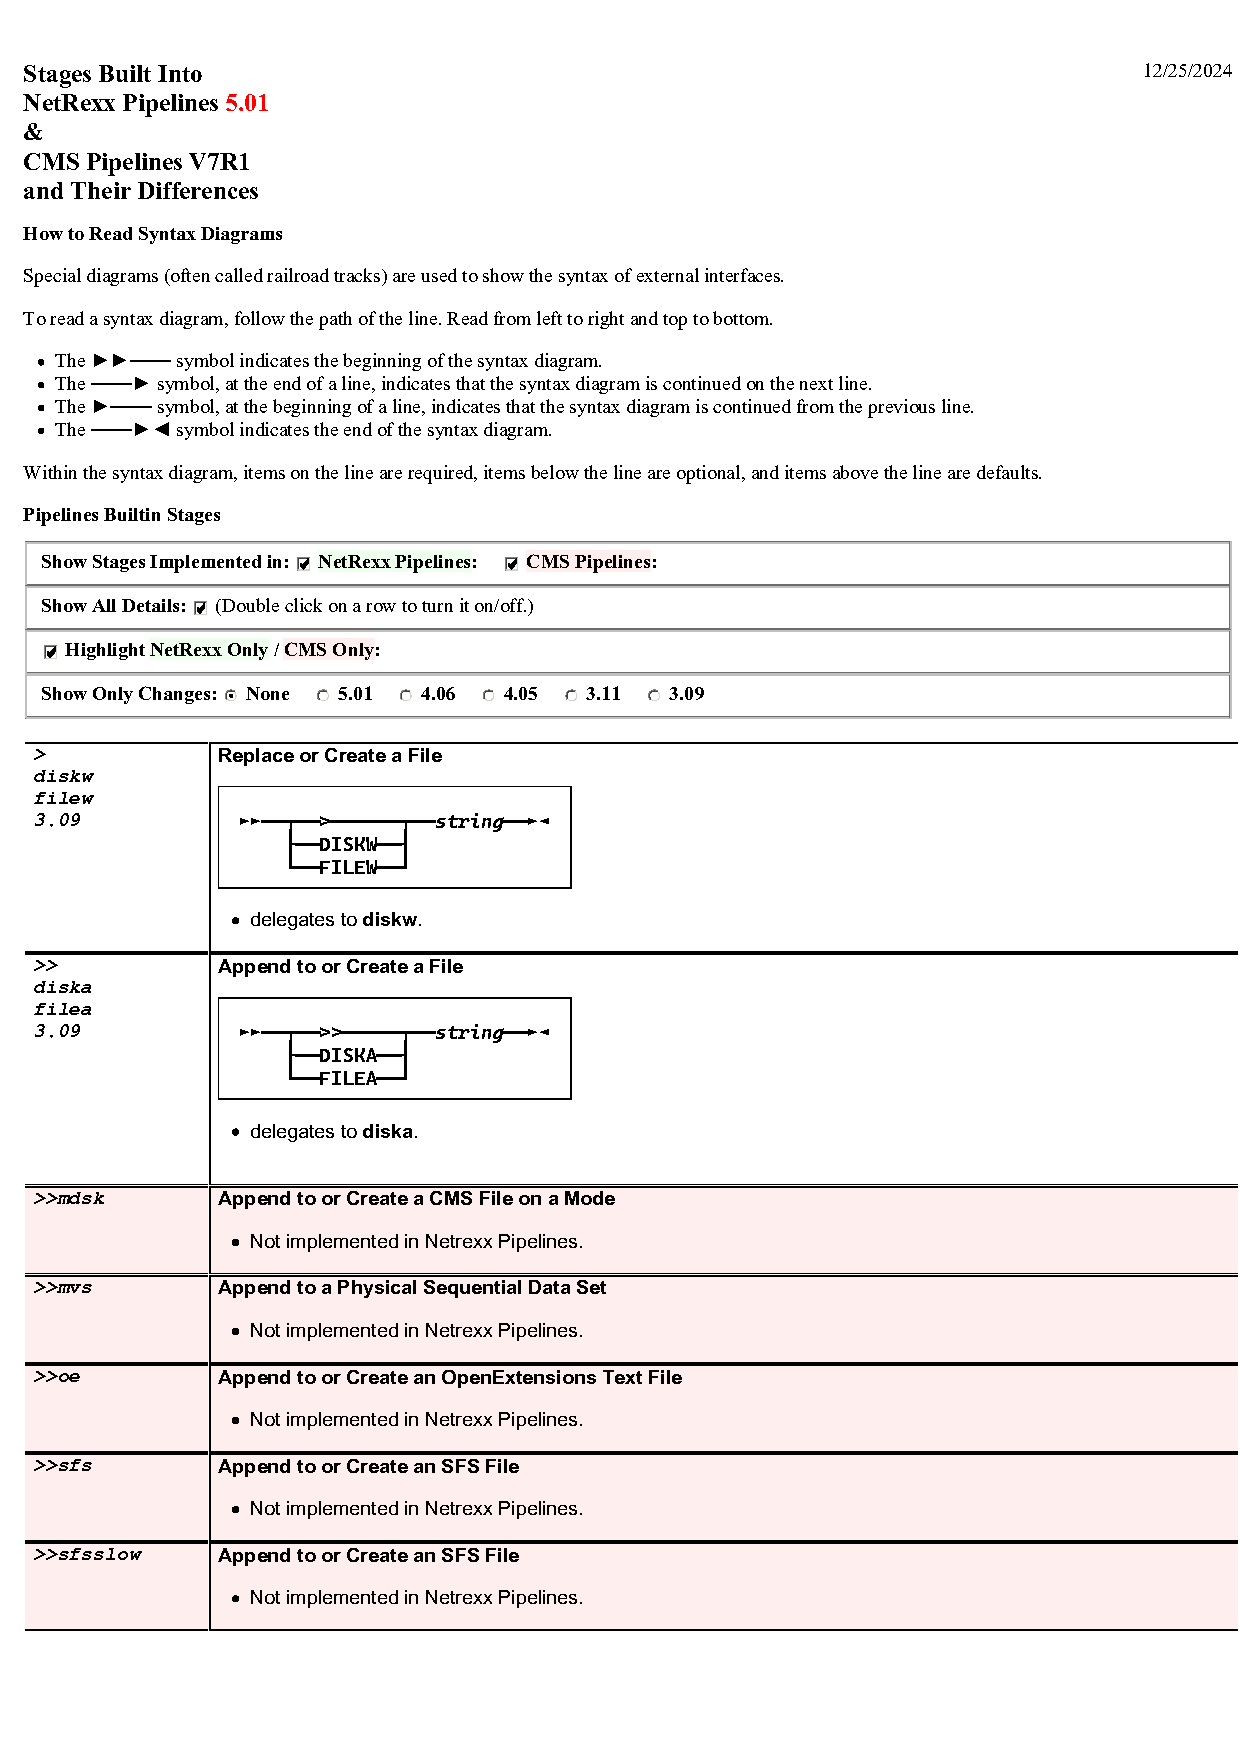
\includepdf[pages={1-13},nup=1x1,landscape=false]{stages.pdf}
\chapter{Appendix A}
\begin{verbatim}
.50  - Released May 30, 1999
         - Fixed a stall occurring when interrupted threads, with the interrupt
           caught by ThreadPool, were reused.
         - Fixed a thread safety problem in ELASTIC
         - Improved the timeout options in TCPDATA and TCPCLIENT, they also
           byte[] instead of strings.  This was done since converting to and
           from strings sometimes scrambles binary data (more research on
           encodings...)
         - Changed DELBLOCK it now handles byte[] to help keep tcpdata and
           tcpclient efficient.  The EOF option was broken, its fixed now.
         - Changed DISKR, DISKW and DISKA to handle byte[] when using streams.
         - Added INSERT which handles byte[].  This should be used instead of
           SPECS to add LF or CR .
         - Changes SERIALIZE to use byte[].
   0.49  - Released May 21, 1999
         - compiled with 1.2.1 and NetRexx 1.148
         - Added preliminary support added to .njp compiler for files containing
           java source!  See the (some what messy) java samples in vectort1.njp,
           overtest.njp and addtest4.njp
         - Added code to generate a dummy .nrx file containing the public class
           in a .java file.  This allows NetRexx to compile class that depend on
           the java source.
         - Modified sort to accept arguements in the same order as CMS
         - Fixed rc logic in drop stage
         - Fixed shortcut code for {n} where n is numeric.
   0.48  - Released May 16, 1999
         - Fixed a (nasty) bug involving reusing pipe objects.
         - Added the reuse() method to the stage class.  To use it override
           it in your stage.  It was added so there was a foolproof way to
           reset a stage when its pipe object is reused.  (doSetup is intended
           for use with dynamic arguements in call or added pipes)
         - Added the cont option and defaulted it to comma.
         - fixed return code logic in some stages and in selectInput/Output
         - Added the Emsg methods
         - Added arguement debug option (128)
         - There are no more final methods
         - Much improved error reporting from stages via new Emsg method
   0.47  - Released Jan 3, 1999
         - recompiled with 1.1.7A and netrexx 1.148
         - UNIQUE repaired?
         - Added stages to acess java objects easily
           VECTOR, VECTORR, VECTORW, VECTORA for java.util.vector
           ARRAY, ARRAYR, ARRAYW, ARRAYA for Object[]
           HASH, HASHR, HASHW, HASHA for java.util.Hashtable
           DICT, DICTR, DICTW, DICTA for java.util.Dictionary
           The hash stages mostly map directly to DICT stages.  The exception
           is HASHW which uses the clear() method of Hashtable.
         - Modified LITERAL to be able to put any object into a pipe
         - Modified pipe package to store arguements in a hashtable instead of
           a rexx stem - arguements can now be of any class.  Use the arg(null)
           method to get an object arguement.
   0.46a - Released Oct 14, 1998
         - recompiled with 1.1.7
         - TCPLISTEN now supports an input stream to be used to pace accepts
   0.46  - Released Sept 20, 1998
         - COMMAND, CHANGE, FILE, LOCATE, DROP, LOOKUP, TCPCLIENT, TCPLISTEN
           SQLSELECT, CONSOLE, TCPDATA, NOEOFBACK improved.
         - Jeff improved the testing process with the addition of the COMPARE
           stage, he also upgraded many of the tests.
         - Added the buildtests pipe, it builds a test script to be run with:
           test > output < console.data
         - Unexpected exceptions should no longer hang pipes
   0.45  - Released Sept 9, 1998
         * Recompile all your stages.  To fix a commit problem I had to
           change the _stage interface class...
         - tcpclient restart problems with oneresp active fixed.
         - commit now returns the current return code of the pipe.
         - fixed minor errors in tcpclient and diska.
   0.44  - Released Sept 8, 1998
         * a recompile of pipes using STEM is required
         - smart DISK, FILE and STEM stages now exist.
         - Made to and from synonoms for in and out in REXX and STRING stages.
         - Added stream option to DISKR and DISKW to read raw streams.
         - Added DISKSLOW and SERIALIZE stages.
         - Now DISK, DISKR, DISKW, DISKA and DISKSLOW have FILE synonyms.
         - Deadlock detection improvements.
         - TCPDATA & TCPCLIENT optimized once again.
         - selectAnyInput could deadlock - fixed.
         - interrupting a pipe now kills it - use this with care (ie. kill -9)
         - Pseudo methods njpRC() and njpObject() are reconized by the pipes
           compiler and return the pipe's RC or object respectivily.
   0.43  - Released August 30, 1998
         - Fixed deadlock dection to see commit deadlocks.
         - Added rest of code to handle improved StageError logic.
         - Added stage templates (template*.nrx) in the njpipes directory.
         - Added a debug flag (64) to trace all StageError rasied by the
           stage class.
   0.42  - Not released
         * A recompile of pipes using TCPCLIENT, TCPDATA is required.
         * A recompile of pipes using REXX, STRING, ZONE, CASEI is recommended.
         - Updated the comments in _stage to reflect the possible StageError
           and return codes that can be issued.
         - Added the DEBLOCK stage and reworked TCPDATA, TCPCLIENT & GATE.
         - Improved eofReport processing and added a new option 'either' that
           will trigger a StageError when any stream, input or output, severs.
         - Fixed variable subsitution so multiple variables passed to a stage
           will work.
         - Added the ability to pass thru arguements to callpipe and addpipe.
         - Fixed a problem with some StageExits requiring stage_reset methods.
         - Added a function to utils to help assign smarter name to classes
           generated by StageExits.
         - Added counter method to stage.  use to count external waits so
           deadlock/stall detection is not fooled.
   0.41  - Released August 23, 1998
         * removed OBJ2REXX, OBJ2STRING stages, use REXX and STRING stage
           modifiers.
         * pipes using TCPDATA, TCPCLIENT & LOOKUP should be recompiled
         - exhanced REXX stage modifier via an object2rexx improvement in
           pipes/utils.nrx
         - optimized ThreadPool startup times.  No setName and only use
           setPriority when its required.
         - made it possible to optimized stage startup time when arguements
           are static.  See TCPDATA, TCPCLIENT & LOOKUP
         - faq.txt enhanced
   0.40  - Released August 14, 1998
         * All pipes MUST be recompiled.  Old pipe class files will stall.
         - OBJ2REXX is depreciated and will be removed, use the REXX stage.
         - added REXX and STRING stages to convert objects entering and leaving
           a stage to rexx or string.  Inorder to avoid nasty class conflicts,
           REXX and STRING are implemented in _rexx and _string.  The compler
           adds the '_' when necessary (any stage can use this feature).
         - fixed an intermitant stall in callpipe (was completing too fast :-)
         - fixed a stall occuring between shortStreams and COMMAND
         - optimized pipe startup time in pipe.class and via the compiler.
         - optimized rc, commit, deadlock, threadpool code
   0.39  - Released August 9, 1998
         - WAIT_COMMIT and WAIT_ANY are now used in the call/addpipe logic
         - callpipe was not notifiing its pipe when ending leading to an
           very intermitant hang.
   0.38  - Released August 3, 1998
         * All your stages must be recompiled.  Recompile your pipes to
           exploit the pipe & thread pool performance improvements.
         - fixed and optimized commit logic.
         - implement a pool for pipes to decrease overhead.
         - implement a pool for threads to decrease overhead.
         - compiler fix to proprogate return codes from stageExits (thanks Jeff).
         - signal StageError('...  in all stageExits modified to
           signal StageError(13,'Error - 'pInfo' - ...
         - UNIQUE stage added by Jeff.  It exploits stageExit.
         - COMMAND stage was not starting its threads correctly.
         - SORTs in different pipes could corrupt each other.  Thanks René‚
   0.37  - Released July 25, 1998
         * A recompile of pipes using SORT is required
         - added NOEOFBACK, TOTARGET and FRTARGET.
         - removed a protected method from dump(), added arg() to the dump
         - upgraded SORT, sortRexx to exploit IRange and stageExit, optimized
           use, and factored the sort algorithm out of sort/sortRexx.
         - multiple sort stages no longer try to share static variables...
         - the compiler just uses the stage name (not args) when naming stages
   0.36  - Released July 19, 1998
         * A recompile of ALL pipes with stages using IRANGE is required.
           (CHANGE, DEAL, JOINCONT, LOCATE, LOOKUP, PICK, XLATE & ZONE)
         * pipes using NFIND, NLOCATE, STRNFIND or SORT also need to be
           recompiled
         - Added BuildIRangeExit and other methods to an updated IRange
           class.  Using 'zone range stage ...' will be faster than
           'stage range ...' when the range consists of n.c or n-c (s).
         - NFIND, NLOCATE, STRNFIND implemented via stageExit and NOT
         - Fixed bugs in, JUXTAPOSE, FIND, STRFIND, SORT, COMMAND, CHANGE
         - The compiler was not calling stageExit in the correct order when
           several calls were needed to build the stage.  (zone w1 nfind..)
   0.35  - Released July 16, 1998
         - Jeff Hennick pointed out a bugglet that effected LOOKUP, ZONE and
           PICK that could occur with complex ranges, I found another bug in
           strliteral
         - Jeff Hennick updated this doc with information on IRange and DString
   0.35  - Released July 15, 1998
         * A recompile of ALL pipes using ZONE, TCPCLIENT, TCPDATA, PREFIX
           and APPEND is required.
         - prefix and append can now be labeled, tcpclient and tcpdata
           now use a stage, instead of a pipe, to group data.
         - added compiler support for negitive stream numbers.  This is
           intended to be used by stageExit.  See append, prefix, tcpdata
           and tcpclient.
         - Redefined rexxArg() and stageArg() to simplify the compiler.
         - selection stages are no longer defined as final.
         - SelectInput(0) and selectOutput(0) are always called by the
           stage implementation so they can be overridden...
         - Reimplemented ZONE using stageExit, added CASEI using the same
           technique.  In theory NOT could be done the same way but, to
           avoid some recursion problems NOT is staying in the compiler.
         - StageExit modified to allow it to pass back another stage to
           call.  see ZONE, CASEI and NOT.
   0.34  - Released July 11, 1998
         - minor reportEOF(any) logic fix
         - improved command stage, threads used to process stdout and stderr.
           added zone, pad, lookup, pick, upgraded juxtapose, fixed bugs in
           specs & buffer.
         - added pad option to setIRange method
   0.33  - Released July 5, 1998
         - added rexxArg() and stageArg() methods to utils.nrx for use by the
$          compiler to query stages about what they expect their arguments to
           contain.  This allowed the compiler to be simplified.
$        - locate now handles null arguments correctly.  literals now include
           leading blanks.  Thanks for pointing out the problem René.
         - René Jansen contributed the timestamp stage.
         - logic modified to stop output() from getting an EOF when the output
           object has been peeked.  The peek status is also displayed by the
           dump() method and hense by deadlocks.
         - minor specs bug fixes (next.n and nextw.n output specs now work)
         - modified the compiler to invoke stageExit(rexx,rexx) method.  This
           allows stages to generate code and/or change the pipe topology.  See
           specs, append, prefix, change and xnop, in the stages directory.
         - modified StageError in preparation for usage changes.
         - removed the Range class - Jeff's code is better and anything that
           could be done with Range can be done using stageExit.
         - Jeff fixed bugs in change and join and added:
           fblock          joincont        notinside       outside
           inside
   0.32  - Released June 20, 1998
           Jeff updated these stages adding a few new ones too:
           abbrev          between         split           locate
           nlocate         strnfind        strfind         nfind
           find            chop
         - minor docuementation updates
         - the Range class is depreciated and will be removed.  Use the
           replacements Jeff created (see pipes\utils.nrx and stages\).
   0.31  - Released June 17, 1998
         - modified count, drop, take and deal to handle non rexx objects
           when possible
   0.31  - Released June 16, 1998
         - improved eofReport(ANY) logic to trigger when waiting on output
           and a different output stream severs.
         - factored the source for utils.class out of stages so there is
           a class to add (probably static) shared methods for all stages
         - fixed a deadlock that occured between shortStreams and exit
           (severInput)
         - Jeff Hennick updated many stages to work at CMS or near CMS levels.
           append          deal            join            strfrlabel      xlate
           buffer          drop            literal         strliteral
           change          fanin           locate          strtolabel
           console         fanout          split           take
           count           frlabel         strfind         tokenize
           All of Jeff's changes are GNUed.  See CopyLeft.txt in the njpipes
           directory.
   0.30  - Released May 24, 1998
         - fixed logic in core classes to post all pending severs and not
           clear them too early either, this corrects a problem seen on
           Multiprocessor machines.
   0.29  - www page update (docuemention) May 20
         - deadlock section updated
         - installation verification example corrected!
   0.29  - Released May 17, 1998
         - added obj2rexx stage, tolabel stage courtesy of Chuck Moore.
         - enhanced change to support a single range
         - Added setJITCache(Hashtable) method to pipes.  This can be used
           to build a global object cache in programs calling pipes.  The name
           of the Hasttable is passed to pipe/callpipe/addpipe via a cache
           parameter.
         - Added support for reportEof options.  This support is not too
           well tested - some good testcases are needed.
   0.28  - Released May 9, 1998
         - Enhanced parsing in specs (word2.1 would work, word 2.1 would not)
         - Fixed COPY for a NT jit bug, fixed locate so NOT LOCATE would
           work, updated LITERAL not to use more than one exit(rc)
         - Fixed a compiler problem that would hit multistreamed pipes using
           append or prefix.
         - Any options not consumed by njp are passed on to nrc
           and java.  Mainly for use from the command line, use with care
           in .njp files...
         - Fixed shortStreams() so it works correctly when shorting streams
           in a stage with multiple streams.
         - Tested all 8 addpipe forms and fixed runtime to work with all
           test cases
         - modified filternjp to accept *in and *out without additional labels
         - reenabled stop() in exit code...
         - added gate, dam, tokenize, juxtapose and courtesy of Chuck Moore,
           frlabel stages
   0.27  - Released May 3, 1998
         - Automated the generation of in/outStream calls.  For this to work
           the labels need to be of the form *in0: or *out0: where the '0' is
           replaced by the input or output stream to connect to.
         - Fixed compiler/filter problems with stema
         - Tighted range checking code in specs, fixed problem with delimited
           ranges.  Specs was compiling the NetRexx EXIT command...
         - Fixed a problem where output was not see that objects were
           consumed when using sipping pipes...
         - Fixed a problem where severing an output stream did not cause the
           stages stacked on the node's outlist to see the sever
         - Fixed a problem where the stage issuing a callpipe was not seeing
           the called pipe end
         - Added debug option to pipes compiler
         - Repaired commit and added commit levels to dump() method
         - Fixed problems with callpipe servering several outputs, unstacking
           the saved stream was selecting it...
         - Modified tcpclient and tcpdata to use a secondary thread to
           recieve the tcpip inputs.
         - Now keep a referenced object for each pipe/stage so the JIT does
           not throw away its work and call/addpipes in loops work faster.
         - in/outStreamState now return -1 when autocommit is enabled and
           the stream is unused.
   0.26  - Released April 26, 1998
   - Added selection methods to compiler (see getRange in section 4 and
           the locate stage an example#
         - Added the specs stage.  The compiler builds a stage to process the
           specs, reducing overhead.
         - Added tcp/ip stages
         - Fixed problems with severs using addpipe
   0.25  - Optimized some stages using jinsight from www.alphaworks.ibm.com.
           This more than doubled the speed of some stages.
         - fixed bugs in fanin, diskw
         - Added netrexx filters to extract pipes, extended the functions
           of .njp files (multiple pipes in a file and .njp files can now
           contain netrexx code with pipe/callpipe/addpipe)
         - fixed a timing bug in deadlock detection.
         - xlate and sqlselect stages contributed by René Jansen added
   0.24  - Release Feb 98
         - modified the compiler so the syntax of pipes from the command line
           is the same as pipes from .njp files
         - added the sort stage, the sortClass interface and the sortRexx
           example implementation
         - added the timer stage
   0.23  - fixed minor compiler errors (20 Dec 97)
         - not stage modifier added.
         - errors in this page corrected, NT install information added.
         - modified diskr/diskw to use Buffered Streams.
   0.22  - second public release
   0.21  - enabled auto commit, stages start at a commit level of -2 and
           commit to a level of -1 at the first readto, peekto or output.
           nocommit disables the auto commit.  This feature has not been
           completely tested (yet).
         - fixed compiler not to call netrexx if one of its pipes deadlocks
   0.20  - Upgraded to May version of the NetRexx compiler (Thanks Mike!)
           this changed the compiler interface.  NetRexx from May 10 or
           later is now required.
         - nocommit added to _stages, though its a nop for now
         - modified the compiler class to use the May 10th NetRexx compiler
   0.19  - initial public release (4 May 97)
\end{verbatim}
\backmatter
\listoffigures
\listoftables
\lstlistoflistings
\printindex
\clearpage
\psset{unit=1in}


\chapter{Differences with CMS Pipelines}
The goal of this implementation is to be as close as possible to the
the CMS version of Pipelines. A few differences are unavoidable.

\begin{itemize}
\item The character set is Unicode and not EBCDIC, as Unicode is the
  character set of the underlying Java platform
\item As shells are different, many 3270 related stages are not
  implemented
 \item Pipes need to be quoted on the Windows and Unix command lines;
   the Workspace for \nr{} (\emph{nrws}) environment is an exception to this rule
\item The mainframe is record-oriented in many stages, Pipelines for \nr{} does
  an approximation of this
\item Pipelines on the mainframe is an interpreted language with
  components as the scanner and the dispatcher; the \nr{}
  version is compiled to Java .class files by \emph{pipc}, the pipes
  compiler, and dispatched as threads by the JVM.
\item The mainframe pipes dispatcher is not multiprocessor enabled. In
  Pipelines for \nr{} all tasks (stages) are dispatched over all available
  processors in parallel.
  \item The fact that pipes run from \nr{} implies that they can be
    used in Java source. In previous releases there was more direct
    support for this; this has lapsed due to changes in the way a java
    toolchain works. This support can be restored in future releases.
  \item To put the content of  a \nr{} variable in a pipe
    specification in a \nr{} program, there is a \texttt{\{\}}
    mechanism. In CMS the pipe would be quoted in the Rexx source and you would unquote sections to get a similiar effect.
\end{itemize}

\begin{pspicture}(3.5,1in)
  \psbarcode{\isbn}{includetext guardwhitespace}{isbn}
\end{pspicture}
\end{document} 
